\documentclass[12pt]{article}

\usepackage[]{graphicx}
\usepackage[]{color}
\usepackage{alltt}
\usepackage{subcaption}
\usepackage{float}   % in the preamble


%for longtable
\usepackage{longtable}


\newcommand{\mytitle}{Uncovering Structural Relations in the ifo Business
Survey}
\newcommand{\myname}{Jakob Freytag, Daniel Gloukhman, Dominik Pitz}


\usepackage[a4paper, width = 160mm, top = 35mm, bottom = 30mm, 
bindingoffset = 0mm]{geometry}
\usepackage[utf8]{inputenc}
\usepackage{ragged2e}
\usepackage{xcolor}
\usepackage{amsthm}
\theoremstyle{plain}

\theoremstyle{definition}
\newtheorem{defn}{Definition}[section]
\usepackage[round, comma]{natbib}
\usepackage{fancyhdr}
\newcommand{\changefont}{%
    \fontsize{8}{11}\selectfont
}
       % For professional-looking tables
     % To allow tables to span multiple pages

\usepackage{hyperref}
\usepackage{amsmath}
\usepackage{amsfonts}
\usepackage{amssymb}
\usepackage{algorithm}
\usepackage{algpseudocode}
\usepackage{array}
\usepackage{booktabs}
\usepackage{caption}
\usepackage{subcaption}
\usepackage{tabularx}
\hypersetup{
  colorlinks = true,
  linkcolor = black,
  urlcolor = black,
  citecolor = black}
\pagestyle{fancy}
\fancyhead{}
\fancyhead[R]{\changefont{\mytitle}}
\fancyfoot{}
\fancyfoot[R]{\thepage}
\setlength{\headheight}{14.5pt}
\setlength{\parindent}{0pt}
\interfootnotelinepenalty = 10000


\begin{document}


% FRONT PAGE -------------------------------------------------------------------
 
\begin{titlepage}
\begin{center}
    
\LARGE
Consulting Project Report

\vspace{0.5cm}
      
\rule{\textwidth}{1.5pt}
\LARGE
\textbf{\mytitle}
\rule{\textwidth}{1.5pt}
   
\vspace{0.5cm}
      
\large
Department of Statistics \\
Ludwig-Maximilians-Universität München 

\vfill

\Large
\textbf{\myname}

\vfill

\large
Munich, August 22\textsuperscript{th}, 2025
      
\vfill


\includegraphics[width = 0.4\textwidth]{sigillum.png}

\vfill

\normalsize

Project Parter: Dr. Klaus Wohlrabe, ifo Institute \\
Supervised by Dr. Fabian Scheipl, LMU 

\end{center}
\end{titlepage}



\pagenumbering{Roman}
\newpage

\begin{abstract}
The ifo Business Survey is a monthly poll conducted by the ifo Institute
for Economic Research in Germany, gathering responses to self-assessment questions on topics such as business
expectation or current situation from multiple companies 
across different sectors. Its most popular indicator is the ifo Business Climate Index, aggregating the business sentiment across all industries.
While the index is well-established as a leading indicator, the full potential of
the time series of the underlying sub-aggregates remains largely unexplored.
This report accompanies the consulting project, in which we aimed to uncover potential relationships by taking a closer look
at the manufacturing industry, whose business climate is closely linked to the
main index. By analyzing the industry’s sub-aggregates over time, we examine how their interactions with the manufacturing business climate evolve
and whether certain sub-aggregates can serve as early indicators of turning
points. Detecting such patterns could enhance the economic assessments accompanying the monthly release of the ifo Business Climate Index. \\
We begin with a comprehensive correlation analysis to map the relationships between individual industries and the main manufacturing index. These relationships are further examined by a Granger causality analysis, where we find that when formally tested, almost all individual subseries are Granger causal, but their information gain is negligible. We then use different approaches to identify subsets which seem to be especially indicative, such as an elastic net, a scoring model and clustering based on their cross-correlation function with the main index. At last, we asses, whether we can predict economic turning points of the main index, using Markov Switching models applied to the sub-aggregates. In this setting, neither individual, nor grouped series were able to meaningfully indicate the main turning points.  
\end{abstract}


\newpage
\tableofcontents

%%%% if you would want to include material overview
%%%% use one of the following in addition
\newpage
\listoffigures
\newpage
\listoftables
\newpage


% CHAPTERS ---------------------------------------------------------------------
\pagenumbering{arabic}
    


%--------------------------------------------------------------------------------
\section{Introduction}
\label{ch:intro}
The ifo Business Survey is a monthly poll conducted since 1949 by the ifo Institute
for Economic Research in Germany, gathering responses from multiple firms
across different sectors \citep{sauer2023handbook}. It includes self-assessment questions on topics such as the current business situation or expectation and also more specific questions, such as production plans. The answers are aggregated hierarchically, ranging from small specific industries up to four main sectors: manufacturing industry, construction industry, service sector and trade. The survey's most popular indicator is the ifo Business Climate Index, consisting of the the two questions on current business situation and expectation, aggregated across all industries. The index is well-established as a leading indicator, with many studies examining its predictive power for economic variables such as the national GDP. However, the underlying structures within the business survey are largely unexplored so far. In this project, we will take a closer look on the many time series underlying the ifo Business Climate Index. Rather than focusing on building a rigorously validated predictive model, this project seeks to uncover potential relationships in these time series through a descriptive analysis of historical data.


\begin{figure}[H]
    \centering
    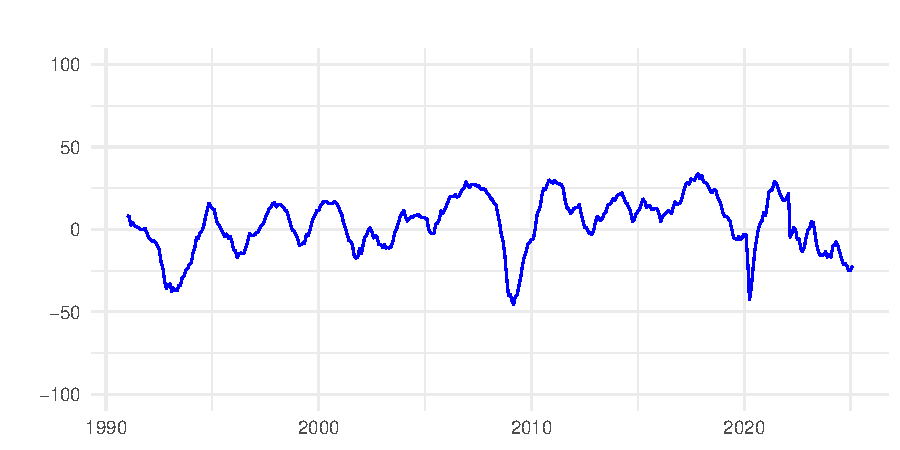
\includegraphics[width=0.5\linewidth]{JakobPlots/main_index_plot.pdf}
    \caption{ifo Business Climate Index over the period considered in this analysis.}
    \label{fig:main_index}
\end{figure}

\subsubsection{Data}
Within the survey, we focus on the manufacturing sector, one of the main drivers of the German economy \citep{sauer2023handbook}. In our dataset, the highest aggregation level corresponds to the entire manufacturing sector as a whole. One level below this aggregate in the hierarchical structure, there are 21 constituent industries such as the automotive industry or the machinery and equipment industry. We refer to these as level~1 aggregates. In total, five levels exist, though our analysis mainly considers level~1 and level~2 aggregates. Industry aggregates are identified by an industry code based on the official classification of economic activities of the German Federal Statistical Office \citep{sauer2023handbook}. For example, the main aggregate is coded \texttt{C0000000}, with the letter \texttt{C} denoting the manufacturing industry and the digits indicating the aggregation level, which is the the highest level in this case, as all digits are zero. Industries at level~1 are identified by the first two digits, e.g.\ \texttt{C2800000} for machinery and equipment. Each additional nonzero digit specifies one further level, so \texttt{C2810000} corresponds to a level~2 sub-aggregate of machinery. In our study we define level~1 aggregates (codes \texttt{C} followed by two digits) as sectors. Table~\ref{tab:sectors} provides an overview of the manufacturing sectors covered by the survey. The abbreviations for all other industry codes can be found in the appendix~\ref{ch:appendix}.

\begin{table}[H]
    \centering
    \small
    \begin{tabularx}{\textwidth}{lX}
        \toprule
        \textbf{Code} & \textbf{Sector} \\
        \midrule
        C1000000 & Manufacture of food products \\
        C1100000 & Manufacture of beverages \\
        C1300000 & Manufacture of textiles \\
        C1400000 & Manufacture of wearing apparel \\
        C1500000 & Manufacture of leather and related products \\
        C1600000 & Manufacture of wood and of products of wood and cork, except furniture; manufacture of articles of straw and plaiting materials \\
        C1700000 & Manufacture of paper and paper products \\
        C1800000 & Printing and reproduction of recorded media \\
        C1900000 & Manufacture of coke and refined petroleum products \\
        C2000000 & Manufacture of chemicals and chemical products \\
        C2100000 & Manufacture of basic pharmaceutical products and pharmaceutical preparations \\
        C2200000 & Manufacture of rubber and plastic products \\
        C2300000 & Manufacture of other non-metallic mineral products \\
        C2400000 & Manufacture of basic metals \\
        C2500000 & Manufacture of fabricated metal products, except machinery and equipment \\
        C2600000 & Manufacture of computer, electronic and optical products \\
        C2700000 & Manufacture of electrical equipment \\
        C2800000 & Manufacture of machinery and equipment n.e.c. \\
        C2900000 & Manufacture of motor vehicles, trailers and semi-trailers \\
        C3000000 & Manufacture of other transport equipment \\
        \bottomrule
    \end{tabularx}
    \caption{Overview of manufacturing sectors covered by the ifo Business Survey}
    \label{tab:sectors}
\end{table}

The ifo survey covers multiple questions on the current situation and expectations. For consistency, we restrict our analysis to questions and aggregates that have been included continuously from 1991 up to February 2025, the last month in our dataset. Furthermore, we only include questions that are asked on a monthly basis to avoid mixing indices of different frequencies (monthly, quarterly, or yearly). Aggregates with any missing values for a given question during this period were excluded. Table~\ref{tab:ifo_terms} lists the survey questions and their corresponding abbreviations.

\begin{table}[H]
\small
\centering
\label{tab:ifo_terms}
\begin{tabularx}{\textwidth}{|r|l|X|}
\toprule
\textbf{Abbreviation} & \textbf{German Term} & \textbf{English Translation} \\
\midrule
KLD & Geschäftsklima & Business Climate \\
GUS & Geschäftslage Beurteilung & Business Situation Assessment \\
GES & Geschäftslage Erwartungen & Business Situation Expectations \\
LUS & Fertigwarenlager Beurteilung & Finished Goods Inventory Assessment \\
BUS & Auftragsbestand Beurteilung & Order Backlog Assessment \\
XUS & Auftragsbestand Beurteilung Export & Export Order Backlog Assessment \\
AVS & Nachfrage gegen Vormonat & Demand compared to Previous Month \\
BVS & Auftragsbestand gegen Vormonat & Order Backlog compared to Previous Month \\
QVS & Produktion gegen Vormonat & Production compared to Previous Month \\
PVS & Preise gegen Vormonat & Prices compared to Previous Month \\
QES & Produktionspläne & Production Plans \\
PWS & Preiserwartungen & Price Expectations \\
XES & Exporterwartungen & Export Expectations \\
BES & Beschäftigtenerwartungen & Employment Expectations \\
PRS & Produktivitätserwartungen & Productivity Expectations \\
\bottomrule
\end{tabularx}
\caption{ifo Business Survey questions and their translations.}
\label{tab:ifo_terms}
\end{table}

In our analysis we define the level~0 aggregate of the business climate question (KLD) for the manufacturing sector as the main index, which serves as the central reference point throughout the study.


\newpage
%--------------------------------------------------------------------------------

%--------------------------------------------------------------------------------
\section{Correlation Analysis}
\label{ch:corr}
\subsection{Analysis Setup}

\subsubsection{Correlation Analysis Approach}
The central aim of the correlation analysis is to better understand how individual industries relate to the overall dynamics of the manufacturing sector. In particular, we address two guiding research questions. First, we ask whether there is a systematic \textit{lead/lag structure} between industry-level indicators and the main manufacturing index. Identifying such structures would reveal which industries tend to anticipate movements in the aggregate climate and which instead follow with a delay. Second, we investigate whether it is possible to identify \textit{stable subsets of industries} that, across different survey questions and time windows, consistently capture the evolution of the main index. The existence of such subsets would suggest that certain industries carry disproportionate informational value for monitoring the business cycle.

To answer these questions, we adopt a multi-step approach. We begin with a set of \textit{full-sample and rolling window analyses} to estimate correlations between industry-specific indicators and the main index over time. This allows us to detect both long-term structural relationships and short-term temporal fluctuations. Next, we apply a \textit{ranking-based consensus analysis}, which tracks how the relative importance of industries changes across questions and windows. This step provides a way to monitor stability and detect re-orderings in the correlation structure. Finally, we develop a \textit{scoring model} that integrates information across time and questions in order to identify those industries that remain consistently close to the main index. Taken together, these steps provide a framework for moving beyond one-off correlation estimates towards a systematic evaluation of persistence, stability, and cross-question robustness.

The focus throughout is on correlations between the survey’s main manufacturing index and the industry-level indicators. All industry codes are analyzed individually, and we highlight industries whose correlations are either particularly strong or reveal distinctive lead/lag patterns. These industries are of special interest as they may function as early-warning signals or as anchors for constructing composite indicators.

\subsubsection{Data Structure}
The structure of the underlying data introduces important considerations for the correlation analysis. Industry codes are distributed unequally across sectors and hierarchical levels, as illustrated in Figure~\ref{fig:industries_by_sector}. This imbalance has non-trivial effects: rather than distorting results, the over-representation of certain sectors appears to \textit{reinforce} the observed correlation structure. In particular, retaining the natural weighting implied by the hierarchy yields stronger and more coherent correlations between industry-level indicators and the main question than alternative approaches where correlations are first aggregated within sectors (e.g., by mean or median) and then averaged across sector values. 

\begin{figure}[H]
    \centering
    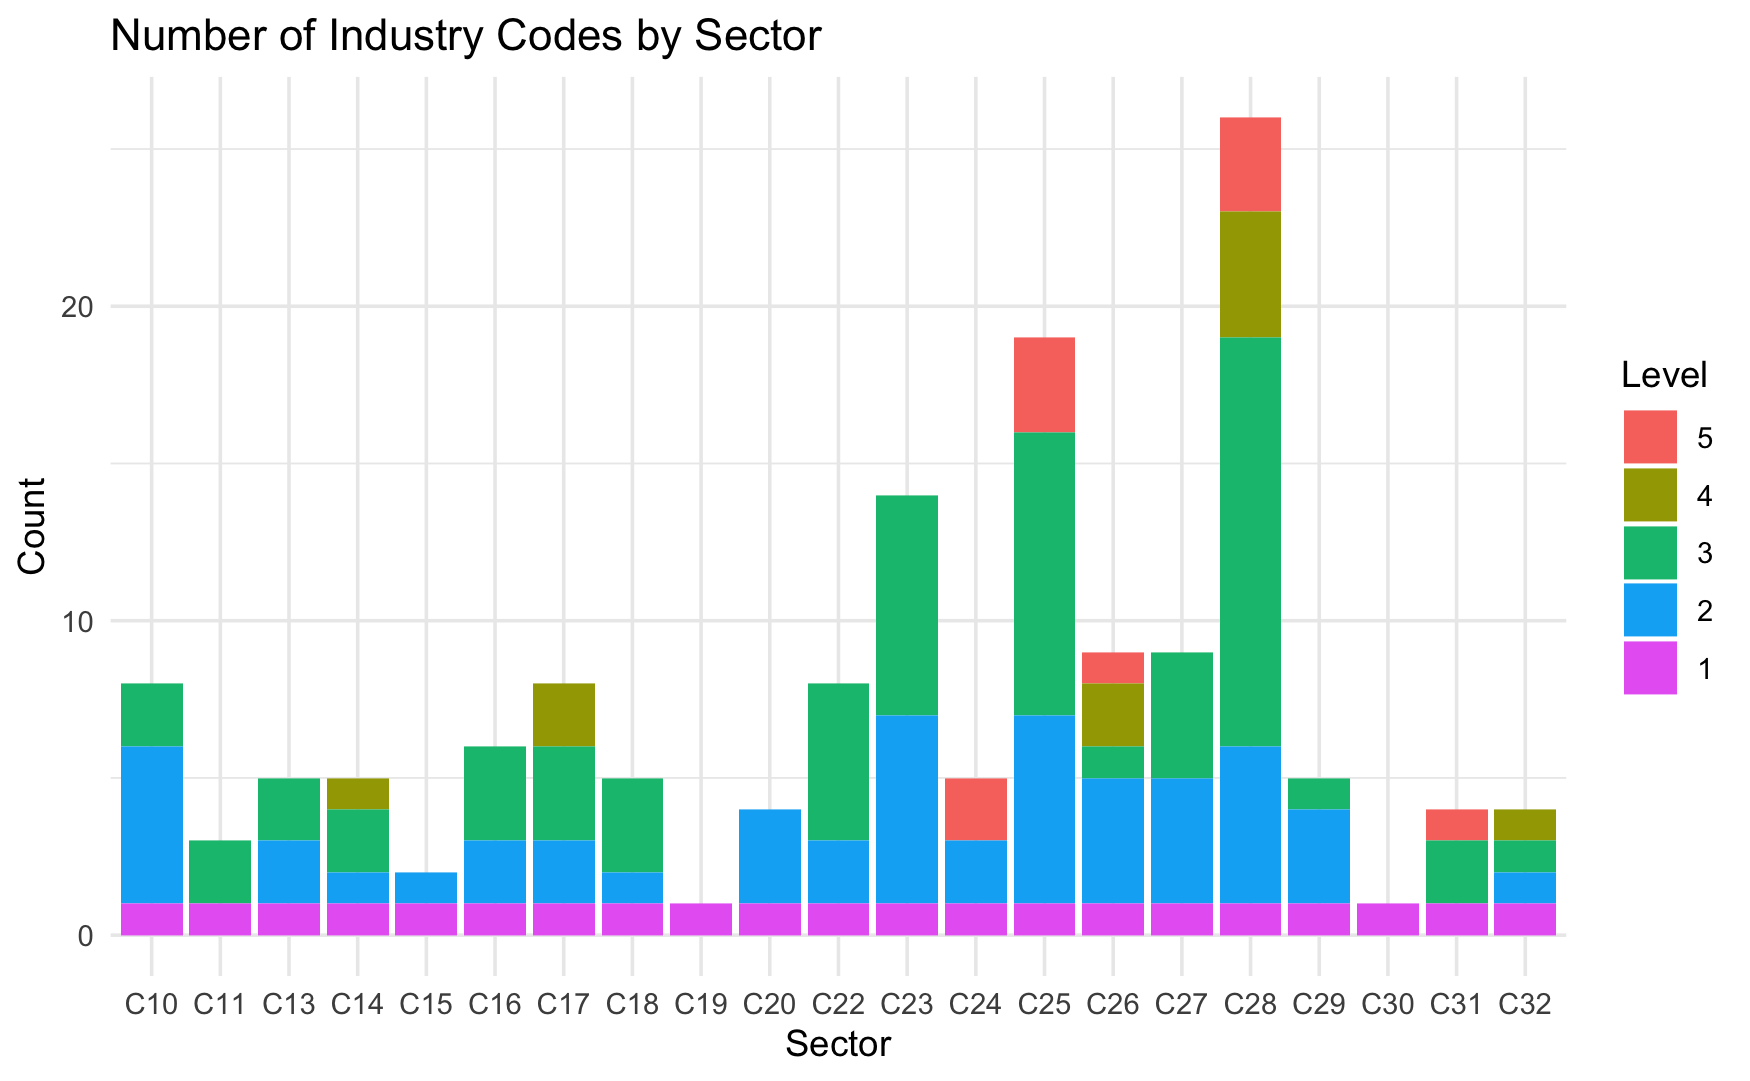
\includegraphics[width=0.7\linewidth]{DominikPlots/as_industries_by_sector.png}
    \caption{Number of industry codes by sector and hierarchical level.}
    \label{fig:industries_by_sector}
\end{figure}

This observation suggests that the hierarchical design of the industry codes reflects genuine structural dependencies in the data. For this reason, levels 4--5 of the hierarchy, which contain relatively sparse numbers of codes, are analyzed separately to avoid dilution effects. An overview of the manufacturing sectors included in the survey is provided in Table~\ref{tab:sectors}, while Figure~\ref{fig:industries_by_sector} summarizes the distribution of industry codes across sectors and levels.



\subsubsection{Stationarity}
\label{stationarity}
Stationarity of indices is often regarded as a prerequisite for correlation analysis, since the presence of common trends can artificially inflate correlations by introducing dependence driven by trend alone.  

In our dataset, however, not all industry codes are stationary. As illustrated in Figure~\ref{fig:comparison_earlypred_profiles}, many industry codes show a stationary KLD index over time. Yet if we required full stationarity across all questions and time windows, no industry code would satisfy this condition.  

\begin{figure}[H]
    \centering
    \begin{subfigure}[t]{0.48\linewidth}
        \centering
        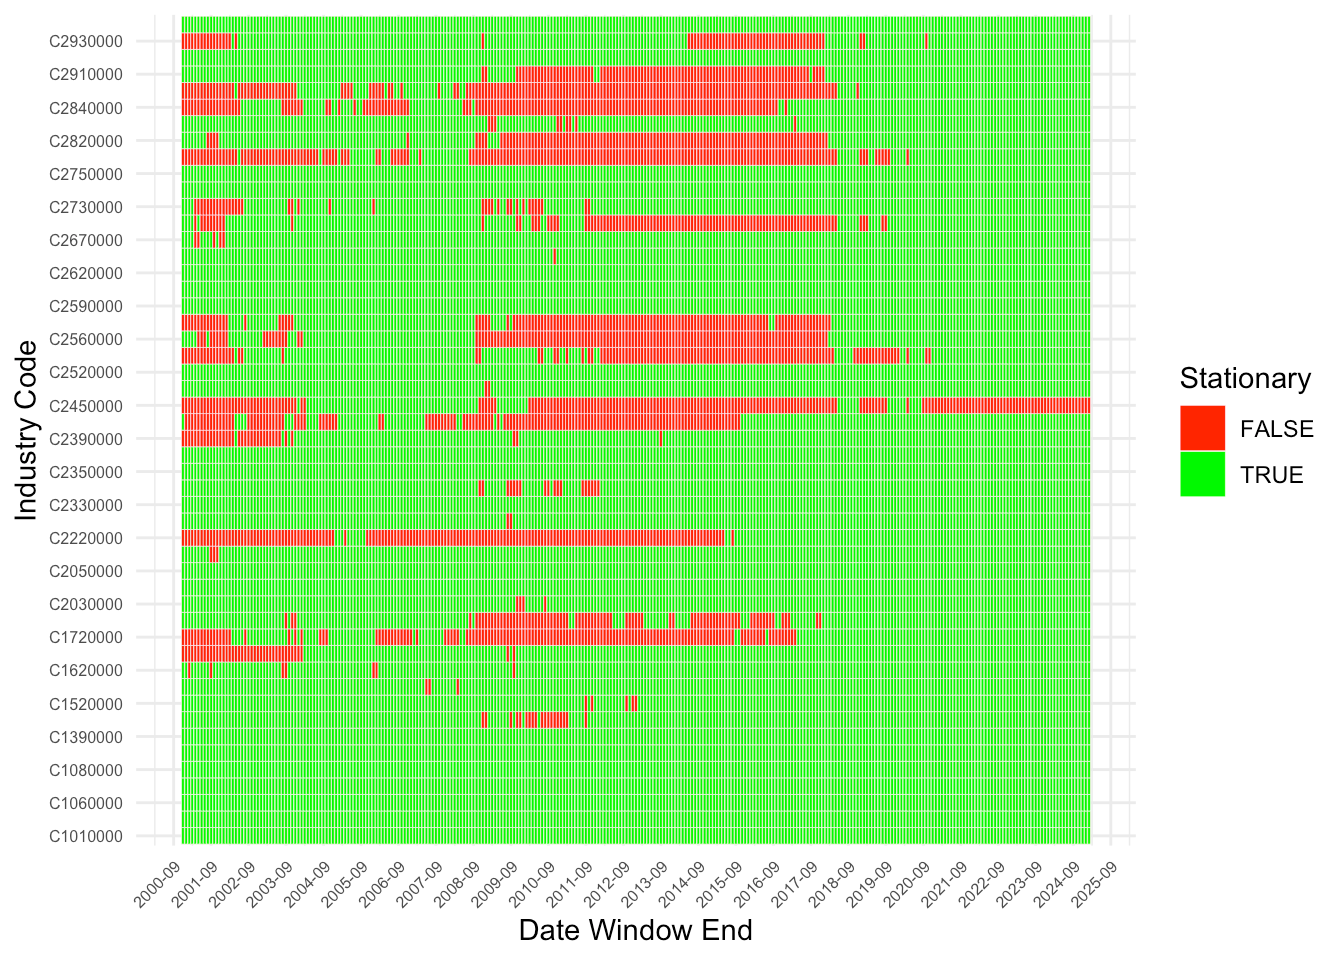
\includegraphics[width=\linewidth]{DominikPlots/as_stat_kld.png}
        \caption{Stationary industries (KLD).}
        \label{fig:stat_kld}
    \end{subfigure}%
    \hfill
    \begin{subfigure}[t]{0.48\linewidth}
        \centering
        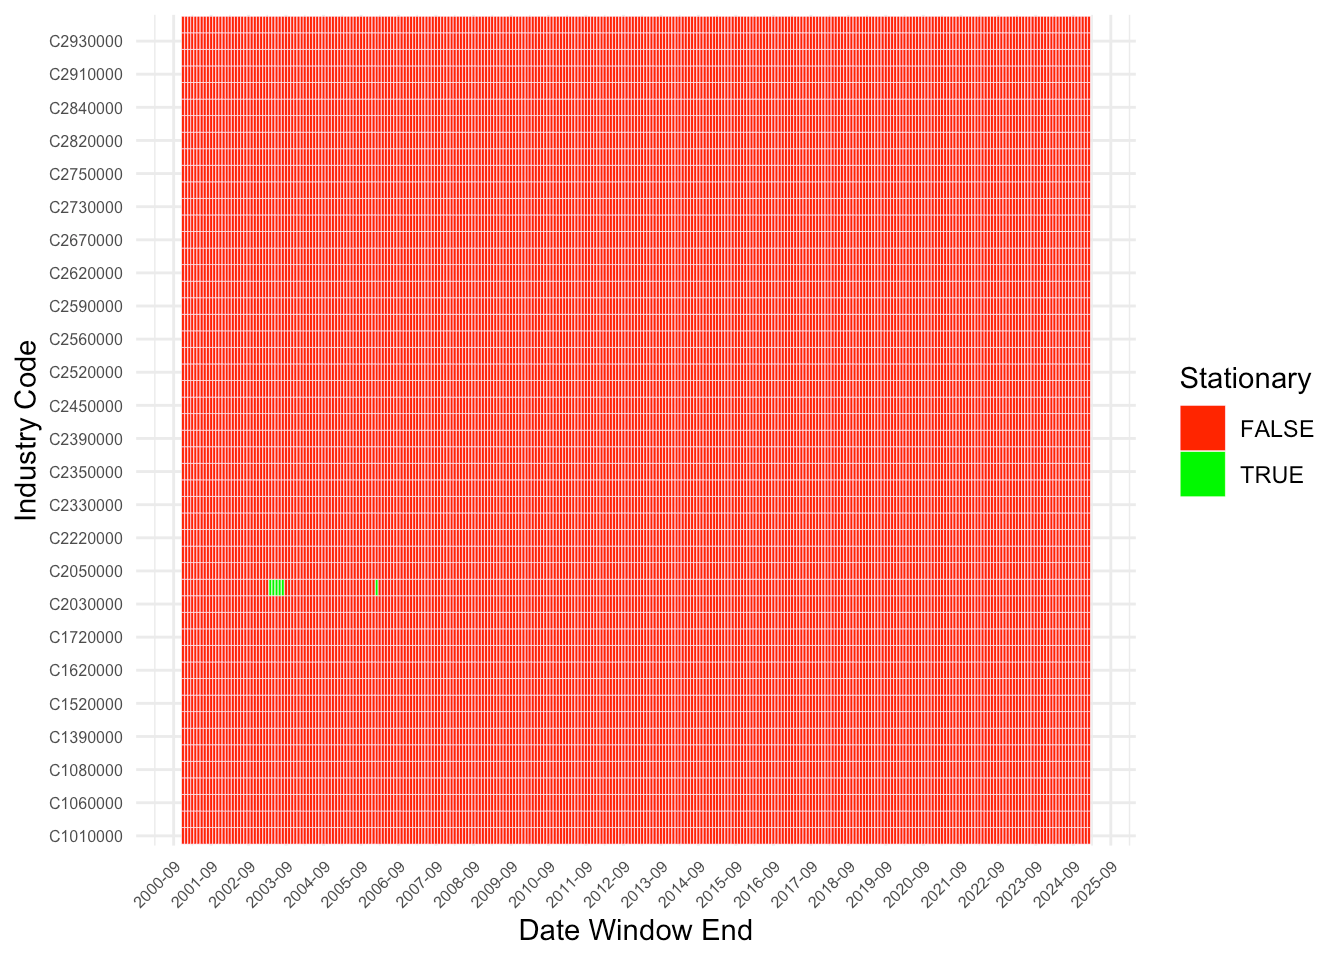
\includegraphics[width=\linewidth]{DominikPlots/as_stat_overall.png}
        \caption{Stationary industries (all questions).}
        \label{fig:stat_overall}
    \end{subfigure}
    \caption{Comparison of stationarity across time windows and questions.}
    \label{fig:comparison_earlypred_profiles}
\end{figure}

For the purposes of this study, we therefore did not impose stationarity as a strict requirement. While stationarity is generally desirable, excluding non-stationary series would eliminate too much information. Allowing for non-stationary indices may lead to higher measured correlations compared to the strict statistical definition, but in an economic context this is not necessarily problematic. In fact, when trends dominate certain rolling windows, correlations in trend may represent economically meaningful co-movement. From this perspective, we do not distinguish between ``true'' correlation and correlation driven by shared trends, as both can provide valuable insights into cyclical dynamics.  



\subsubsection{Correlation Metrics}
To quantify the relationship between industry-level indicators and the main manufacturing index, we employ two complementary measures: \textit{cross-correlation} and \textit{distance correlation}. Using both metrics allows us to balance interpretability with sensitivity to nonlinear dependencies.

\vspace{\baselineskip}
\textbf{Cross-correlation:}  
Cross-correlation, implemented via \texttt{stats::ccf}, measures the linear association between two time series at different leads and lags. It provides both the direction and magnitude of potential lead--lag structures. Because of its direct interpretability in terms of timing and sign, cross-correlation serves as the primary tool for detecting industries that anticipate or follow the dynamics of the main index.

\vspace{\baselineskip}
\textbf{Distance correlation:}  
Distance correlation, implemented via \texttt{energy::dcor}, extends beyond linear relationships by detecting any form of statistical dependence, including nonlinear or nonmonotonic structures. A key property of distance correlation is that it equals zero if and only if the variables are independent. In our setting, it thus provides an upper bound relative to linear correlation ($|\rho|$) and signals whether cross-correlation may understate the strength of dependencies. The measure was introduced and studied in detail by \citet{Szekely2007}.

\vspace{\baselineskip}
\vspace{\baselineskip}
Cross-correlation provides an intuitive baseline for interpreting the temporal structure of dependencies. Distance correlation, in turn, validates these findings by checking whether the relationships are predominantly linear or whether nonlinearities play a substantial role. In practice, both metrics yield strikingly similar structures (Figures~\ref{fig:median_ccf} and \ref{fig:median_dcor}), suggesting that linear dependence accounts for the bulk of the observed relationships. Importantly, the combined figures also show that the strongest correlations are concentrated within a window of approximately $\pm 6$ months. The peak correlation for each question consistently lies within this lag range. For this reason, all subsequent analyses focus on lags within $\pm 6$ months, unless explicitly stated otherwise.\footnote{Rolling-window analyses introduced later confirm that this lag structure is stable across time and holds both in normal periods and during major economic disruptions.}

\begin{figure}[H]
    \centering
    \begin{subfigure}[t]{0.48\linewidth}
        \centering
        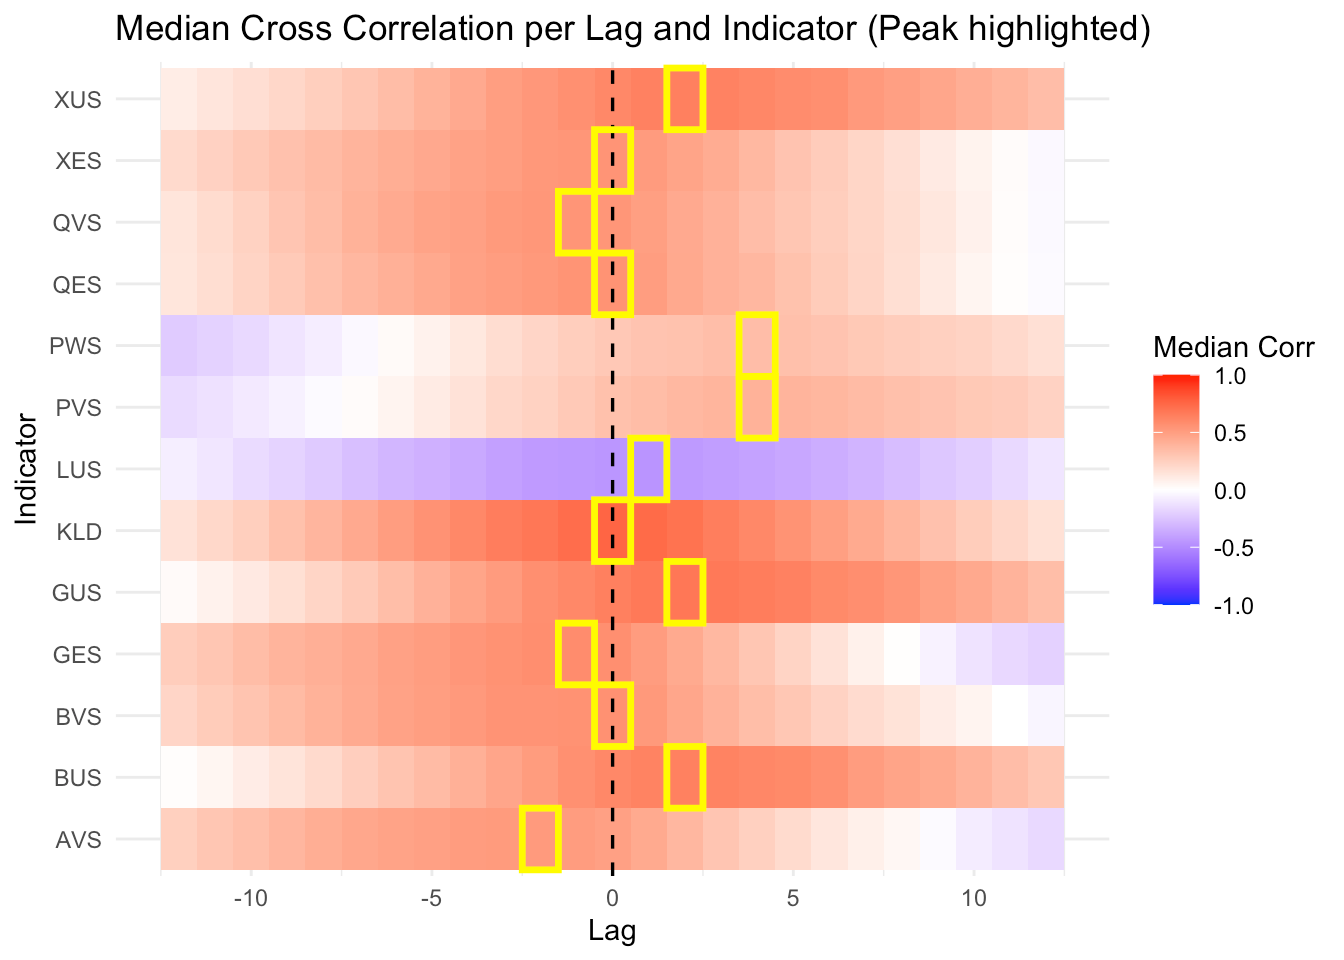
\includegraphics[width=\linewidth]{DominikPlots/as_median_ccf.png}
        \caption{Median cross-correlation profiles across industries.}
        \label{fig:median_ccf}
    \end{subfigure}%
    \hfill
    \begin{subfigure}[t]{0.48\linewidth}
        \centering
        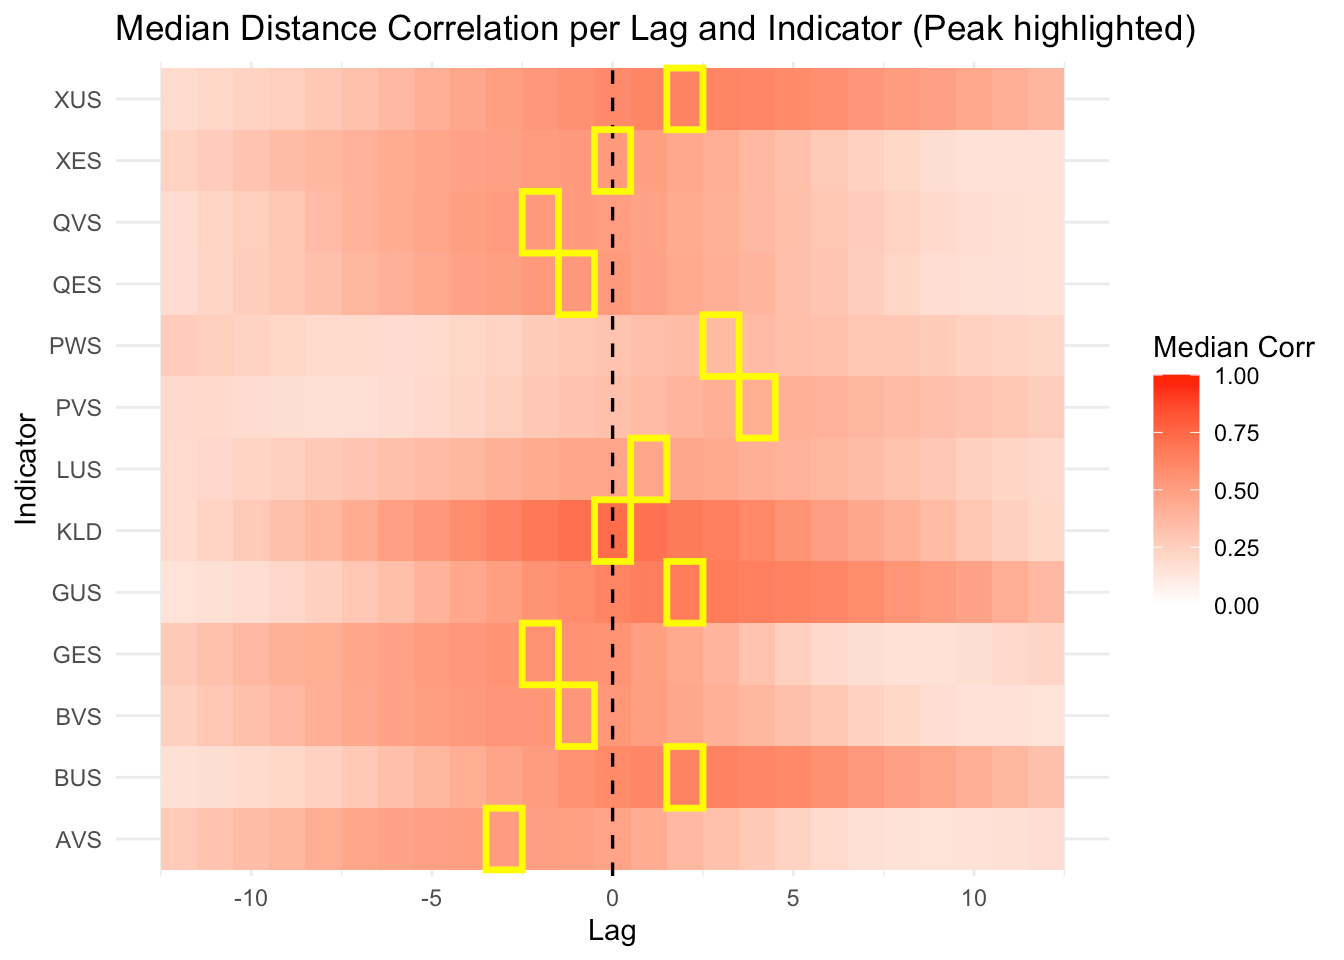
\includegraphics[width=\linewidth]{DominikPlots/as_median_dcor.png}
        \caption{Median distance-correlation profiles across industries.}
        \label{fig:median_dcor}
    \end{subfigure}
    \caption{Comparison of median cross-correlation and distance-correlation profiles across industries.}
    \label{fig:correlation_profiles}
\end{figure}


\subsection{Correlation Distribution}
To gain a deeper understanding of the correlation structure between the survey questions and the main index, we analyze the distribution of correlations at the level of individual questions and industry codes. The goal of this exercise is to disentangle how strongly different industries contribute to the aggregate signal, and how stable these relationships are across time, sectors, and hierarchical levels.

Because the central point of interest here is the \textit{strength of dependence}, we focus on distance correlation as the primary metric. Unlike cross-correlation, which emphasizes timing and direction, distance correlation allows us to summarize the overall magnitude of association independently of linearity or lag alignment. This makes it a natural choice for characterizing the distribution of correlations across a large number of industries.

\subsubsection{Correlation Distribution by Time}
From an economic perspective, it is important to assess whether the correlation structure remains stable across different phases of the business cycle, particularly during downturns and periods of stress compared to times of economic expansion. Figure~\ref{fig:cd_ccf_roll} illustrates how average cross-correlations evolve across rolling windows, highlighting both the mean level and the location of peak lags.

\begin{figure}[H]
    \centering
    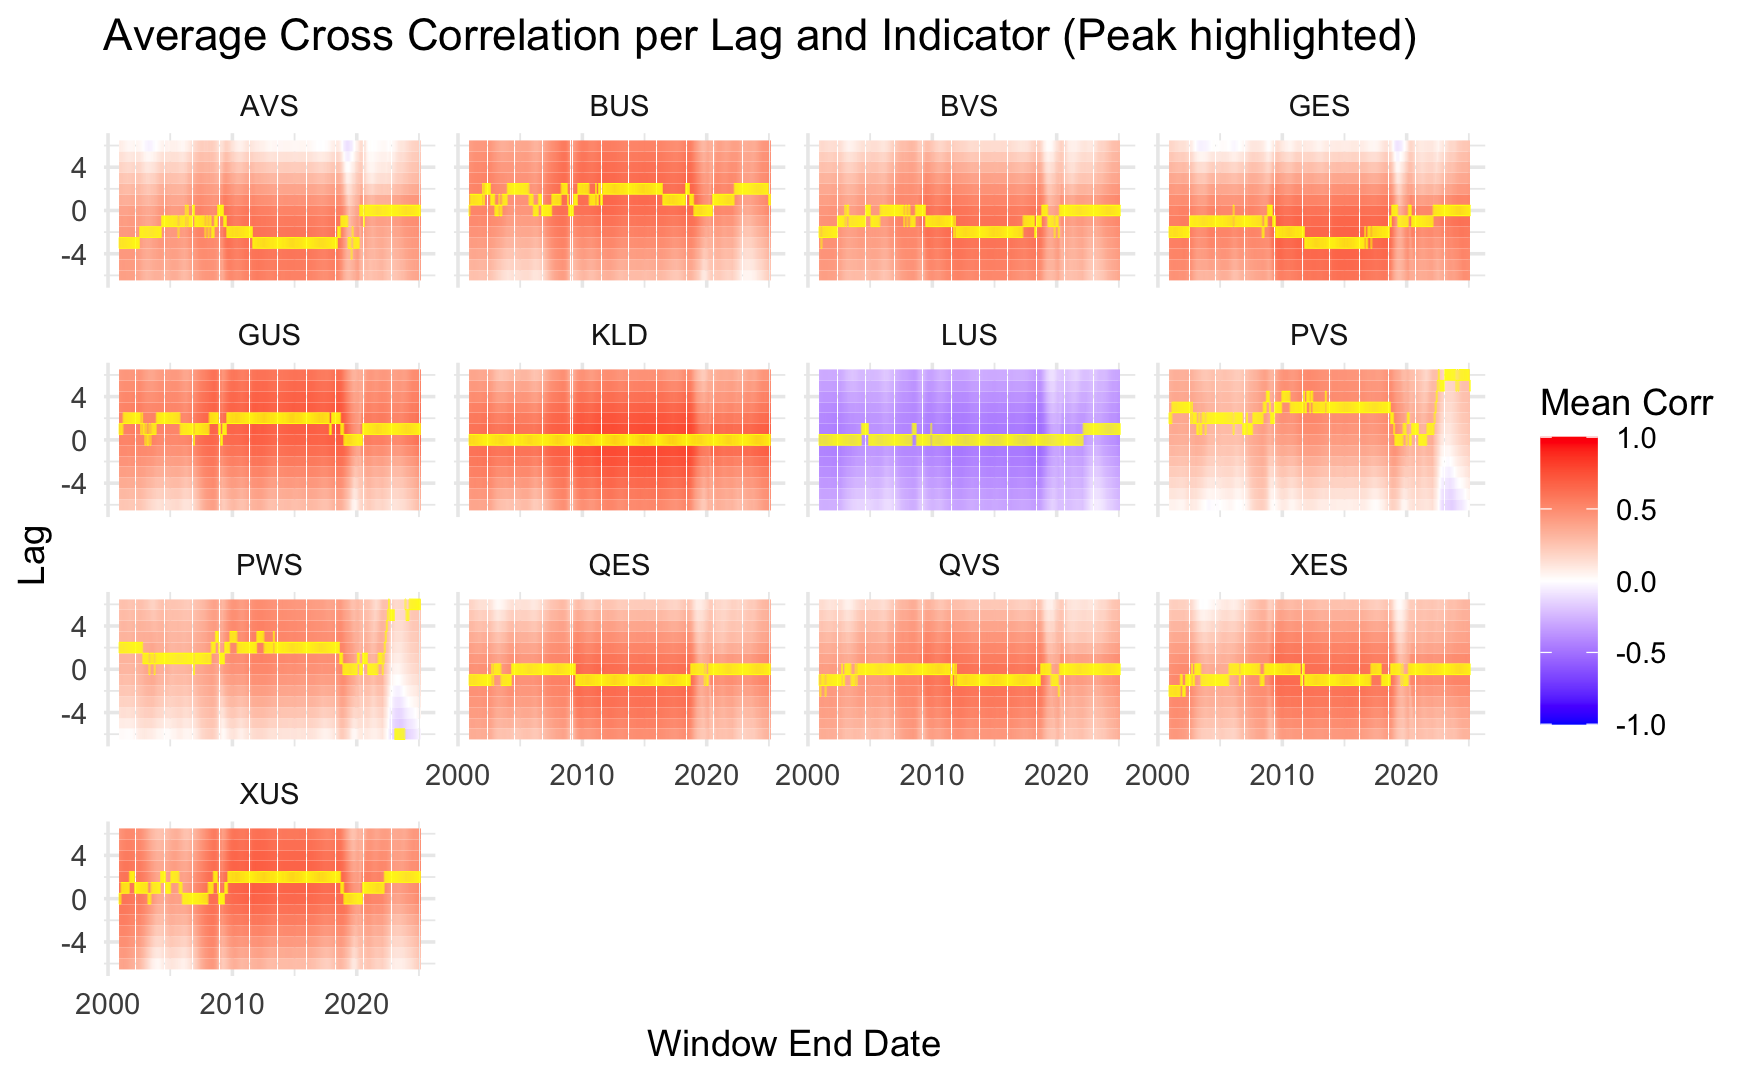
\includegraphics[width=0.7\linewidth]{DominikPlots/cd_ccf_roll.png}
    \caption{10-year rolling window analysis (1-month step), 2000--2025.}
    \label{fig:cd_ccf_roll}
\end{figure}

Beyond average correlations, it is equally important to study the \textit{distribution} of correlations across industries. Figure~\ref{fig:peak_dcor} presents the development of peak distance correlations over time, disaggregated by question. The figure shows both the median (red line) and the dispersion across industry codes (quantiles), thereby capturing not only the central tendency but also the variance of the dependence structure.

\begin{figure}[H]
    \centering
    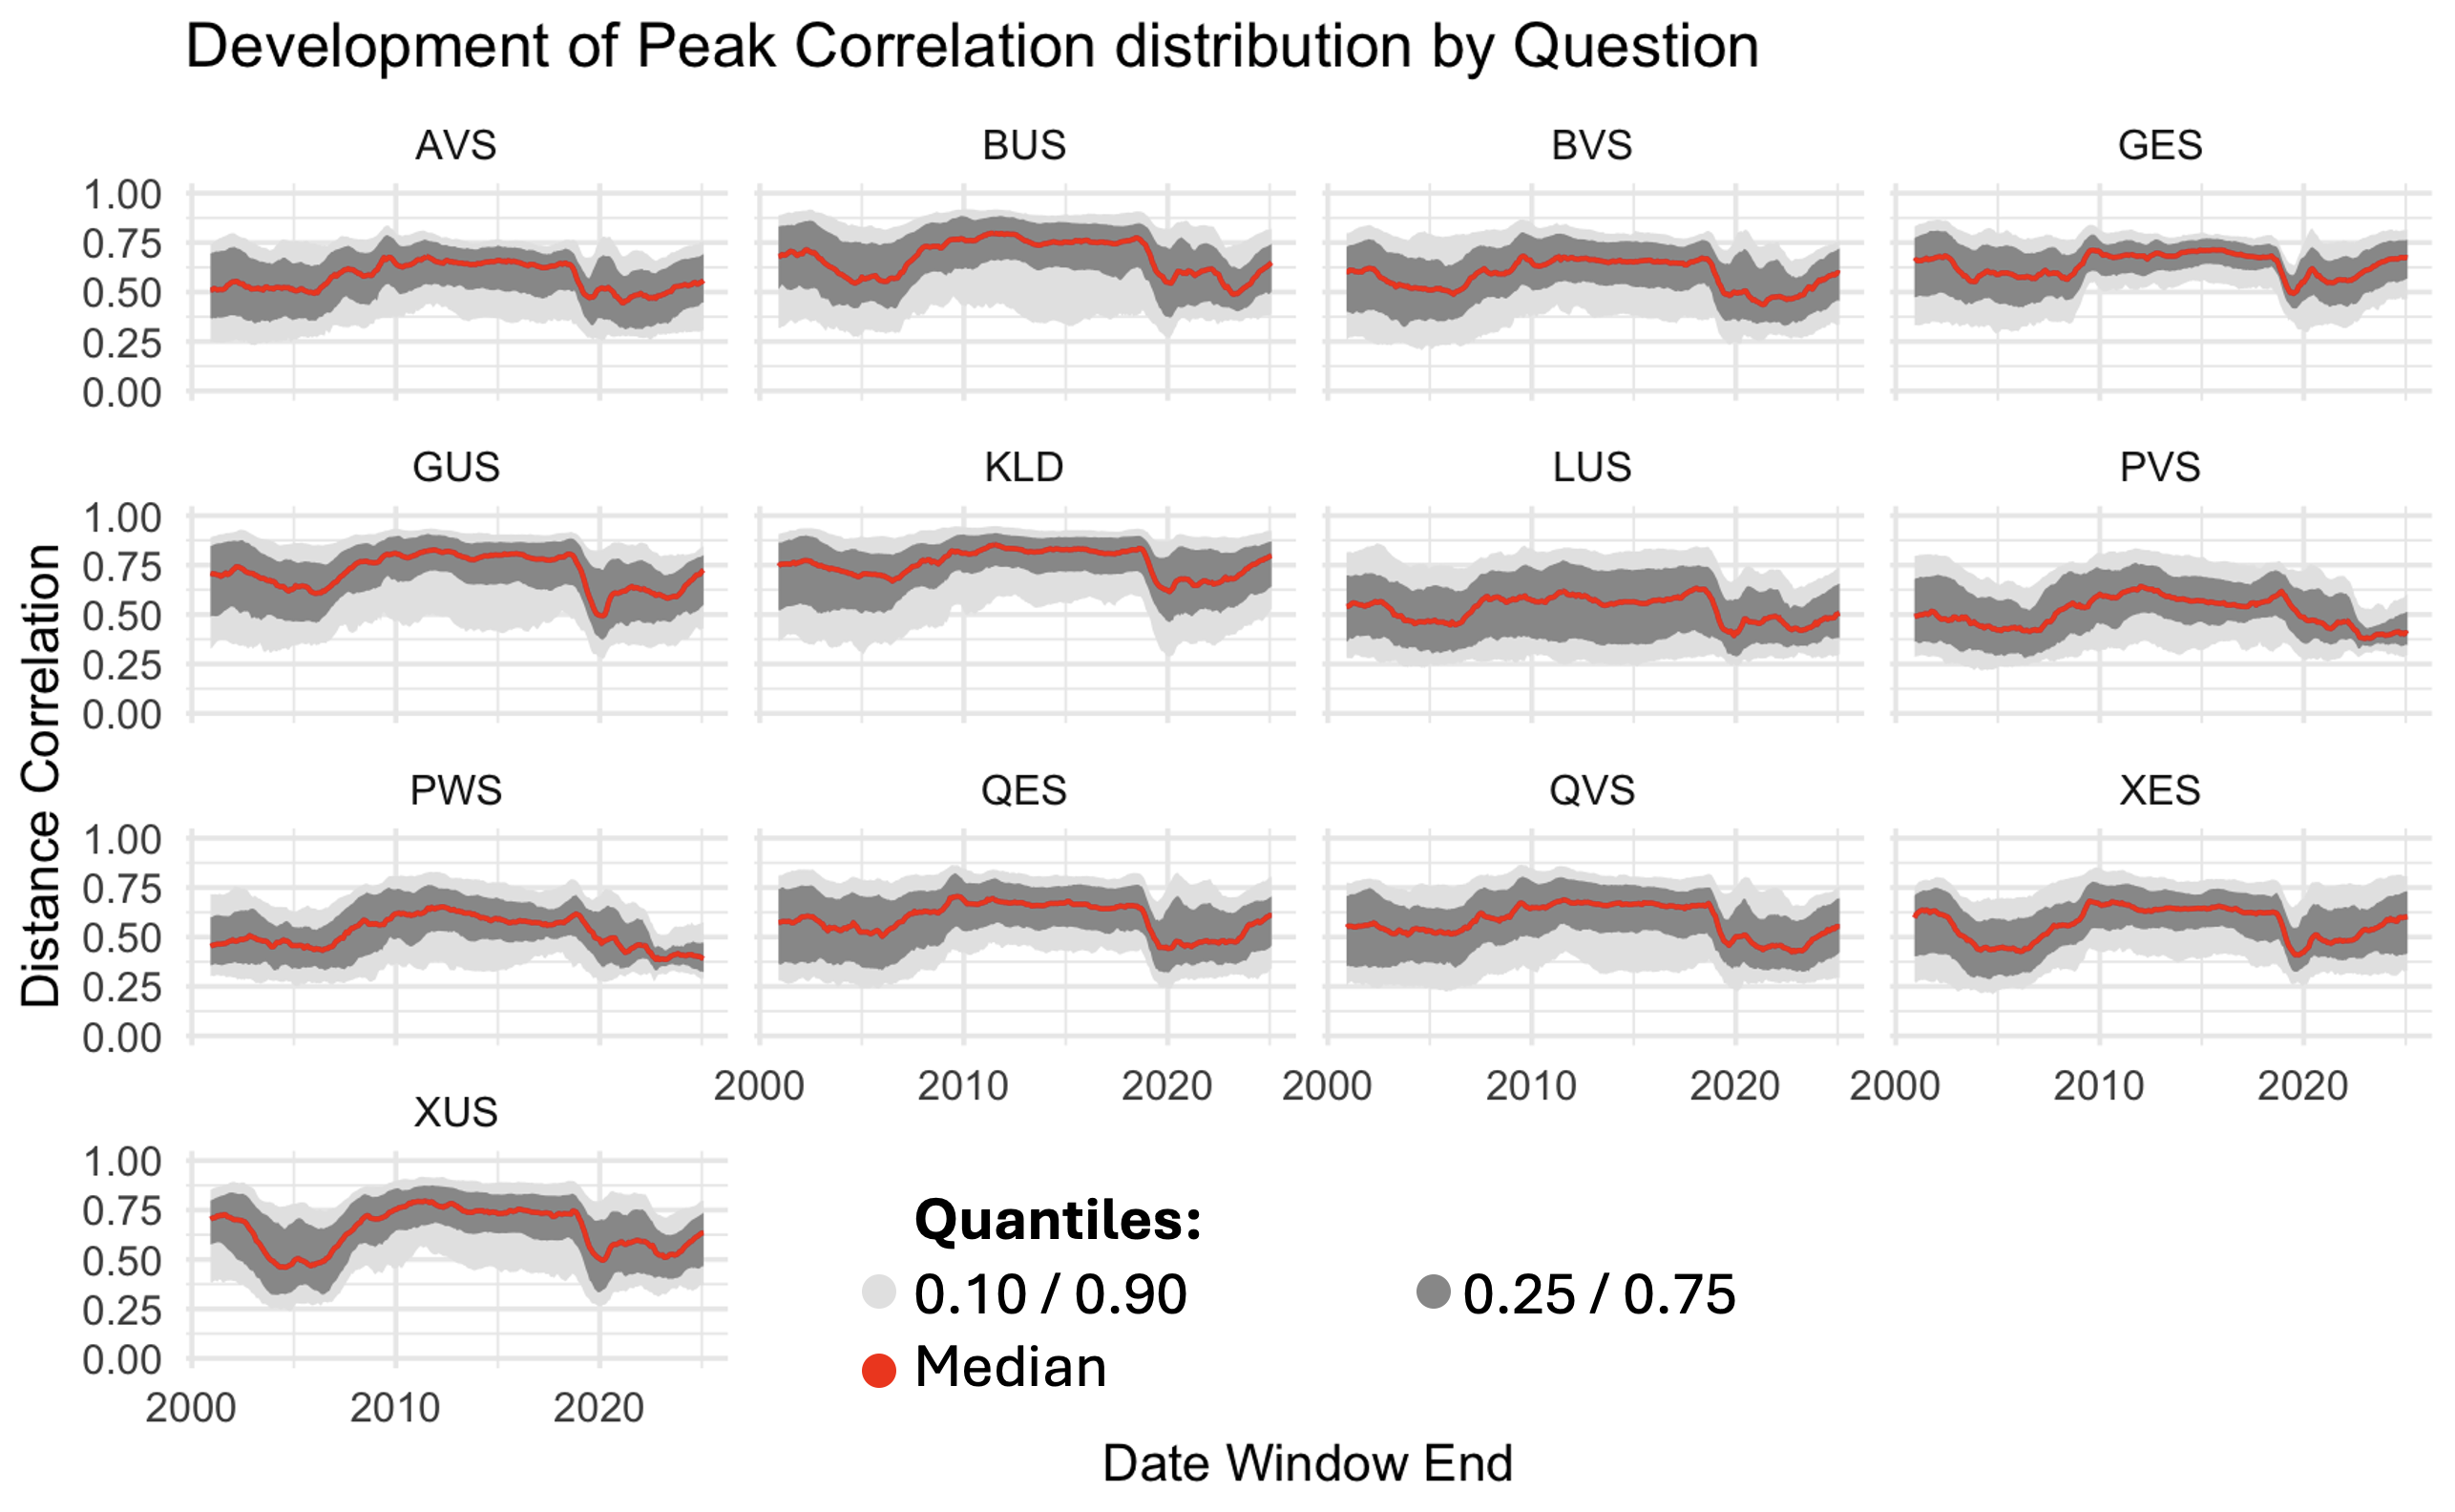
\includegraphics[width=0.7\linewidth]{DominikPlots/cd_dcor_dist_roll.png}
    \caption{Peak distance correlation by question, with median and inter-quantile ranges, Levels 1--3.}
    \label{fig:peak_dcor}
\end{figure}

\vspace{\baselineskip}
\vspace{\baselineskip}
Taken together, these results highlight two important insights. First, the correlation structure exhibits clear breaks around major economic events, most notably the global financial crisis of 2008--2009 and the COVID-19 pandemic after 2018. During these periods, both the level and the dispersion of correlations shift markedly, reflecting heterogeneous responses of industries to systemic shocks. Second, despite these disruptions, the overall correlation structure remains relatively stable in calmer periods, suggesting that the main index captures persistent common dynamics across manufacturing industries. This stability provides reassurance that industry-level correlations can serve as reliable indicators of aggregate developments, while the observed breaks emphasize their usefulness in detecting structural shifts.

\subsubsection{Correlation Distribution by Sector}
Examining the distribution of peak distance correlations at the sector level reveals substantial heterogeneity across industries (Figure~\ref{fig:cd_dcor_dist_sector}). Some sectors exhibit consistently strong correlations with the main index, while others display weaker or more dispersed relationships. This underlines the heterogeneous character of the German manufacturing landscape, where not all industries contribute equally to the aggregate dynamics.

\begin{figure}[H]
    \centering
    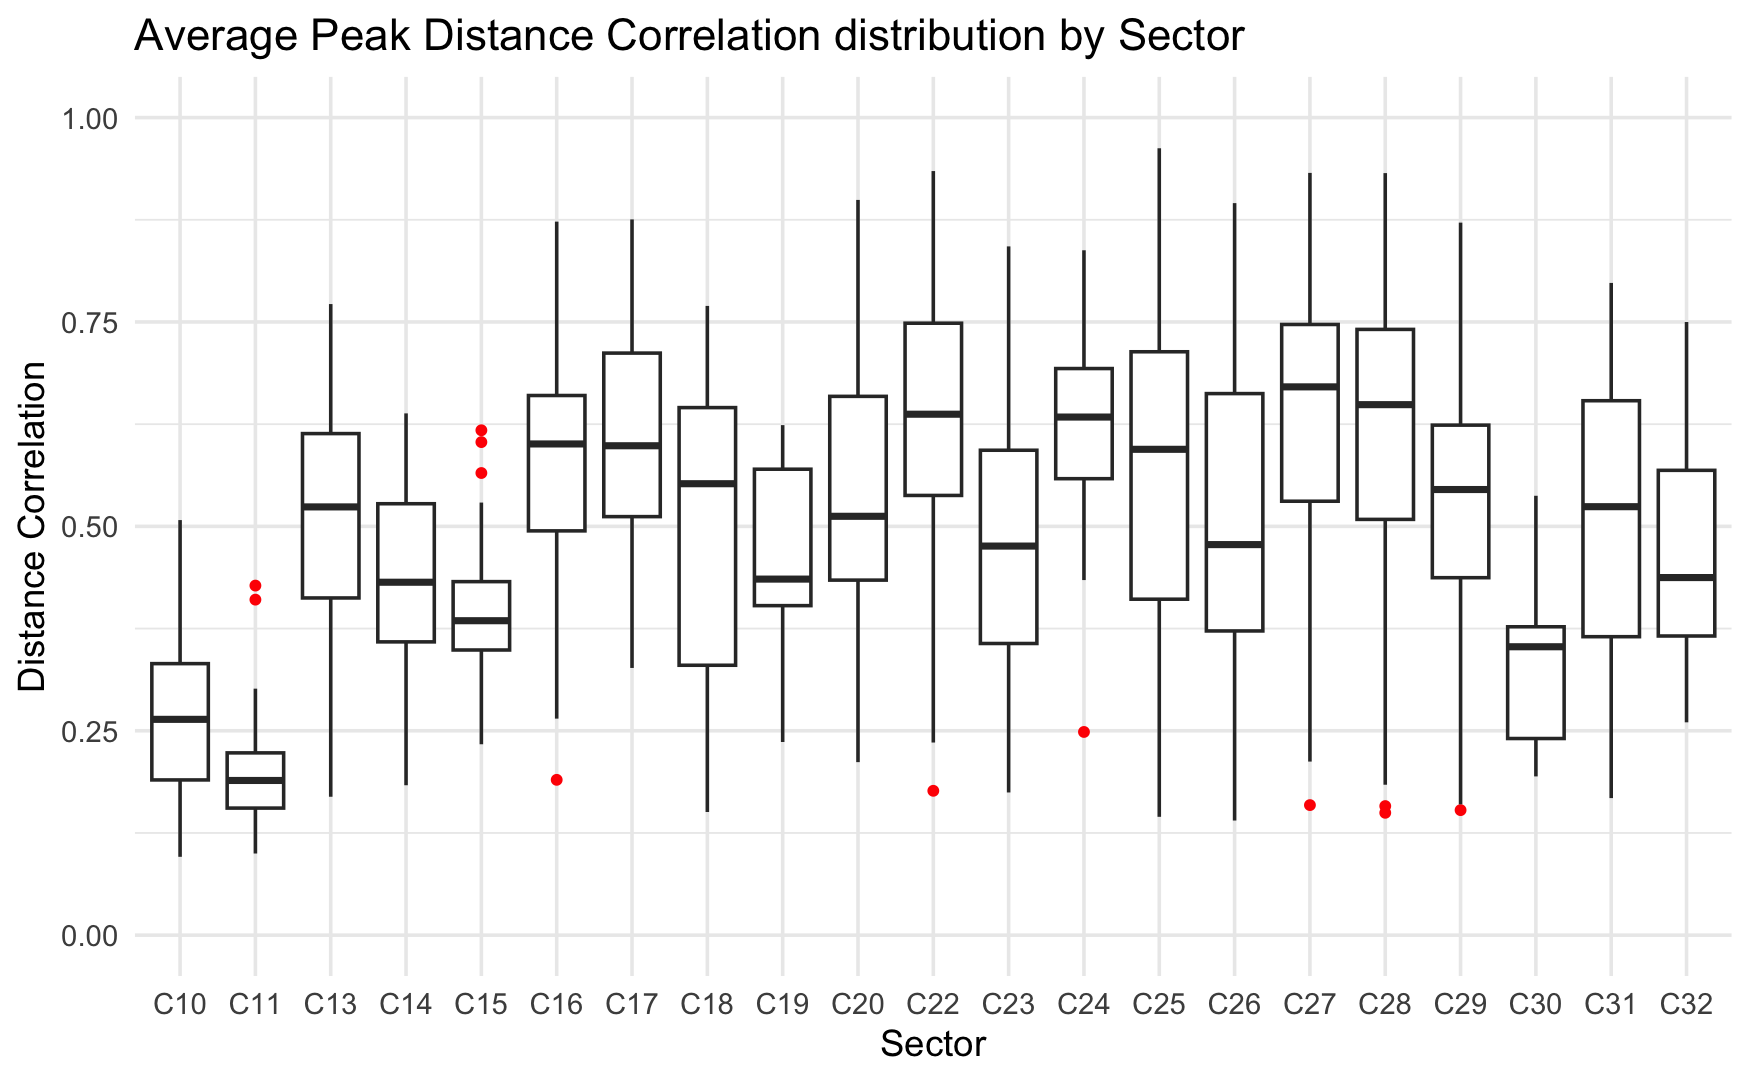
\includegraphics[width=0.7\linewidth]{DominikPlots/cd_dcor_dist_sector.png}
    \caption{Distribution of peak distance correlations by sector.}
    \label{fig:cd_dcor_dist_sector}
\end{figure}

It is important to note that the aggregation underlying the main index is weighted by the economic importance of each sector. As a result, the index successfully reflects overall economic developments, but it does not necessarily mirror the behavior of each individual industry. Certain sectors may therefore play only a limited role in shaping the aggregate signal, even though they are economically relevant in their own right.

From a modeling perspective, these results suggest that the dynamics of the main index can be effectively captured by focusing on a smaller set of industries with consistently strong correlations. Identifying such sectors provides a path towards sparser models that retain explanatory power while avoiding the noise introduced by less strongly aligned industries.


\subsubsection{Correlation Distribution by Level}
As discussed previously, the hierarchical structure of industry codes introduces an inherent imbalance in the number of series across levels. To account for this, we evaluate the correlation distribution separately for the more granular Levels~4--5. Figure~\ref{fig:cd_dcor_dist_level} provides an overview of the distribution of peak distance correlations across levels.

\begin{figure}[H]
    \centering
    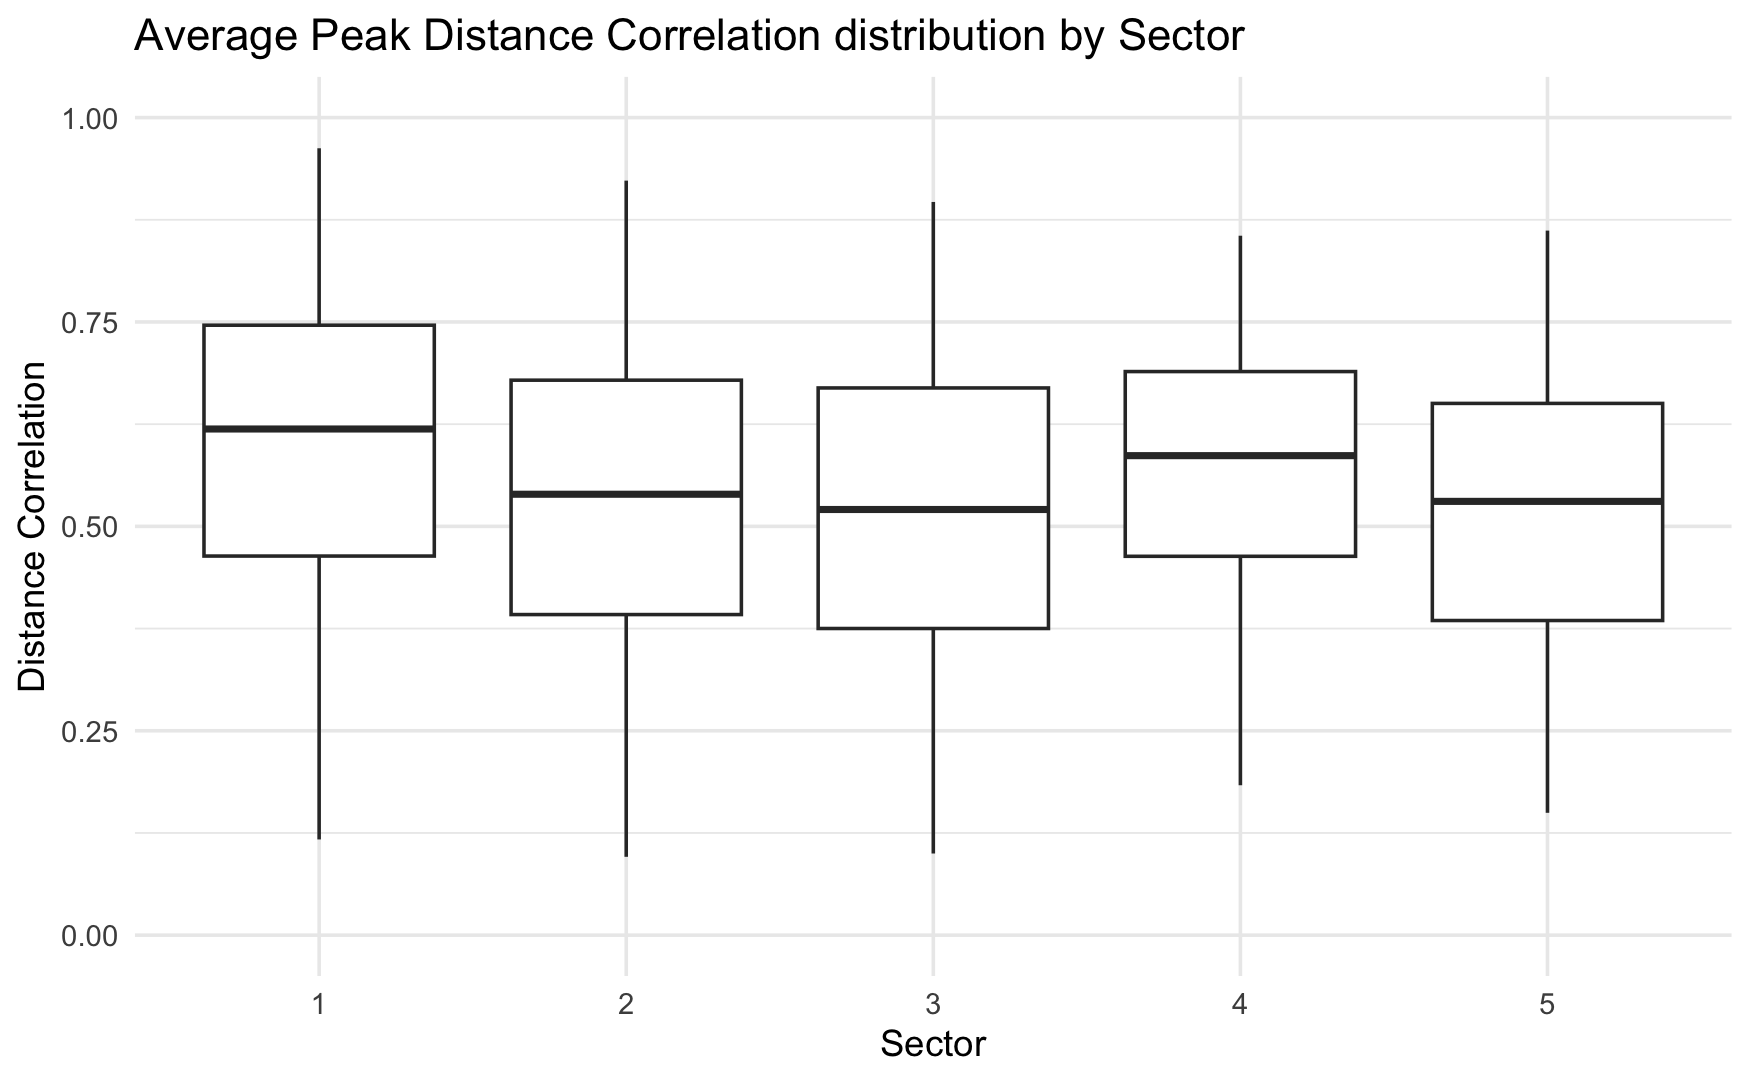
\includegraphics[width=0.7\linewidth]{DominikPlots/cd_dcor_dist_level.png}
    \caption{Distribution of peak distance correlations by hierarchical level.}
    \label{fig:cd_dcor_dist_level}
\end{figure}

The overall picture is that Levels~4--5 exhibit somewhat noisier correlation structures compared to the higher-level aggregations, but they broadly follow the same patterns observed at Levels~1--3. This similarity also extends to their temporal development (Figure~\ref{fig:cd_dcor_dist_roll_level}), where the rolling-window evolution of distance correlations at deeper levels closely tracks that of the broader aggregates. In short, Levels~4--5 appear more volatile, but they remain aligned with the higher-level dynamics.

\begin{figure}[H]
    \centering
    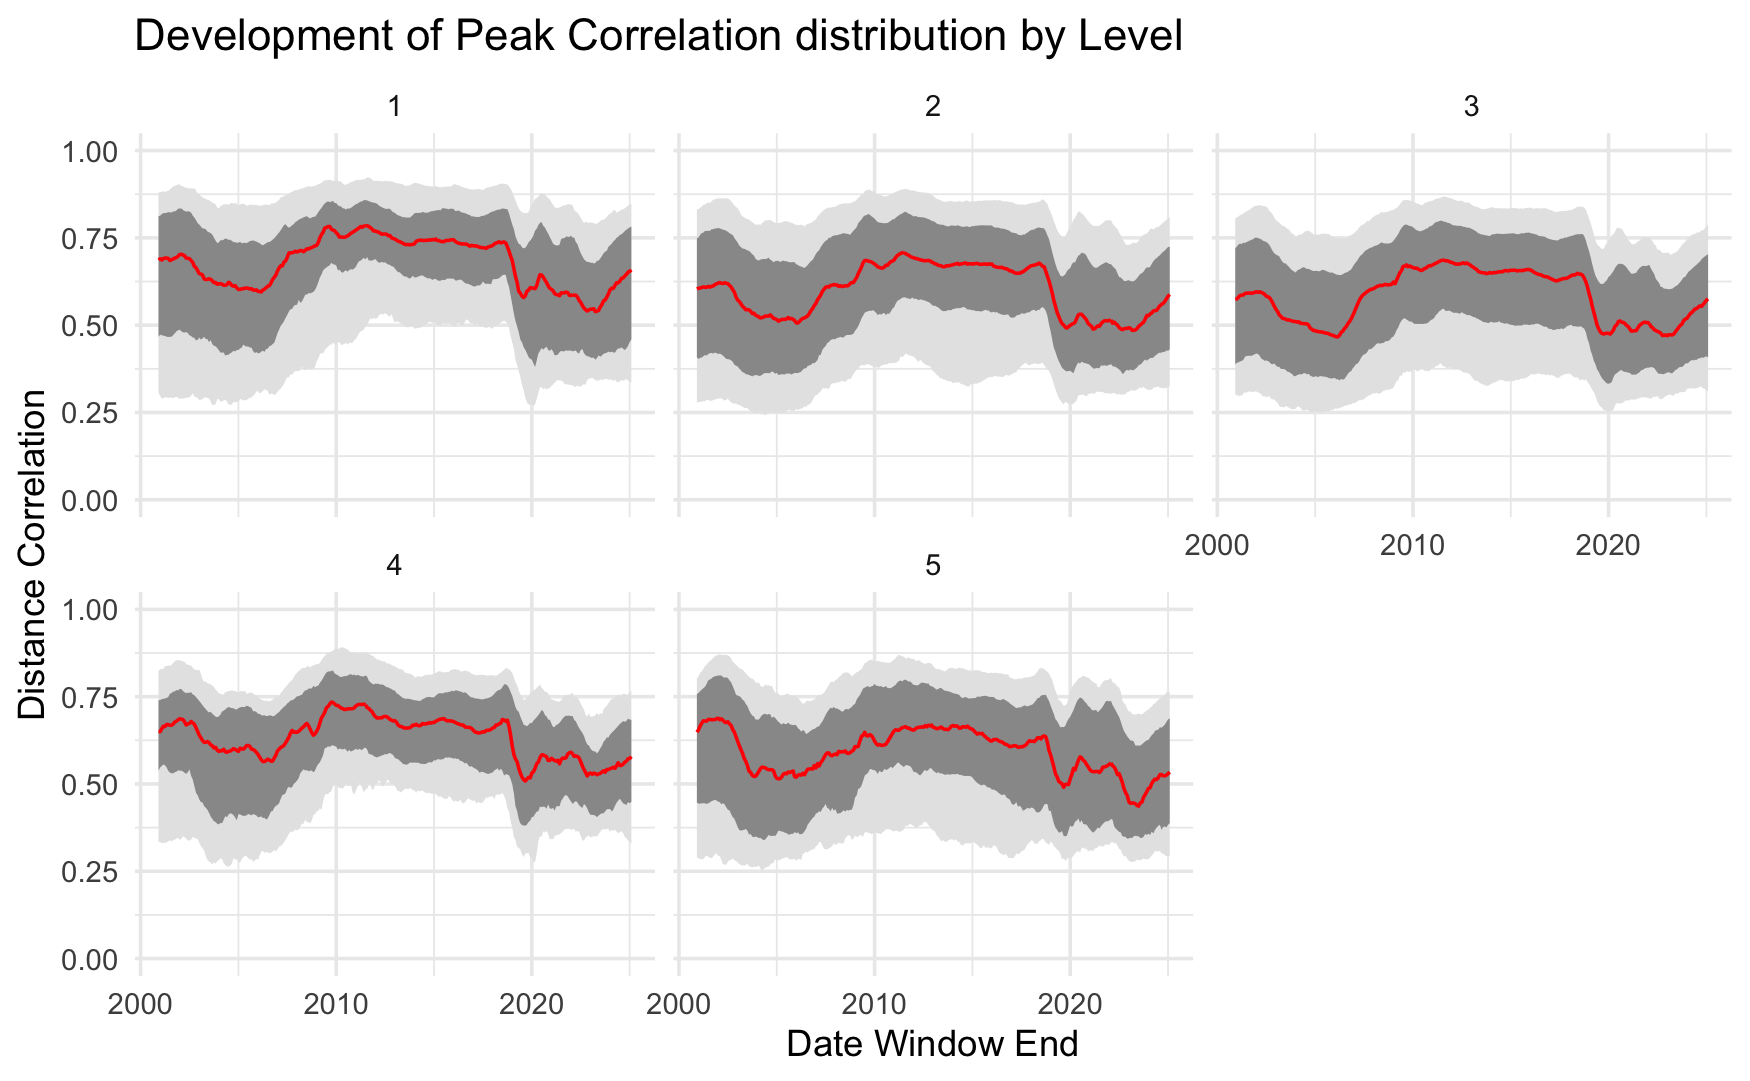
\includegraphics[width=0.7\linewidth]{DominikPlots/cd_dcor_dist_roll_level.png}
    \caption{Rolling-window distribution of peak distance correlations by level.}
    \label{fig:cd_dcor_dist_roll_level}
\end{figure}

From an analytical perspective, this is a noteworthy result. Because Levels~4--5 represent more disaggregated industries, their economic weight in the main index is much smaller than that of Level~1 or Level~2 sectors. Their alignment with the aggregate development is therefore not necessarily the result of construction, but likely reflects genuine causal links to overall business cycle dynamics. This suggests that lower-level industries may serve as a valuable indicative set for monitoring economic developments. Further investigation of these fine-grained series could thus provide useful insights into early signals of aggregate turning points.


\subsection{Consensus Analysis}
In the previous section we examined the variance of correlations across industries, which showed how strongly the dependence structure fluctuates over time. However, this analysis did not reveal whether the relative position of individual industries within the correlation structure remains stable or changes substantially. To address this, we introduce a ranking-based consensus analysis that evaluates the stability of industry rankings across time windows.

The idea is to compare, for each survey question and time window, the set of top-$k$ most strongly correlated industries.\footnote{Throughout the analysis we use $k=30$. This choice reflects a balance between capturing enough of the correlation structure and avoiding excessive noise from lower-ranked industries; robustness checks with alternative $k$ confirmed that the dynamics are well represented at this threshold.} By focusing on the overlap of these top-ranked industries, we can track whether the “core set” of highly correlated industries remains consistent or whether entirely new industries enter the picture over time.

To quantify this, we compute the Jaccard index between two sets $A$ and $B$ of top-$k$ industries:  
\[
  J(A,B) = \frac{|A \cap B|}{|A \cup B|} 
  = \frac{|A \cap B|}{2k - |A \cap B|},\footnote{The second equality holds only because both sets $A$ and $B$ are of equal size $k$. In the general case, the denominator is $|A \cup B|$ without simplification.}
\]
The Jaccard index ranges from $0$ (no overlap) to $1$ (perfect overlap), and thus measures how similar the top-$k$ sets are across windows. Averaging these pairwise values over time yields a nonlinear consensus metric that captures the overall stability of the ranking structure.

\begin{figure}[H]
    \centering
    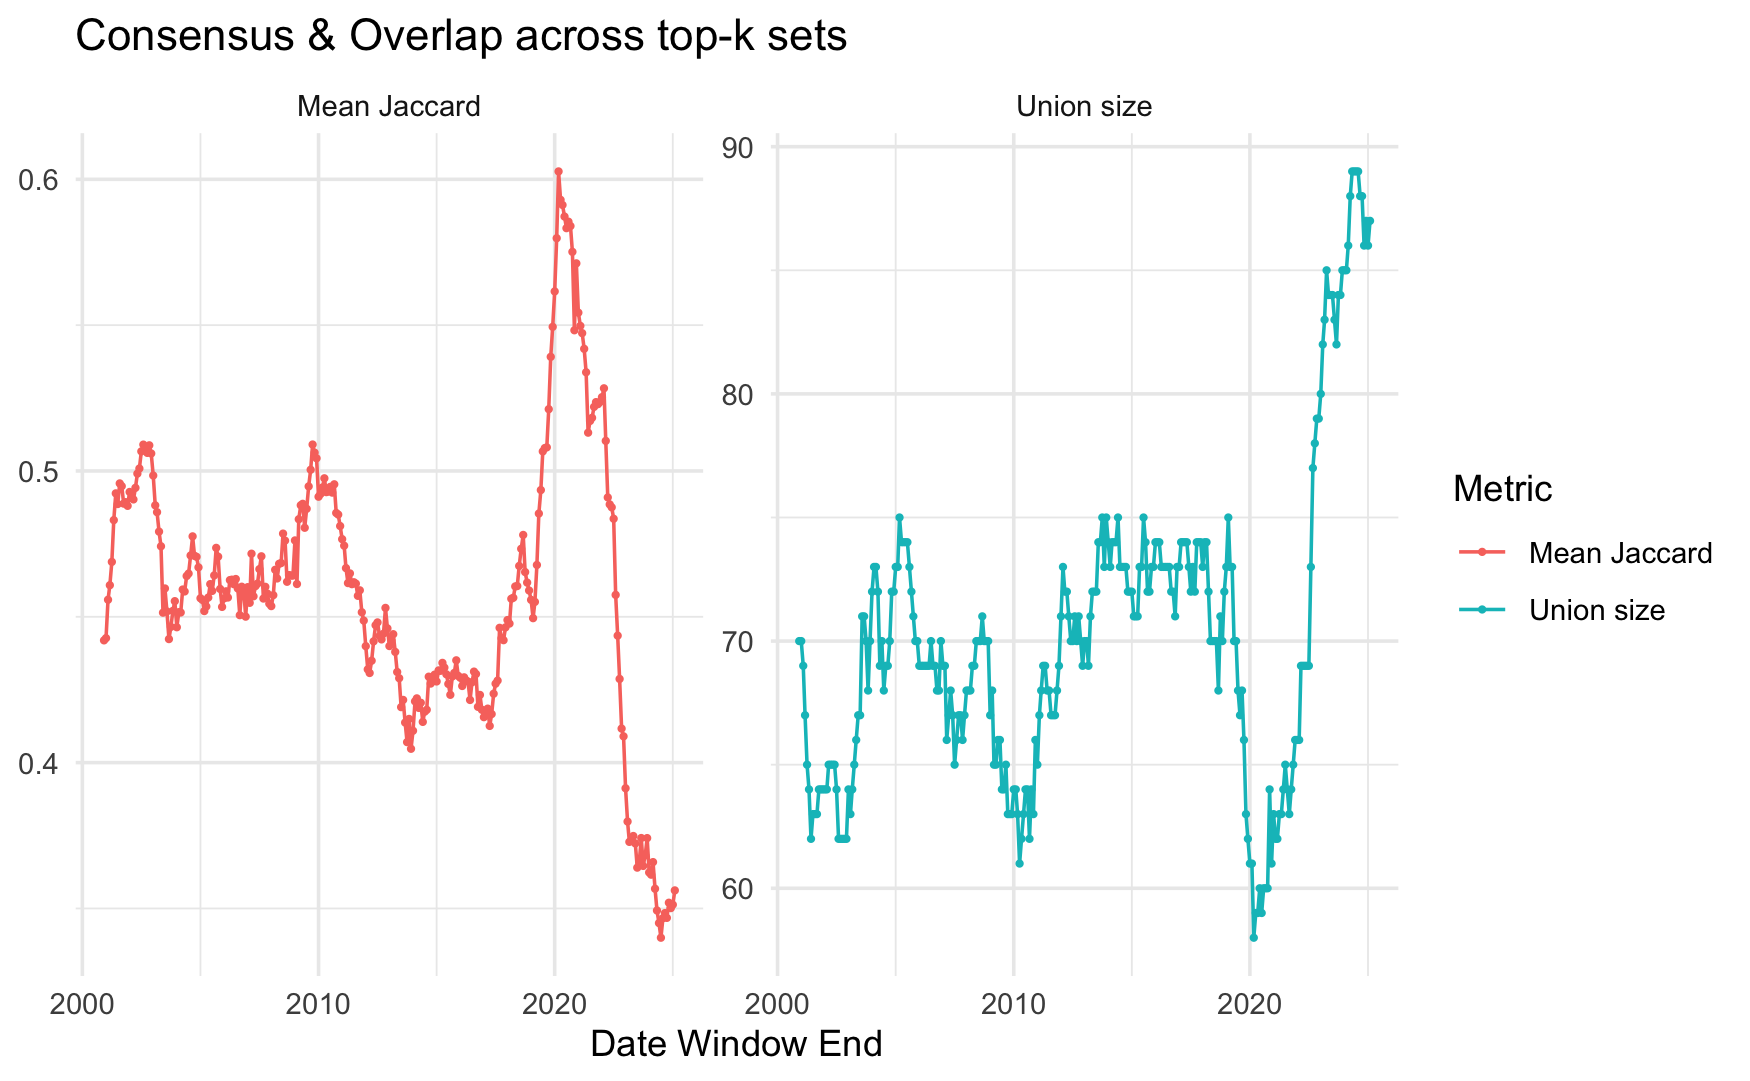
\includegraphics[width=0.7\linewidth]{DominikPlots/ca_jaccard_union.png}
    \caption{Consensus of top-30 sets (Jaccard index) vs.\ union size over time.}
\end{figure}

The results reveal two important features. First, higher average Jaccard values combined with smaller union sizes indicate that the structure is increasingly dominated by a relatively small group of industries, i.e., the same industries repeatedly occupy the top ranks. Second, we observe sharp spikes in consensus around major economic events. The strongest such spike occurs in 2020 during the COVID-19 pandemic, exceeding those seen during earlier crises such as the dot-com downturn in 2002 or the global financial crisis in 2008–2010. This pattern suggests that systemic shocks compress the correlation structure, temporarily aligning industries more closely than in normal times.

From an economic perspective, this alignment provides valuable information: during crises, the set of industries that best track the main index becomes more homogeneous, while in stable periods the ranking is more dispersed. In other words, systemic stress appears to “synchronize” industry-level dynamics. This observation points to the potential of consensus analysis as a diagnostic tool: sharp increases in consensus may serve as early signals of widespread economic stress. Further research should investigate whether such consensus spikes can be systematically linked to the onset of recessions or other structural breaks.

%---------------
\newpage
%--------------------------------------------------------------------------------
-----------------------------------------------------------------
\section{Granger Causality}
\label{ch:granger causallity}

\subsection{Methodology}

\subsubsection{Motivation and Definition}
This section moves beyond simple correlation to investigate linear predictive relationships between industry-specific time series and the main index. In particular, we are interested in finding industries that are "causing" the main index. Ideally, a cause should happen before its effect. Additionally, a cause should provide unique information about the future values of the effect. Finding such industries would enable us to forecast the main index. Similar considerations lead the economist Clive Granger to introduce the concept of "Granger Causality". Mathematically this is formalized by \citet{granger1969investigating} in the following way:

\begin{defn}
Let $X$,$Y$ be time-series. $X$ is said to (simple) Granger-cause $Y$ iff.    
\[
\mathrm{Var}\!\left(Y_{t+1}\middle| Y_t,\ldots,Y_1\right) \; > \; \mathrm{Var}\!\left(Y_{t+1}\middle| Y_t,\ldots,Y_1,X_t,\ldots,X_1\right)
\]
We speak of instantaneous Granger Causality iff. \[
\mathrm{Var}\!\left(Y_{t+1}\middle| Y_t,\ldots,Y_1\right) \; > \; \mathrm{Var}\!\left(Y_{t+1}\middle| Y_t,\ldots,Y_1,X_{t+1},\ldots,X_1\right)
\]

\end{defn}

\textbf{Note:} Granger causality does not claim “true” or “philosophical” causality. Instead, it identifies predictive causality, a directional and temporal relationship in which one variable systematically precedes and improves forecasts of another.

\subsubsection{Testing for Granger Causality}
To test for Granger causality, the standard approach is to compare the predictive performance of two nested linear models. First, the dependent variable $Y_t$ is regressed on its own past values up to a chosen lag order (auto-regressive model). Second, an extended model is estimated in which lagged values of another variable $X_t$ are included in addition to the lagged values of $Y_t$. If the inclusion of $X_t$ significantly improves the model’s explanatory power, then $X$ is said to Granger-cause $Y$.


Formally, the null hypothesis states that the lagged values of X do not improve the prediction of Y. The hypothesis is tested by comparing the restricted and unrestricted models using an F-test on the lagged X coefficients. If the null hypothesis is rejected at the chosen significance level, evidence for Granger causality is established. In practice, we use 5\% as the significance level for the hypothesis test and a fixed number of lags (between 1 and 6). We use the standard \textit{anova}-function from R to perform the hypothesis test.



\subsection{Results}

\subsubsection{Instantaneous Granger Causality}
We start our analysis with instantaneous Granger Causality as this concept has been longer established.
\newline

\textbf{Test with single survey question} 
\newline
The analysis was performed on every single industry classified in level 2 and level 3. For each industry, we tested the relationship between individual survey questions and the main index, applying a range of time lags from one to six periods. This multi-lag approach ensures that we capture both immediate and delayed relationships between the variables.

\begin{itemize}
    \item \textbf{Level 2}: For all 50 industries within this classification, we found that at least one survey question was instantaneous Granger Causal to the main index. This universal result at a broader industry level highlights a consistent predictive link.
    \item \textbf{Level 3}: The findings were similarly robust at the more granular level 3. Of the 61 industries analyzed, 60 demonstrated that at least one survey question was Granger Causal to the main index.
\end{itemize}





Identified Exception: A single exception was noted. The industry C2529000 - "Manufacture of containers" was the only one that did not show a Granger Causal relationship with the main index within the tested parameters.
\newline






\textbf{Significant Survey Questions} 
\newline
Given that most industries show a predictive relationship with the main index, we next identify the specific survey questions that are the most consistent and powerful predictors.. By examining the distribution of instantaneous Granger Causality across all questions, we can determine which questions are most appropriate for use in forecasting models.

\begin{figure}[H]
    \centering
    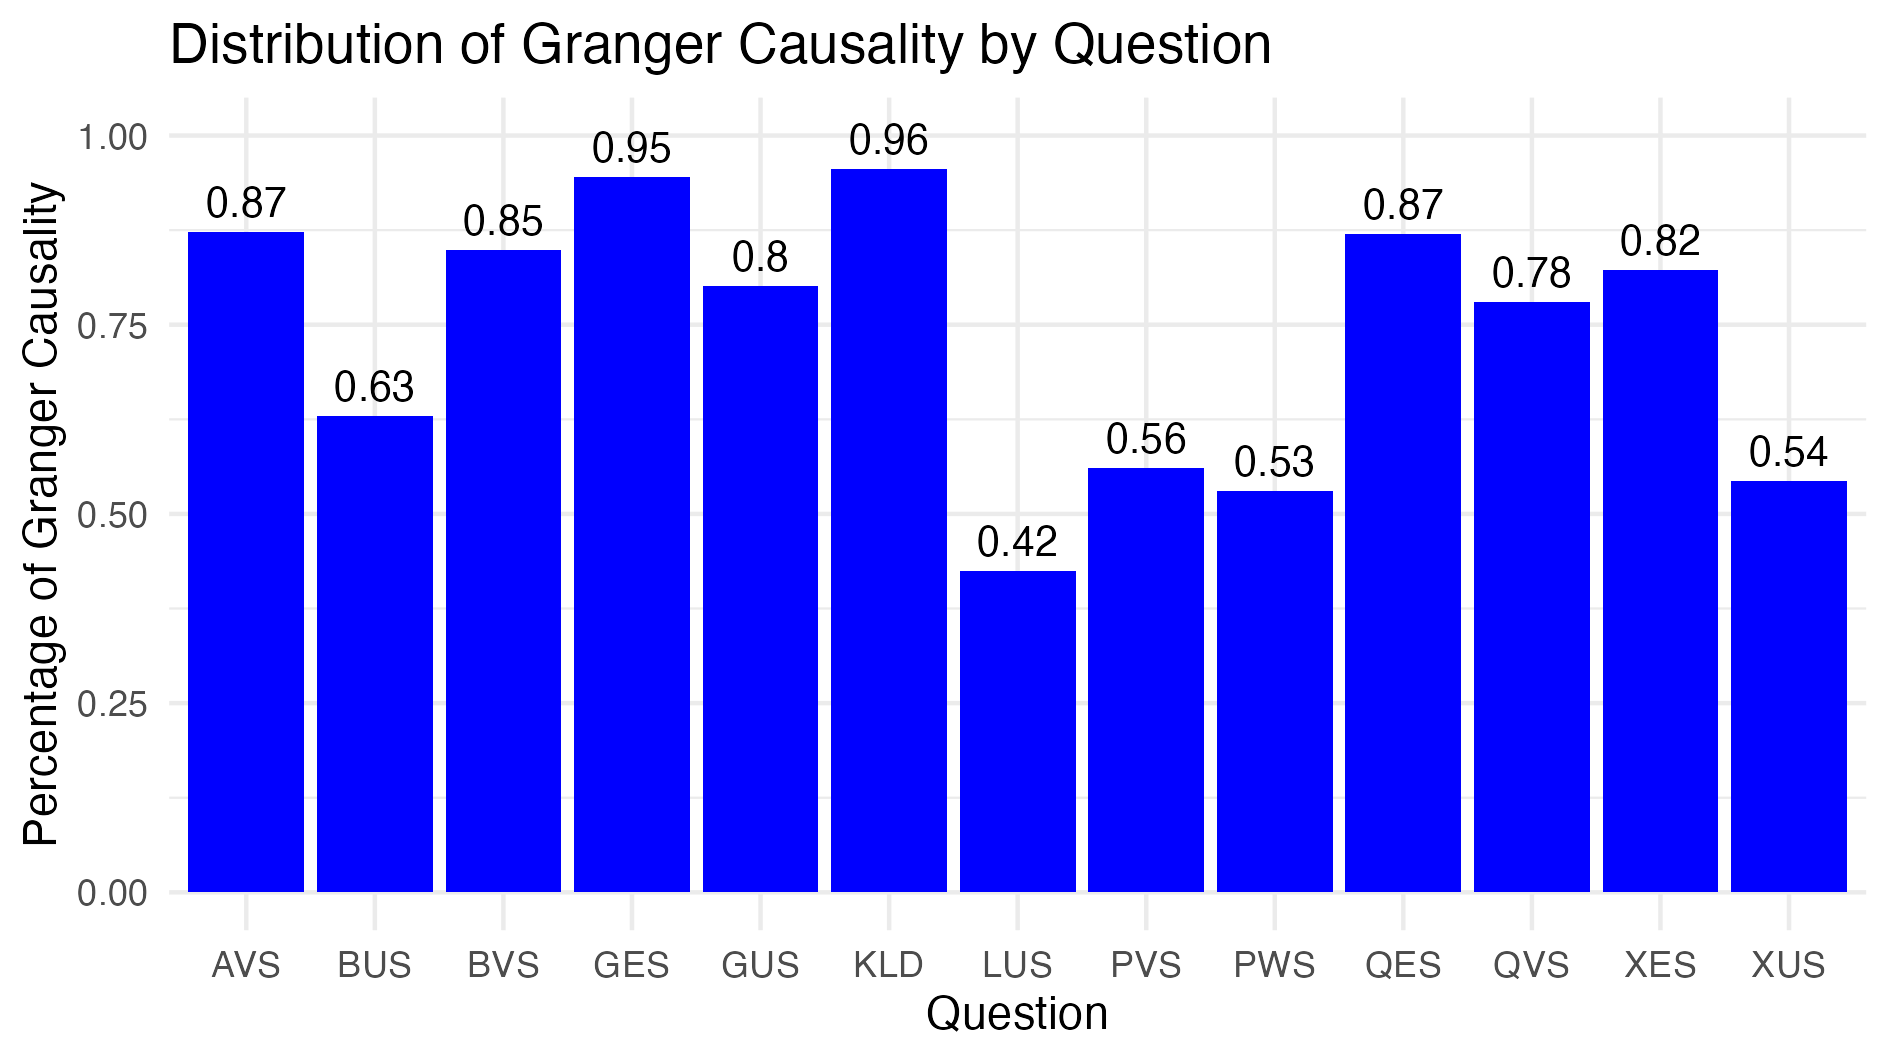
\includegraphics[width=0.9\textwidth]{DanielPlots/distribution_gc_questions_instantaneous.png}
    \caption{Distribution across questions indicating instantaneous Granger causality.}
\end{figure}

The key observations from the data are as follows:

\begin{itemize}
    \item Strongest Predictors: A few questions stand out as exceptionally reliable. The question abbreviated as KLD shows a instantaneous Granger Causal relationship in 96\% of the industries tested, followed closely by GES at 95\%. Other strong performers include AVS and QES, both at 87\%. These questions consistently provide predictive information across the vast majority of industries.

    \item Weaker Predictors: Not all questions carry the same predictive weight. The question LUS was found to be instantaneous Granger Causal in only 42\% of industries, making it the least reliable predictor in this analysis. Other questions like PVS (56\%) and PWS (53\%) are also comparatively weaker, though still predictive for a majority of industries.
\end{itemize}












\textbf{Magnitude of information gain}
\newline
To quantify the marginal contribution of industry-specific data to the performance of the forecasting model, the adjusted $R^2$ was used as the evaluation metric. The adjusted $R^2$ is utilized to determine the proportion of variance in the aggregate index that is explained by the model, adjusting for the number of predictors. The "information gain" from incorporating industry-specific data was calculated as the delta in adjusted $R^2$ between a full model containing the industry data and a reduced baseline model without it. The analysis revealed a maximum increase in adjusted $R^2$ of only 0.0212, associated with the 'Manufacture of non-industry-specific machinery' sector and it's business climate (KLD) question. This demonstrates that the marginal information gain from any single industry's data is negligible.
\begin{figure}[H]
    \centering
    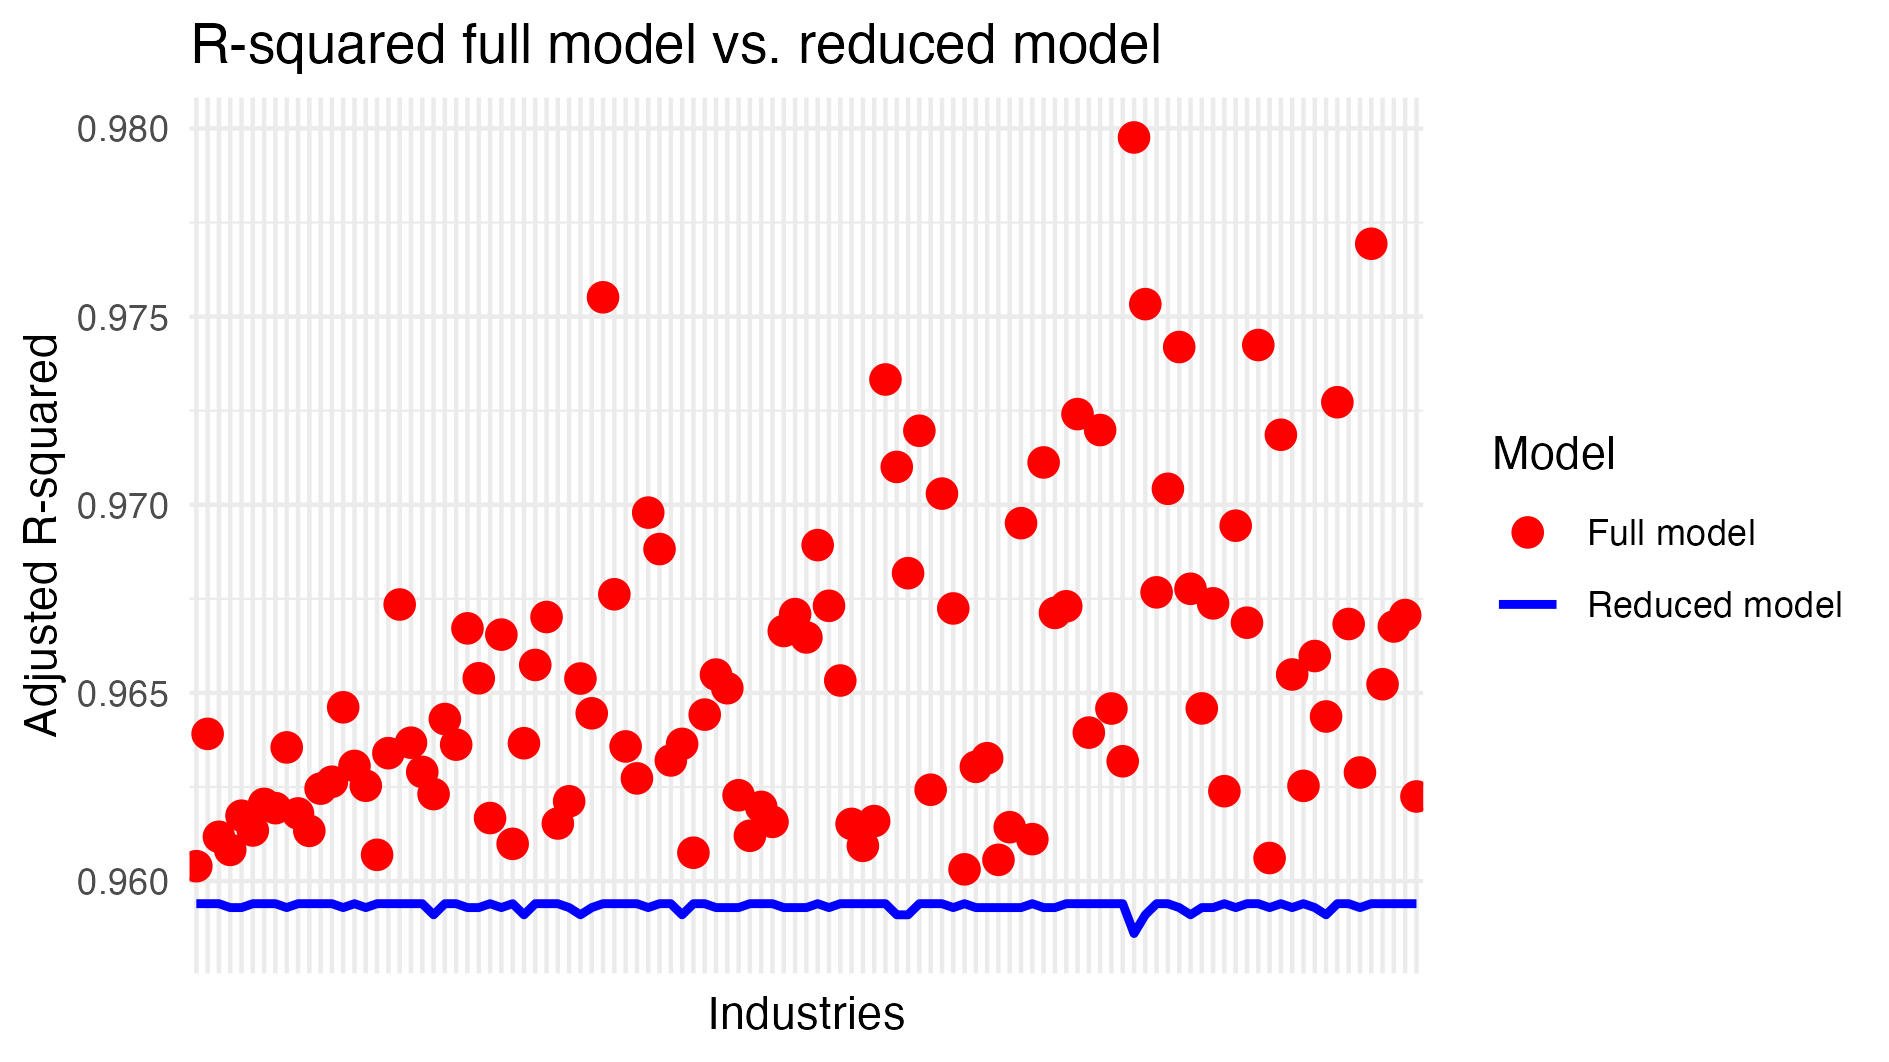
\includegraphics[width=0.9\textwidth]{DanielPlots/adj_r2_plot_instantaneous.png}
    \caption{Adjusted $R^2$ differences (univariate).}
\end{figure}



\renewcommand{\arraystretch}{1.3}
\begin{table}[H]
\centering
\begin{tabularx}{\textwidth}{X c c c}
\toprule
\textbf{Industry} & \textbf{Question} & \textbf{Lag} & \textbf{diff. adj. $R^2$} \\
\midrule
Manufacture of non-industry-specific machinery & Business climate & 3 & 0.0212 \\
Manufacture of parts and accessories for motor vehicles & Business climate & 5 & 0.0175 \\
Manufacture of plastic products & Business climate & 5 & 0.0161 \\
Manufacture of non-specialised machinery & Business climate & 6 & 0.0149 \\
Manufacture of machinery for other specific industries & Business climate & 5 & 0.0148 \\
\bottomrule
\end{tabularx}
\caption{Top 5 industries by difference in adjusted $R^2$ (univariate).}
\end{table}


Using all questions as covariates improves $R^2$, but the same industries dominate.

\renewcommand{\arraystretch}{1.3}
\begin{table}[H]
\centering
\begin{tabularx}{\textwidth}{X c c}
\toprule
\textbf{Industry} & \textbf{Lag} & \textbf{diff. adj. $R^2$} \\
\midrule
Manufacture of non-industry-specific machinery & 2 & 0.0247 \\
Manufacture of plastic products & 4 & 0.0224 \\
Manufacture of parts and accessories for motor vehicles & 6 & 0.0217 \\
Manufacture of machinery for other specific industries & 6 & 0.0204 \\
Manufacture of non-specialised machinery & 3 & 0.0191 \\
\bottomrule
\end{tabularx}
\caption{Top 5 industries by difference in adjusted $R^2$ (multivariate).}
\label{tab:top5_diff_adj_r2}
\end{table}

Visually, the business climate index for the 'Manufacture of Non-industry-specific machinery' sector exhibits a high correlation with the aggregate index but displays significantly greater amplitude in its cyclical fluctuations, with more pronounced peaks and troughs.

\begin{figure}[H]
    \centering
    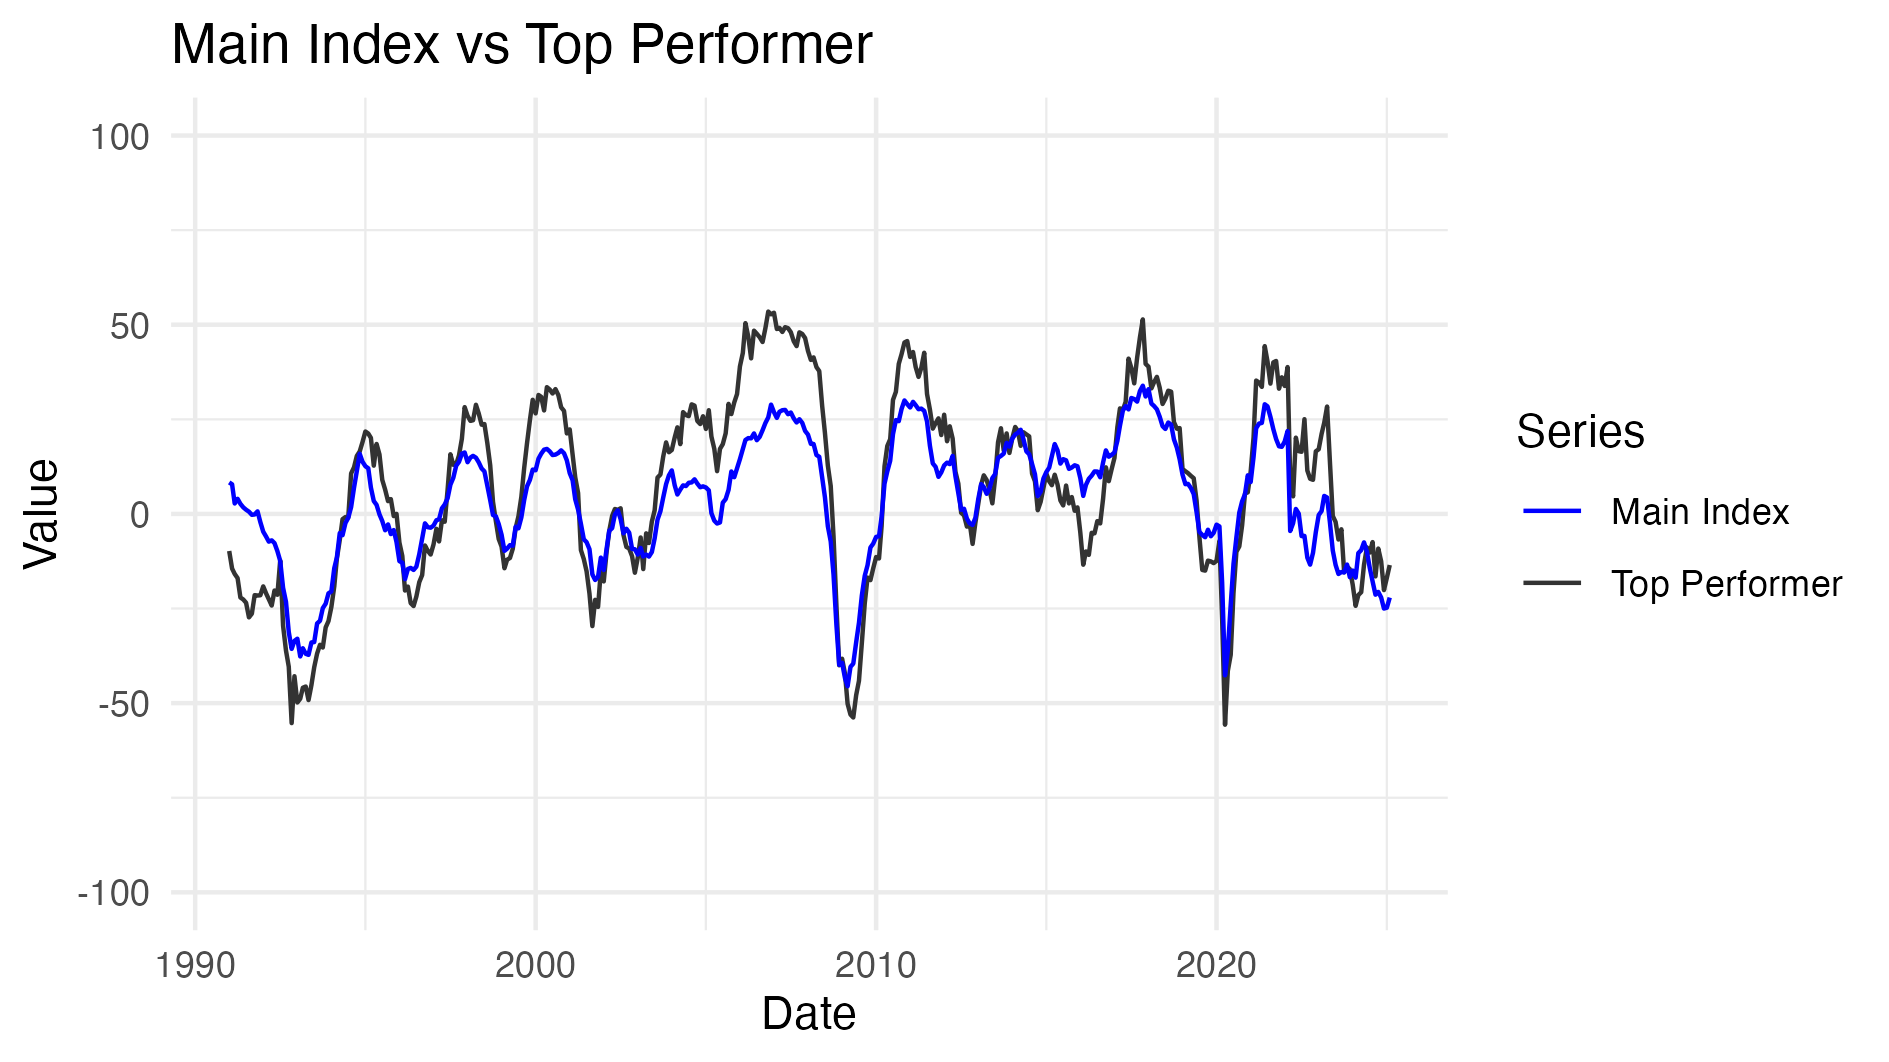
\includegraphics[width=\textwidth]{DanielPlots/main_vs_top.png}
    \caption{Main index vs.\ top-performing industry}
\end{figure}






\subsubsection{Simple Granger Causality}

Similar to the instantaneous case, the same analysis was also performed for simple Granger Causality on every single industry classified in level 2 and level 3. For each industry, we tested the relationship between individual survey questions and the main index, applying a range of time lags from one to six periods. For brevity we will highlight only the differences to instantaneous causality.
\newline





\textbf{Test with single survey question} 



\begin{itemize}
    \item \textbf{Level 2:} Only 48 out of 50 industries have at least
    one survey question that is Granger Causal to the main index.
    \item \textbf{Level 3:} Only 56 out of 61 industries have at least
    one survey question that is Granger Causal to the main index.
\end{itemize}







\textbf{Significant Survey Questions} 
\newline
Not only do the industries that are Granger Causal change but also the percentage of how often a survey question is granger causal is almost halved. Also simple Granger Causality has the most information gain with a lag of 1.

\begin{figure}[H]
    \centering
    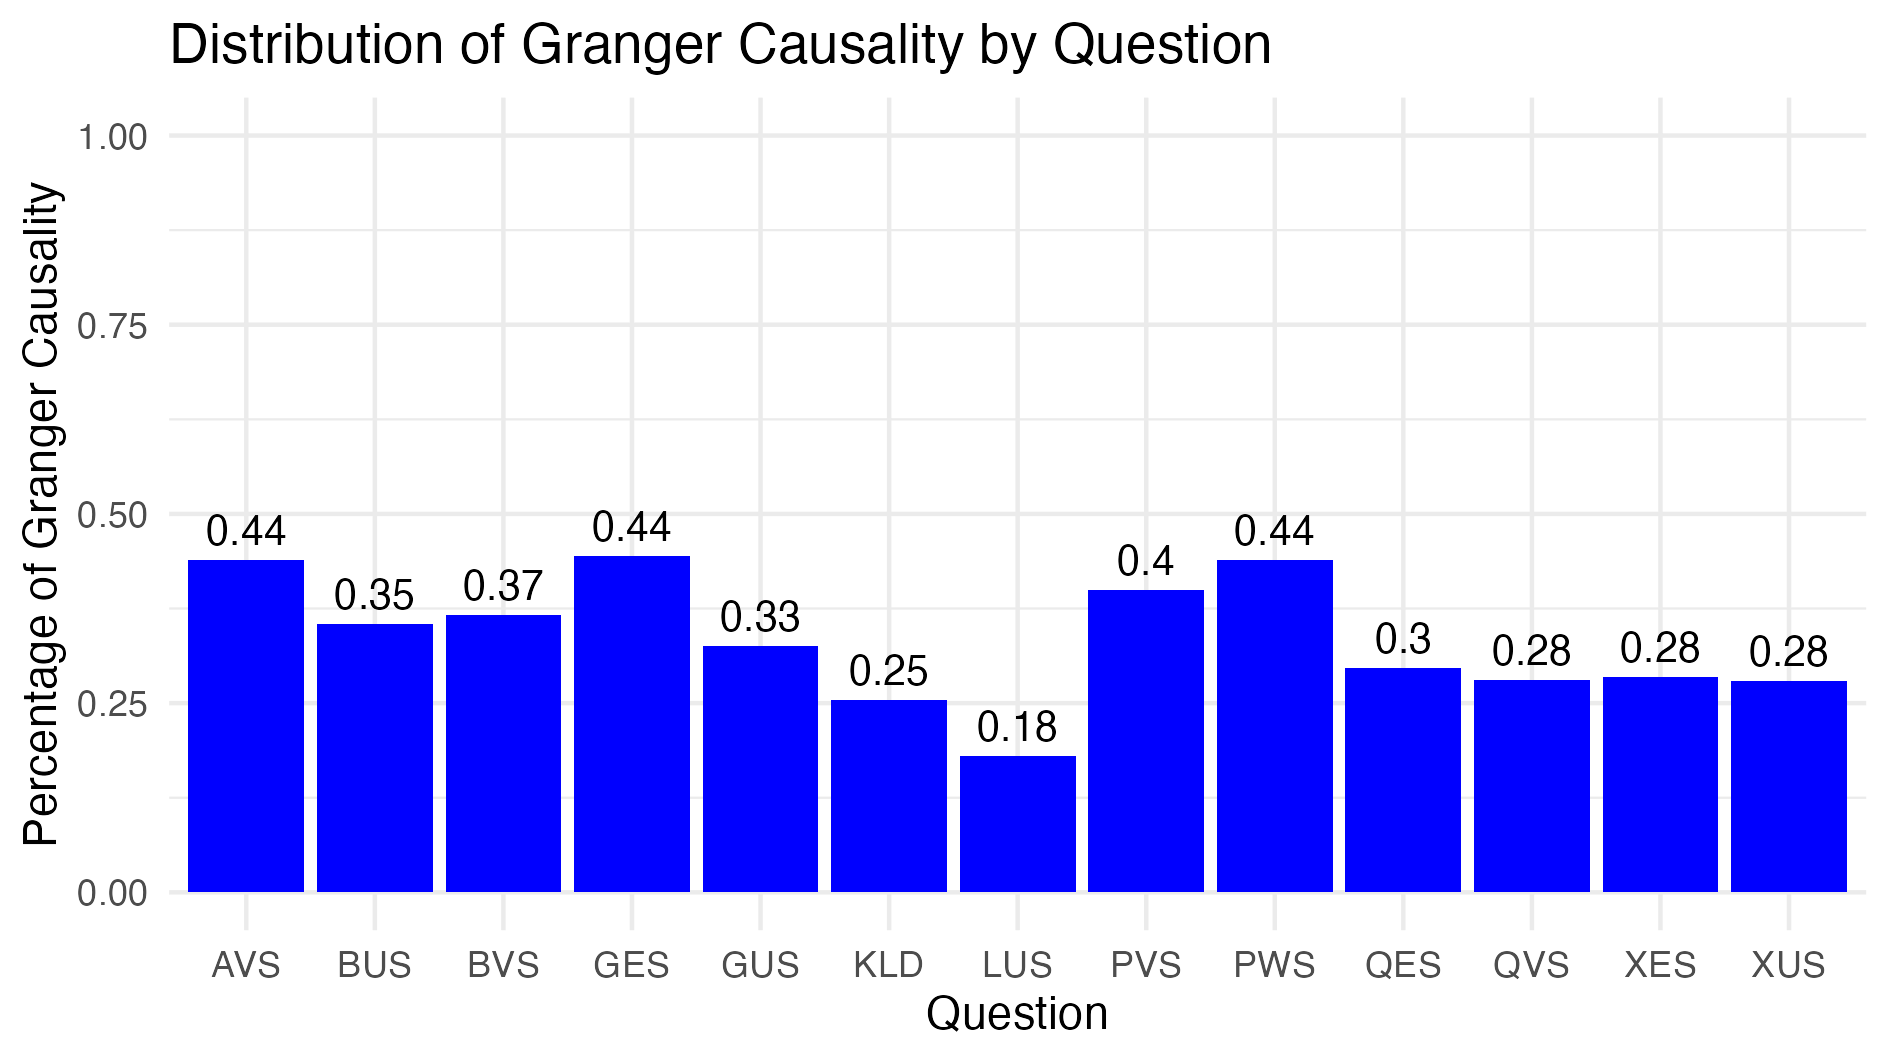
\includegraphics[width=0.9\textwidth]{DanielPlots/distribution_gc_questions_simple.png}
    \caption{Distribution across questions indicating simple Granger causality.}
\end{figure}

The key observations from the data are as follows:

    \begin{itemize}
        \item \textbf{Strongest Predictors}:  AVS, GES, and PWS at 44\% are the strongest predictors with simple Granger Causality, but are far from the 96\% maximum in instantaneous Granger Causality
        \item The predictive power of the KLD survey question for the main index is lost when relying solely on its past values. This suggests that while an industry-specific climate index may serve as a valid proxy for a contemporaneous assessment of the main index, it is insufficient for forecasting its future values.


    \end{itemize}




\textbf{Magnitude of information gain}
\newline
Compared to instantaneous Granger Causality the maximum information gain in terms of adjusted $R^2$ is even lower at 0.0073 (compared to 0.0212)
\begin{figure}[H]
    \centering
    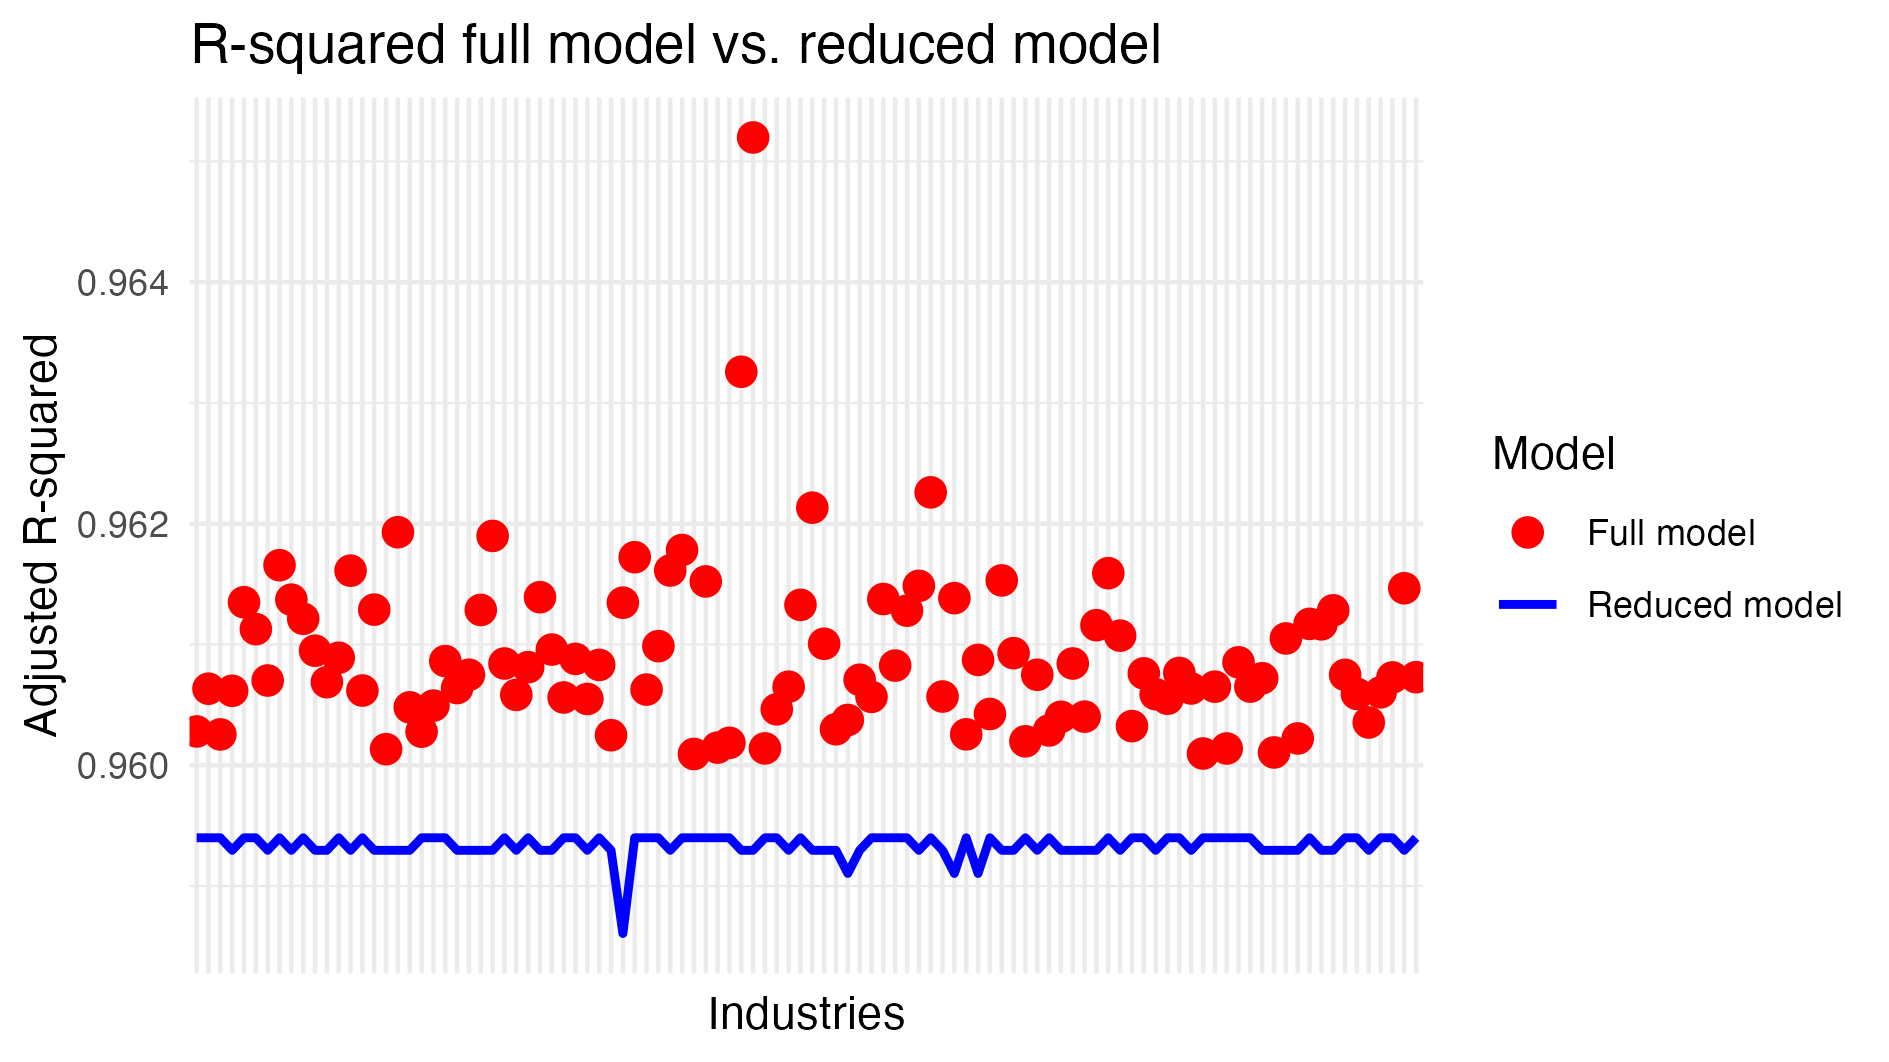
\includegraphics[width=0.8\textwidth]{DanielPlots/adj_r2_plot_simple.png}
    \caption{Adjusted $R^2$ differences (univariate).}
\end{figure}



\renewcommand{\arraystretch}{1.3}
\begin{table}[H]
\small
\centering
\begin{tabularx}{\textwidth}{X c c c}
\toprule
\textbf{Industry} & \textbf{Question} & \textbf{Lag} & \textbf{diff. adj. $R^2$} \\
\midrule
Manufacturing of tools      & business expectations      & 1   & 0.00730      \\
Manufacturing of cutting devices, tools, and locks       & business expectations      & 1   & 0.00714      \\
Manufacturing of forged, pressed, drawn, and stamped parts       & business expectations      & 1   & 0.00701      \\
Manufacturing plastic goods (C2220000)       & business expectations      & 1   & 0.00660      \\
Manufacturing of other plastic goods (C2229000)     & business expectations      & 1   & 0.00657      \\
\bottomrule
\end{tabularx}
\caption{Top 5 industries by difference in adjusted $R^2$ (univariate).}
\end{table}





\subsection{Conclusion for Granger Causality}
Statistical analysis indicates that disaggregated survey data from a vast majority of individual industries, across both 2-digit and 3-digit classification levels, is Granger causal (simple and instantaneous) to the main-index. The robustness of this finding is underscored by the observation that this relationship was absent in only a few of the more than one hundred industries analyzed. However, while these relationships are statistically significant and do possess predictive power for the aggregate index, the marginal information gain from any single industry is negligible and therefore does not meaningfully improve the model's predictive performance. Additionally an implicit requirement for Granger causality is stationarity which is violated in some survey questions and industries as outlined in \ref{stationarity}. Further analysis could examine groups of industries to predict the main index.
\newpage
%--------------------------------------------------------------------------------

%--------------------------------------------------------------------------------
\section{Indicative Subsets}
\label{ch:ind_subsets}
We already established the existence of lead--lag structures between different questions and industry codes. A central goal is therefore to identify industries that allow us to predict the main index reliably. To enhance stability, we focus not on single industries but rather on subsets of industry codes.

The central idea is to identify subsets of industries that allow reliable prediction of the main index. To this end, we construct prediction sets based on lead--lag profiles. Specifically, we distinguish between a \emph{Prediction Set}, which covers leads of one to six months, and an \emph{Early Prediction Set}, which focuses on leads of four to six months. Industry codes are selected using different strategies, including sparse linear models, the scoring model, and clustering approaches. The resulting sets are then evaluated against benchmark models that rely solely on lagged values of the main index.

\subsection{Elastic Net}
The identification of smaller representative subsets can also be formulated as the problem of fitting a sparse regression model. A common way to induce sparsity is to include an $\ell_1$ penalty term in the objective function. In this study we apply the Elastic Net, which combines an $\ell_1$ penalty with an additional $\ell_2$ penalty. The latter helps to stabilize the estimation process in the presence of multicollinearity, while the $\ell_1$ component drives variable selection and promotes sparsity. The Elastic Net objective is given by
\[
\min_{\beta_0,\beta}\;\frac{1}{2N}\sum_{i=1}^n\bigl(y_i-\beta_0-x_i^\top\beta\bigr)^2+\lambda\Bigl((1-\alpha)\lVert\beta\rVert_2^2+\alpha\lVert\beta\rVert_1\Bigr),
\]
where $\lambda$ controls the overall degree of regularization and $\alpha$ determines the balance between the $\ell_1$ and $\ell_2$ components.  

Because the number of observations is relatively small compared to the large set of potential predictors, feature preselection was applied to improve stability and interpretability of the results. In particular, we restricted the predictor set to industry codes at level~2, which provides a manageable yet sufficiently rich representation of sectoral dynamics.

\subsection{Scoring Model}
Two challenges we faced when selecting industry codes for predictions is that 
Simple correlations between industry codes and the main index vary substantially across windows and questions, and rank-based approaches often inflate the size of selected sets when consensus is low. To address this, we develop a scoring model that provides a stable and comparable measure of predictive power across time and survey questions. The goal is to assign each industry code a single score that reflects its predictive relevance and allows for consistent selection of the top-$k$ industries.

The scoring model is designed to capture both the strength and the variability of correlations, while also reflecting structural patterns across questions and windows. Importantly, it provides not only a ranking of industries but also meaningful distances between them.

\vspace{\baselineskip}
For each window $t$, question $q$, and industry $i$, we compute the peak correlation $c_{i,t,q}$. We then define the relative performance
\[
r_{i,t,q}=c_{i,t,q}-\max_j c_{j,t,q},
\]
and aggregate across all windows and questions to obtain
\[
\mathrm{Score}_i=\frac{1}{TQ}\sum_{t,q} r_{i,t,q}^2.
\]
This formulation yields stable scores, where the squared deviations measure the distance of each industry to the pointwise best performer.

As illustrated in Figure~\ref{fig:sm_score_avg_min}, the average and minimum scores for the top-ranked industries are very close to one another, while towards the lower end the scores drop steeply. This pattern indicates that although predictive performance is relatively strong across a wide range of industries, a smaller subset consistently stands out. The scoring model thus provides a principled way to identify predictive sets and complements the other selection approaches.

\begin{figure}[H]
    \centering
    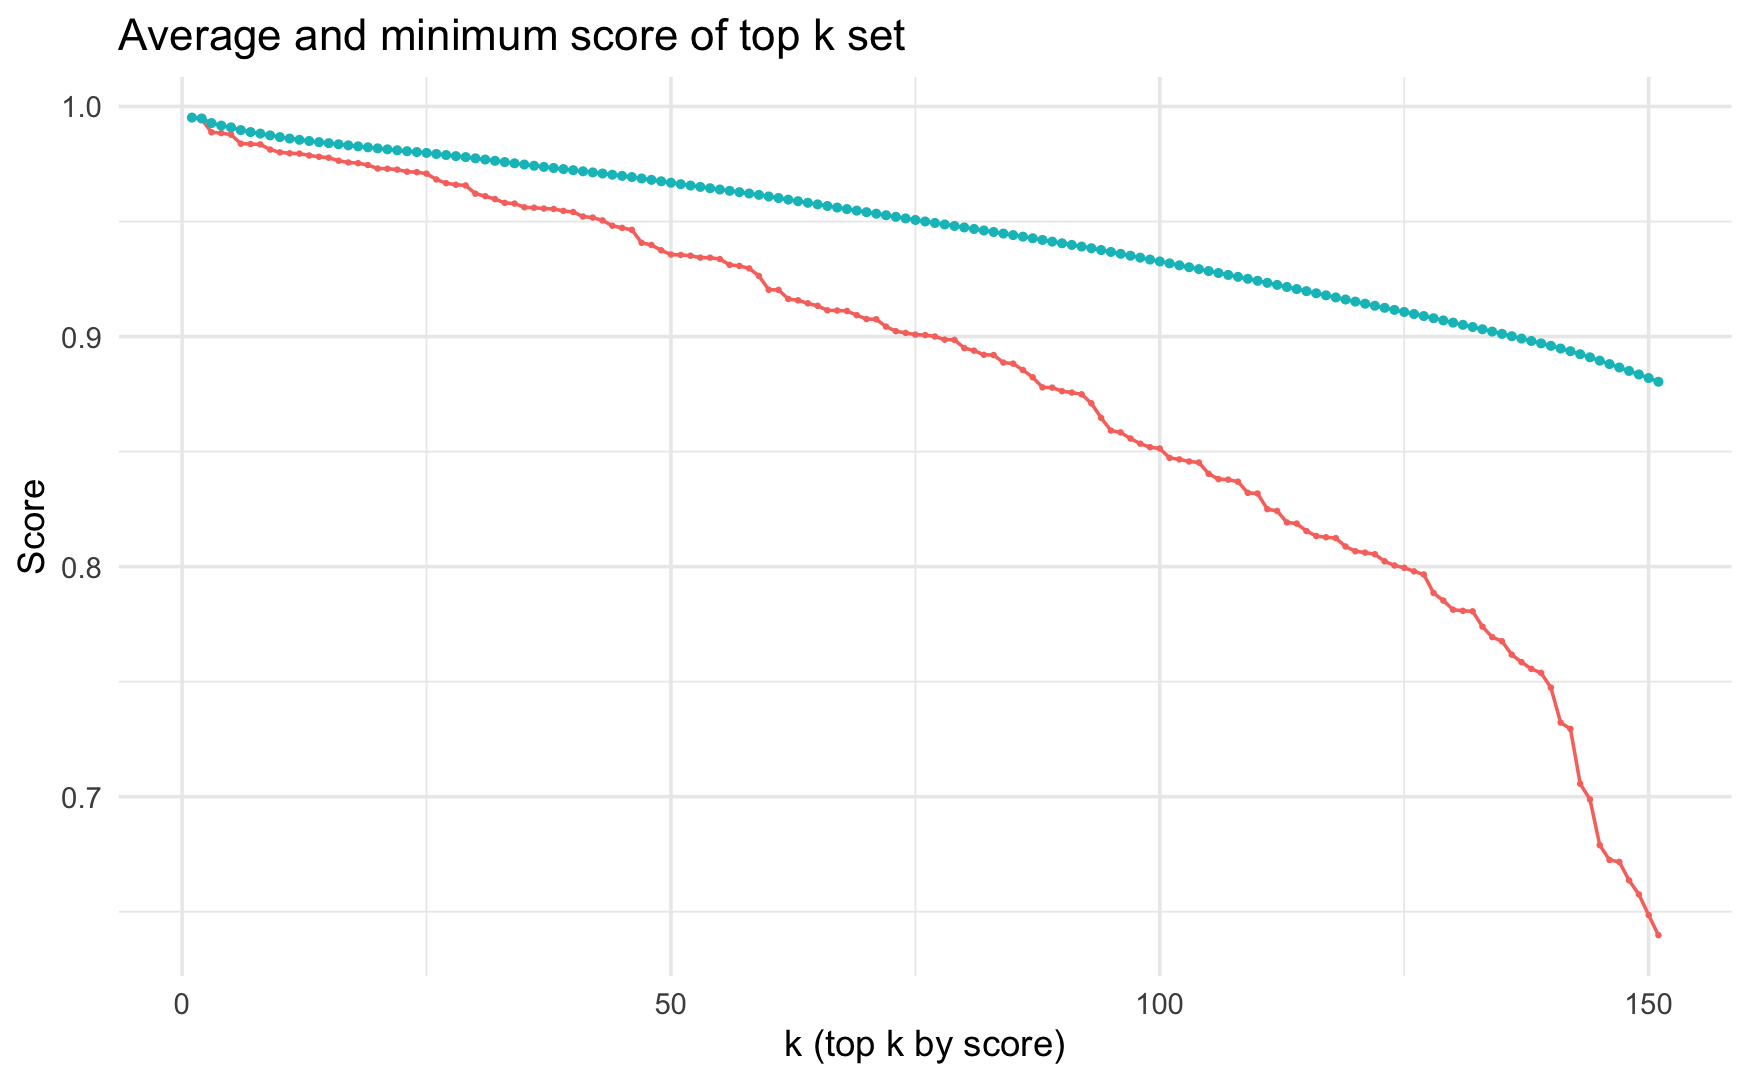
\includegraphics[width=0.8\linewidth]{DominikPlots/sm_score_avg_min.png}
    \caption{Prediction performance (Prediction Set).}
    \label{fig:sm_score_avg_min}
\end{figure}


\subsection{Model Performance}
In the following, we compare the performance of the industry codes selected by the Elastic Net and the Scoring Model. For both approaches, we fit a linear model that includes the selected industry codes together with the lagged main index. Performance is evaluated in terms of mean squared error (MSE), root mean squared error (RMSE), and the coefficient of determination ($R^2$).

\subsubsection{Prediction Set}
For the scoring model we selected the five highest-scoring industry codes at level~2. The selected industries are listed in Table~\ref{tab:sm_sectors}.

\begin{table}[H]
    \centering
    \caption{Industry codes selected by the Scoring Model}
    \label{tab:sm_sectors}
    \small
    \begin{tabularx}{0.9\linewidth}{lX}
        \toprule
        Code & Name \\
        \midrule
        C1620000 & Manufacture of other products of wood; manufacture of articles of cork, straw and plaiting materials \\
        C1720000 & Manufacture of articles of paper and paperboard \\
        C2220000 & Manufacture of plastic products \\
        C2440000 & Manufacture of basic precious and other non-ferrous metals \\
        C2890000 & Manufacture of other special-purpose machinery \\
        \bottomrule
    \end{tabularx}
\end{table}

These industries are predominantly associated with packaging materials, intermediate goods, and investment goods such as machinery. From an economic perspective, this selection is plausible: packaging and input materials are required early in the production process, and machinery is ordered in anticipation of future demand. Consequently, these sectors are likely to lead the overall economic development, with orders placed in advance during expansions and cancelled early in recessions.

The Elastic Net procedure selected a somewhat different set of industries, shown in Table~\ref{tab:en_sectors}. While the codes differ from those identified by the scoring model, the economic interpretation is similar: these industries also represent upstream or investment-oriented activities that tend to react early to changes in the business cycle.

\begin{table}[htbp]
    \centering
    \caption{Industry codes selected by the Elastic Net}
    \label{tab:en_sectors}
    \small
    \begin{tabularx}{0.9\linewidth}{lX}
        \toprule
        Code & Name \\
        \midrule
        C2550000 & Forging, pressing, stamping and roll-forming of metal; powder metallurgy \\
        C2560000 & Treatment and coating of metals; machining \\
        C2840000 & Manufacture of machine tools \\
        C2920000 & Manufacture of bodies (coachwork) for motor vehicles; manufacture of trailers and semitrailers \\
        \bottomrule
    \end{tabularx}
\end{table}

\vspace{\baselineskip}
Because the models differ in the number of predictors, we evaluate performance using $R^2$ rather than adjusted $R^2$. The results are reported in Table~\ref{tab:ps_results}. Both selection methods achieve a higher fit than the benchmark model based solely on the lagged main index. The scoring model performs slightly better than the Elastic Net, although the differences are modest. This outcome is in line with expectations: given its smaller set of selected features, the Elastic Net is likely to perform somewhat worse than the scoring model but still slightly better than the lagged benchmark.

\begin{table}[H]
    \centering
    \caption{Prediction performance (Prediction Set)}
    \label{tab:ps_results}
    \small
    \begin{tabular}{lccc}
        \toprule
         & \textbf{MSE} & \textbf{RMSE} & \textbf{$R^2$}\\
        \midrule
        Scoring Model     & 9.48 & 3.08 & 0.97 \\
        Elastic Net       & 9.99 & 3.16 & 0.96 \\
        Lagged Main Index & 11.00 & 3.32 & 0.96 \\
        \bottomrule
    \end{tabular}
\end{table}

Figure~\ref{fig:ps_pred_performance} plots the model predictions against the observed main index. As expected, all models track the actual development closely. This is not surprising, since a lead of one month is economically short and provides relatively limited scope for divergence.

\begin{figure}[H]
    \centering
    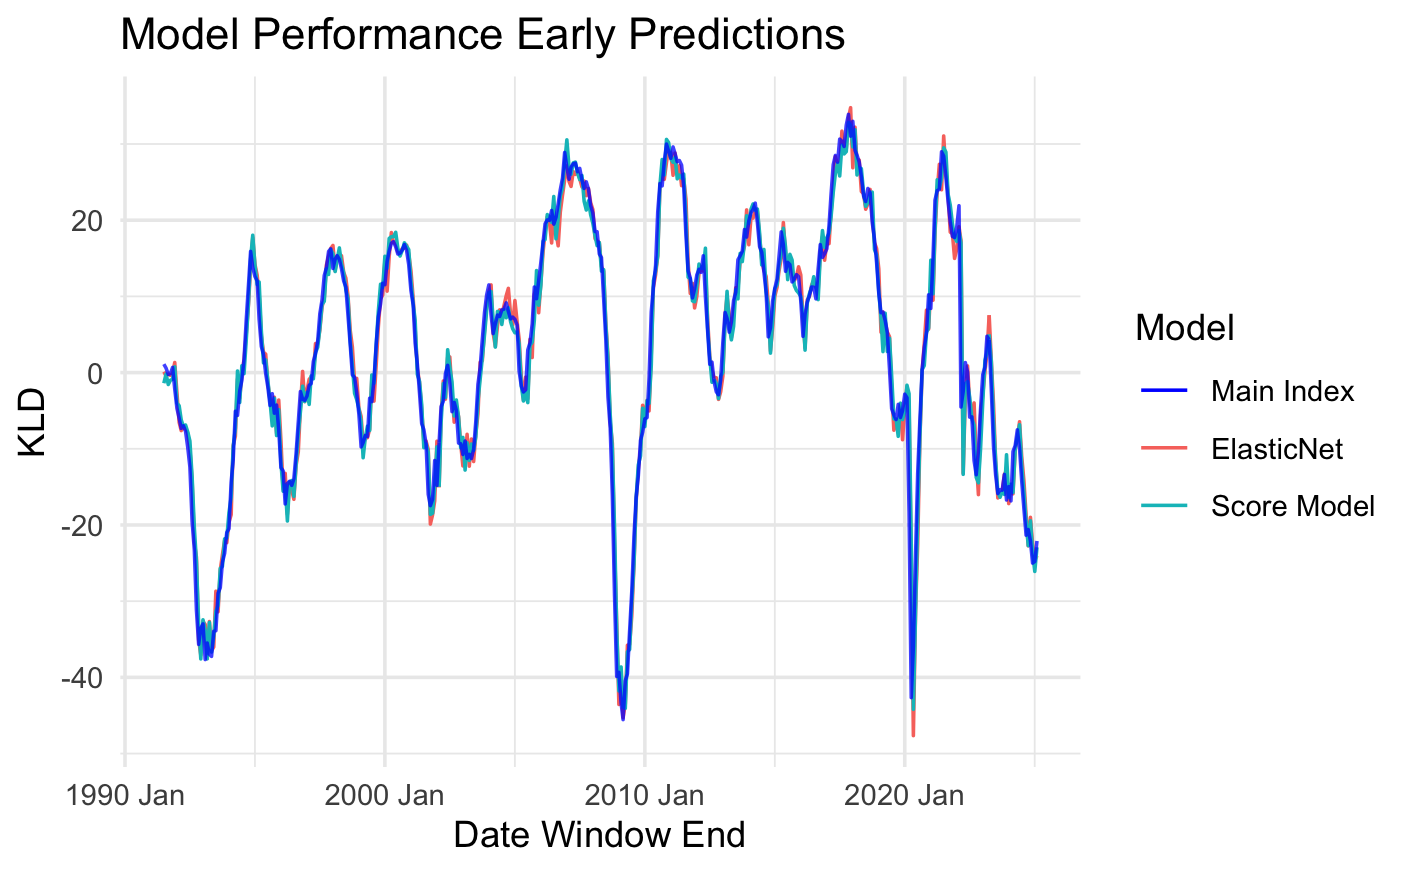
\includegraphics[width=0.8\linewidth]{DominikPlots/ps_pred_performance.png}
    \caption{Prediction performance of different models (Prediction Set).}
    \label{fig:ps_pred_performance}
\end{figure}


\subsubsection{Early Prediction Set}
For the early prediction set we restricted the lead to four to six months, thereby focusing on industries that provide signals further in advance. The selected industries are shown in Tables~\ref{tab:sm_sectors_early} and \ref{tab:en_sectors_early}. While the sets partly differ from those in the general prediction set, there is notable overlap in the types of sectors identified, underlining the same economic reasoning: industries producing upstream inputs or investment goods tend to react early to changes in demand expectations.

\begin{table}[htbp]
    \centering
    \caption{Industry codes selected by the Scoring Model (Early Prediction Set)}
    \label{tab:sm_sectors_early}
    \small
    \begin{tabularx}{0.9\linewidth}{lX}
        \toprule
        Code & Name \\
        \midrule
        C1610000 & Sawmilling and planing of wood \\
        C1710000 & Manufacture of pulp, paper and paperboard \\
        C1720000 & Manufacture of articles of paper and paperboard \\
        C2220000 & Manufacture of plastic products \\
        C2440000 & Manufacture of basic precious and other non-ferrous metals \\
        \bottomrule
    \end{tabularx}
\end{table}

\begin{table}[H]
    \centering
    \caption{Industry codes selected by the Elastic Net (Early Prediction Set)}
    \label{tab:en_sectors_early}
    \small
    \begin{tabularx}{0.9\linewidth}{lX}
        \toprule
        Code & Name \\
        \midrule
        C1610000 & Sawmilling and planing of wood \\
        C2550000 & Forging, pressing, stamping and roll-forming of metal; powder metallurgy \\
        C2560000 & Treatment and coating of metals; machining \\
        C2920000 & Manufacture of bodies (coachwork) for motor vehicles; manufacture of trailers and semitrailers \\
        \bottomrule
    \end{tabularx}
\end{table}

As in the general prediction set, we evaluate the performance of the scoring model, the Elastic Net, and the benchmark model based on lagged values of the main index. The results are summarized in Table~\ref{tab:early_results}. Both selection methods outperform the benchmark, with the scoring model again achieving slightly better predictive accuracy than the Elastic Net.

\begin{table}[H]
    \centering
    \caption{Prediction performance (Early Prediction Set)}
    \label{tab:early_results}
    \small
    \begin{tabular}{lccc}
        \toprule
         & \textbf{MSE} & \textbf{RMSE} & \textbf{$R^2$} \\
        \midrule
        Scoring Model     & 63.00 & 7.94 & 0.77 \\
        Elastic Net       & 66.00 & 8.12 & 0.76 \\
        Lagged Main Index & 79.40 & 8.91 & 0.71 \\
        \bottomrule
    \end{tabular}
\end{table}

Figure~\ref{fig:ps_earlypred_performance} plots the model predictions against the observed main index. Compared to the one-month lead predictions, the increased horizon naturally leads to a lower overall fit. Nonetheless, both the scoring model and the Elastic Net improve substantially over the lagged benchmark, confirming the usefulness of early-predictive industry codes.

\begin{figure}[H]
    \centering
    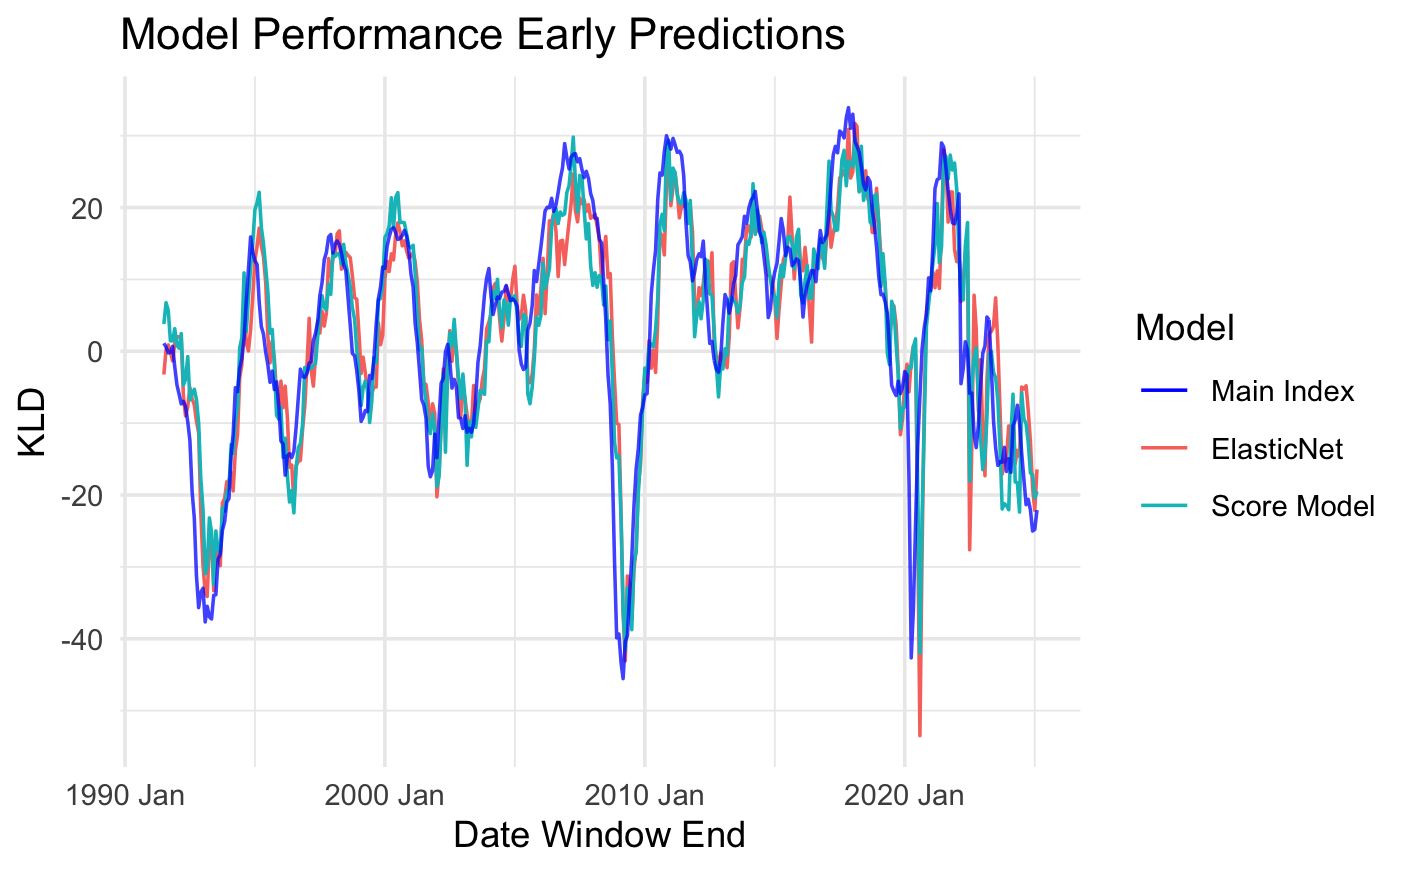
\includegraphics[width=0.8\linewidth]{DominikPlots/ps_earlypred_performance.png}
    \caption{Prediction performance of different models (Early Prediction Set).}
    \label{fig:ps_earlypred_performance}
\end{figure}


\subsubsection{Performance Comparison and Interpretation}

The comparison of cross-correlation profiles highlights important differences between the two selection approaches. As shown in Figures~\ref{fig:comparison_pred_profiles} and \ref{fig:comparison_earlypred_profiles}, the Sparse LM (Elastic Net) identifies industry codes with stronger lead properties, but at the cost of weaker overall correlations. By contrast, the scoring model yields a more robust correlation structure, although peak correlations tend to occur at shorter leads. This reflects the design of the scoring model: by penalizing outliers more heavily, it favors industry codes that exhibit consistently strong correlations across questions and windows, thereby providing a more ``general'' solution.

\begin{figure}[H]
    \centering
    \begin{subfigure}[t]{0.48\linewidth}
        \centering
        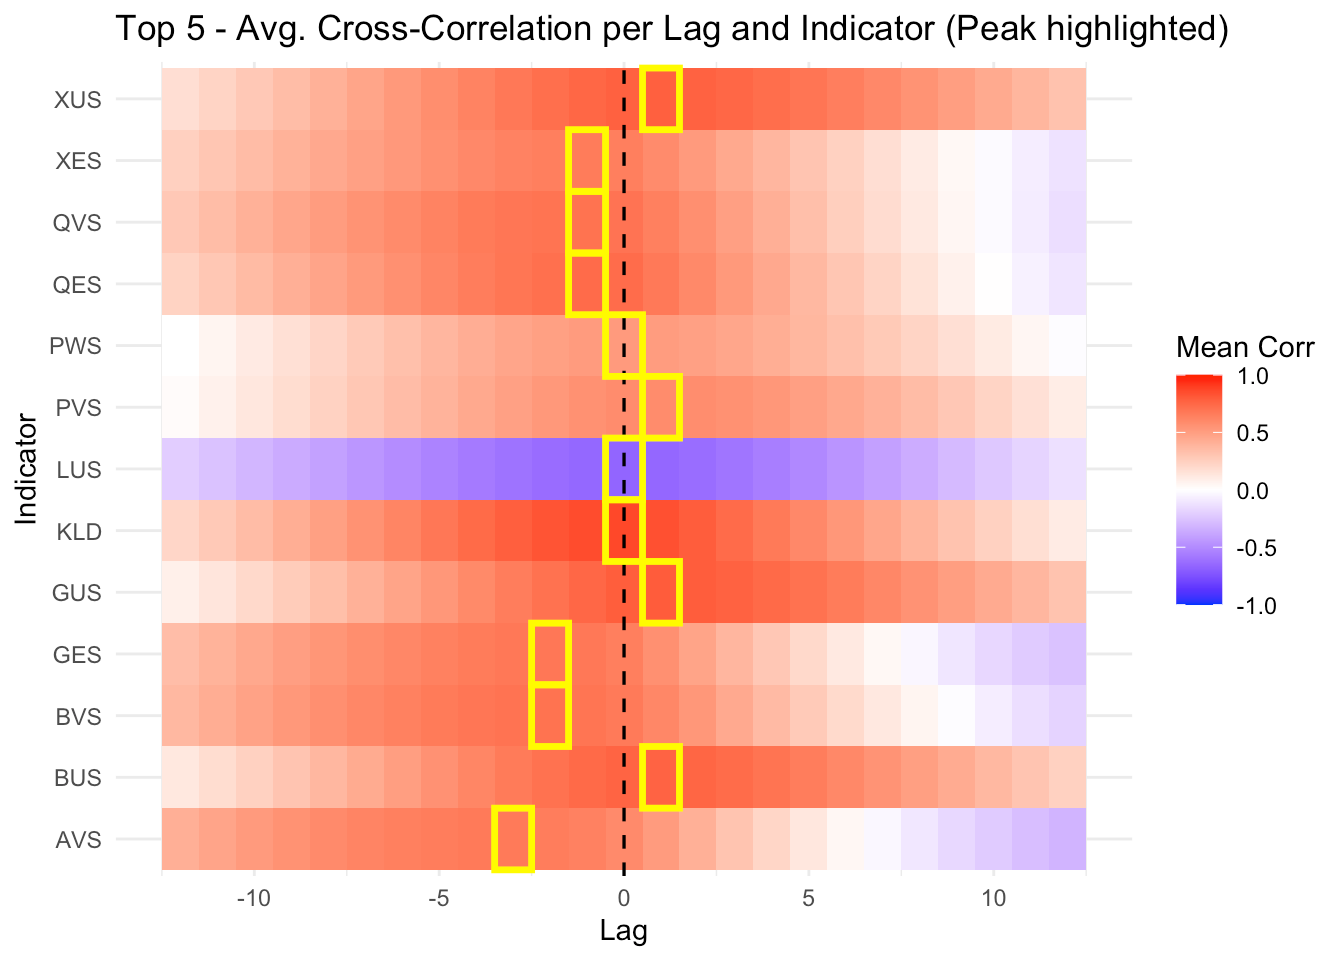
\includegraphics[width=\linewidth]{DominikPlots/ps_score_pred_ccf.png}
        \caption{Prediction Set (Scoring Model).}
        \label{fig:median_score_pred_ps}
    \end{subfigure}%
    \hfill
    \begin{subfigure}[t]{0.48\linewidth}
        \centering
        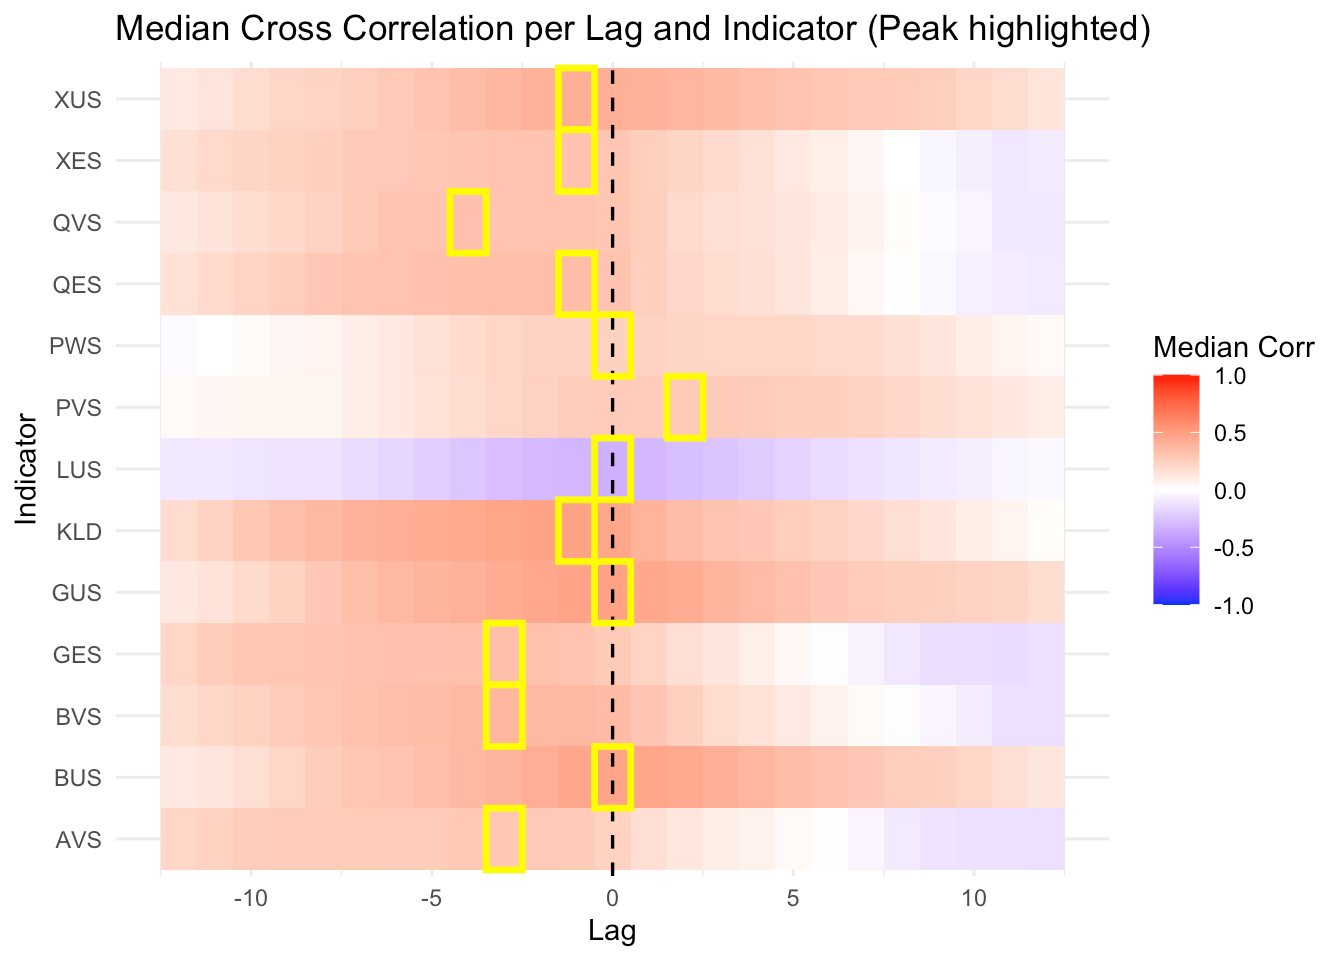
\includegraphics[width=\linewidth]{DominikPlots/ps_lm_pred_ccf.png}
        \caption{Prediction Set (Sparse LM).}
        \label{fig:median_lm_pred_ps}
    \end{subfigure}
    \caption{Comparison of median cross-correlation profiles across industries for the Prediction Set. Yellow boxes indicate peak lags; vertical dashed line marks zero.}
    \label{fig:comparison_pred_profiles}
\end{figure}

\begin{figure}[H]
    \centering
    \begin{subfigure}[t]{0.48\linewidth}
        \centering
        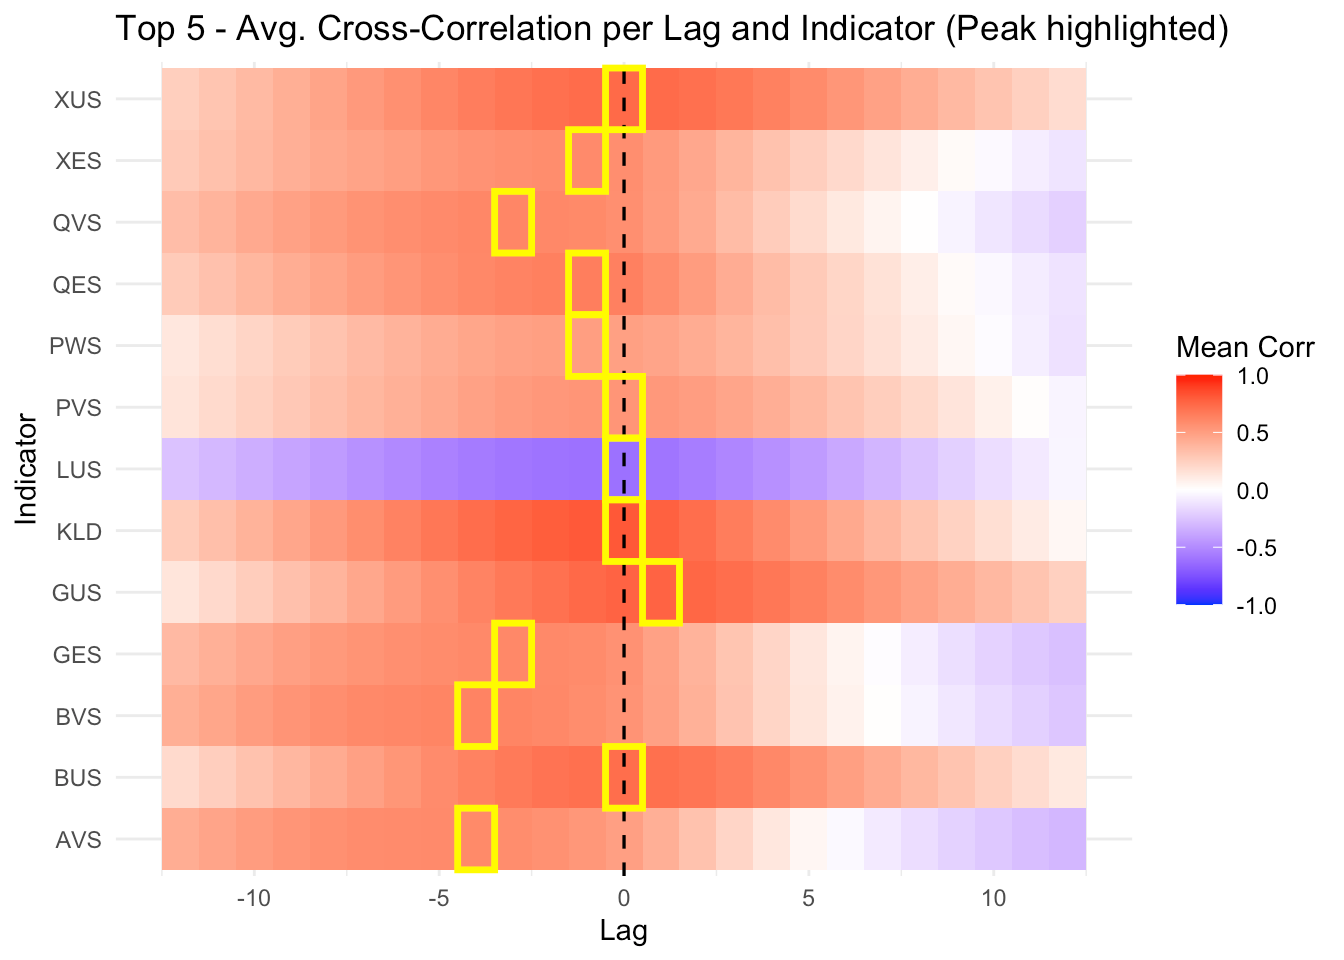
\includegraphics[width=\linewidth]{DominikPlots/ps_score_earlypred_ccf.png}
        \caption{Early Prediction Set (Scoring Model).}
        \label{fig:median_score_pred_early}
    \end{subfigure}%
    \hfill
    \begin{subfigure}[t]{0.48\linewidth}
        \centering
        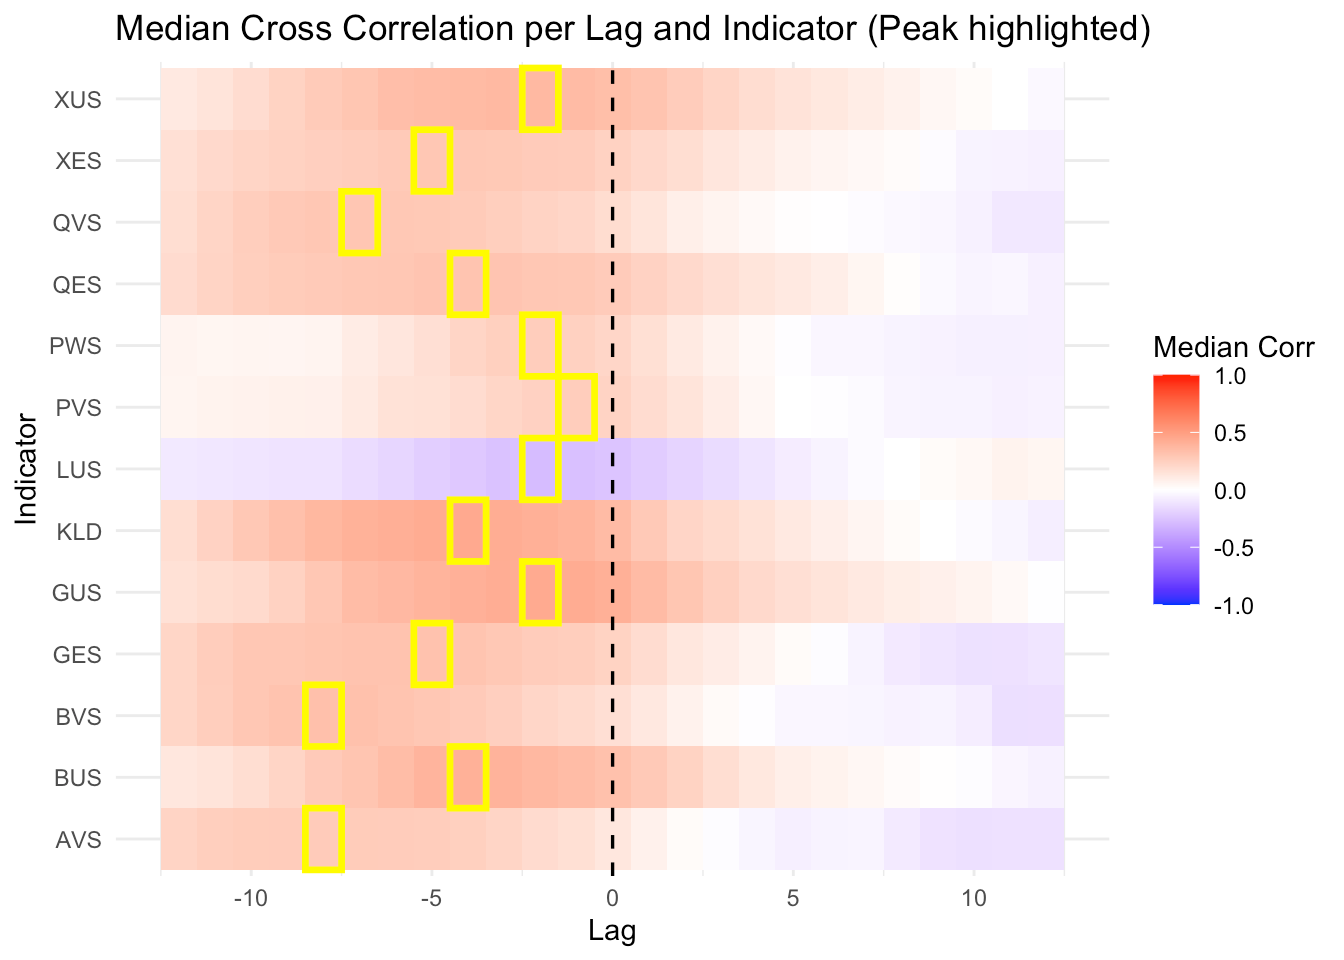
\includegraphics[width=\linewidth]{DominikPlots/ps_lm_earlypred_ccf.png}
        \caption{Early Prediction Set (Sparse LM).}
        \label{fig:median_lm_pred_early}
    \end{subfigure}
    \caption{Comparison of median cross-correlation profiles across industries for the Early Prediction Set (lead 4--6 months).}
    \label{fig:comparison_earlypred_profiles}
\end{figure}

Lagging questions such as BUS and GUS show relatively low lags of peak correlation, illustrating how the two strategies emphasize distinct aspects of predictive performance. The scoring model captures industries with dynamics broadly similar to the main index, which results in highly correlated predictor sets. The $\ell_1$ component underlying the Sparse LM encourages selection of more distinct predictors by retaining one representative from groups of highly correlated industries and discarding the rest; a small $\ell_2$ component (Elastic Net) is included to stabilize estimation under multicollinearity \citep[cf.][]{ZouHastie2005}. This methodological difference helps explain why the selected subsets diverge and why the average correlation strength varies between methods.

To assess robustness, we additionally compare both methods to 500 random subsets of five level-2 industry codes. Figures~\ref{fig:comparison_random_sets}a and~\ref{fig:comparison_random_sets}b display the distribution of $R^2$ across these random subsets. As expected, nearly all subsets outperform the benchmark based solely on lagged main-index values. The scoring model consistently ranks among the stronger subsets, supporting its usefulness as a versatile selection method for predictive modeling.

\begin{figure}[H]
    \centering
    \begin{subfigure}[t]{0.48\linewidth}
        \centering
        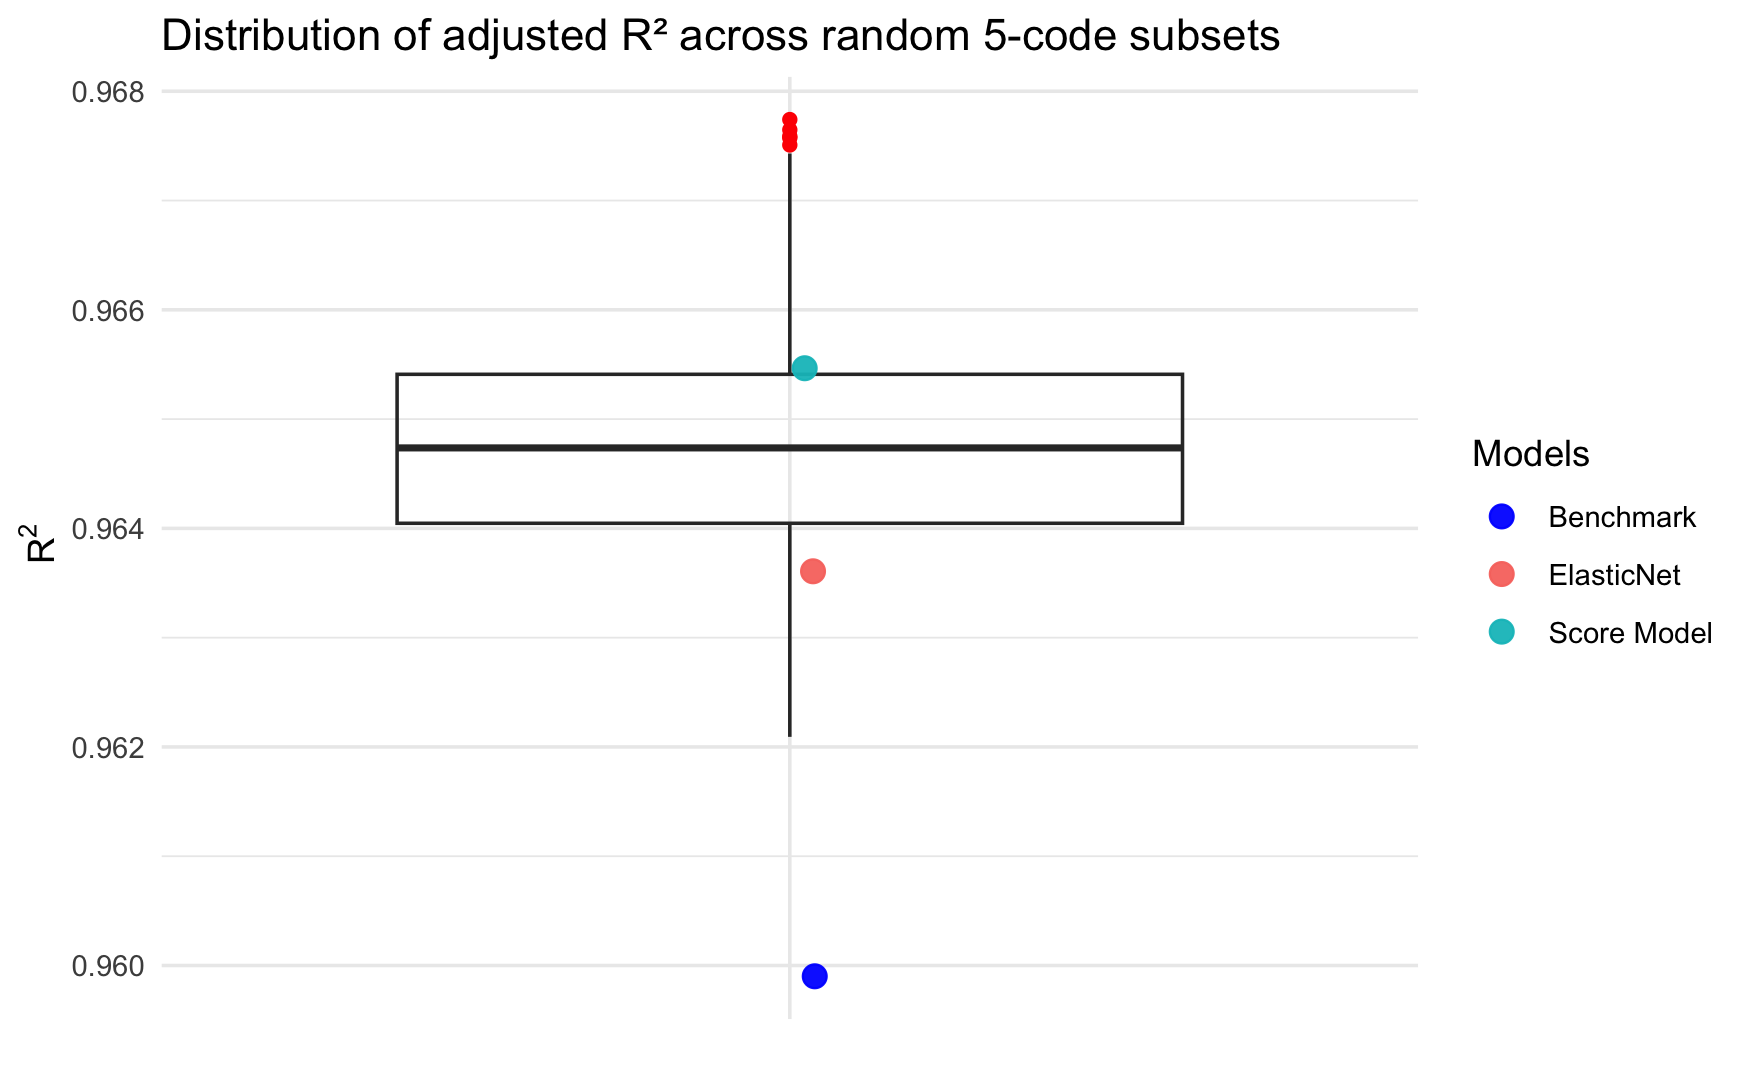
\includegraphics[width=\linewidth]{DominikPlots/ps_pred_random.png}
        \caption{Prediction Set.}
        \label{fig:random_pred}
    \end{subfigure}%
    \hfill
    \begin{subfigure}[t]{0.48\linewidth}
        \centering
        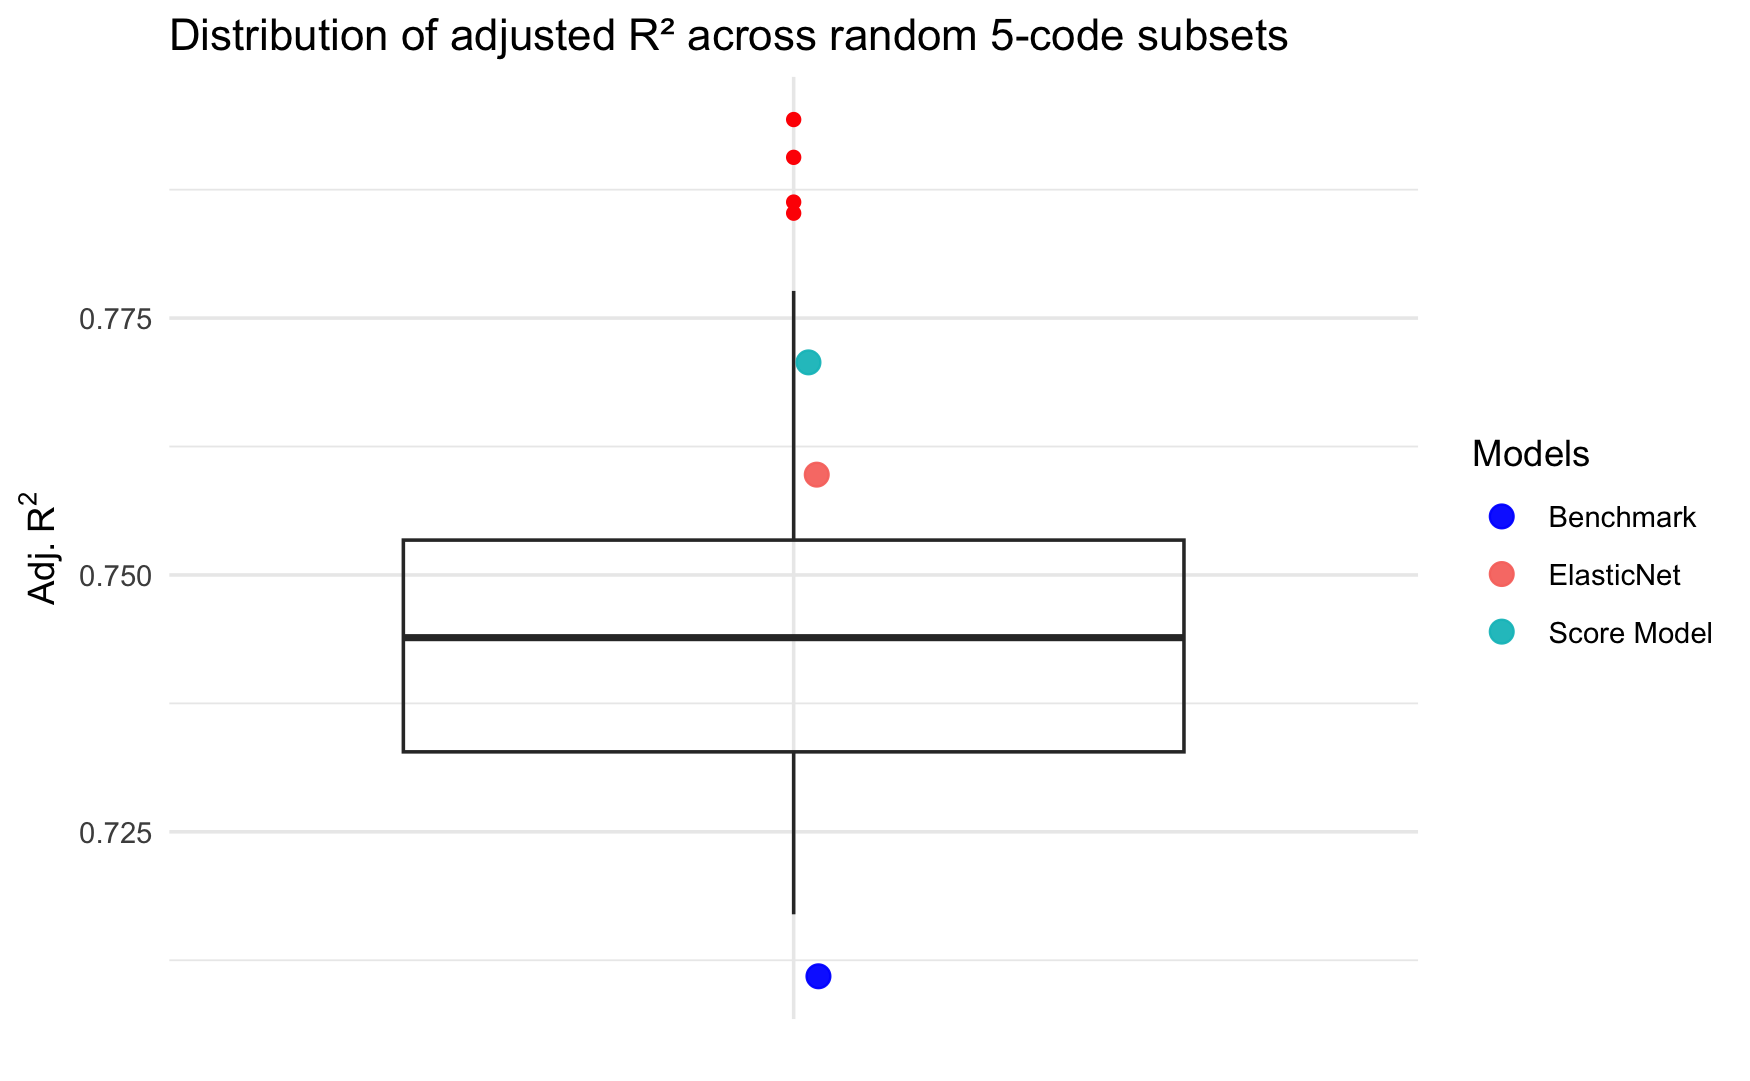
\includegraphics[width=\linewidth]{DominikPlots/ps_earlypred_random.png}
        \caption{Early Prediction Set.}
        \label{fig:random_earlypred}
    \end{subfigure}
    \caption{Distribution of $R^2$ across 500 random 5-code subsets, with benchmark (lagged main index), Elastic Net, and Scoring Model overlaid.}
    \label{fig:comparison_random_sets}
\end{figure}

\vspace{\baselineskip}
At the top end of the distribution, performance is dominated by a small number of outlier subsets. Tables~\ref{tab:random_subsets} and \ref{tab:random_subsets2} list the three best-performing random subsets for the Prediction Set and the Early Prediction Set, respectively. Notably, each table contains twelve distinct industry codes across only three subsets (3$\times$5), indicating that strong predictive performance is not confined to a unique combination of industries. Rather, what matters are shared economic characteristics: upstream inputs, packaging/intermediate goods, and investment-related sectors tend to provide early signals of cyclical turning points.

\begin{table}[H]
    \centering
    \caption{Top 3 random subsets (Prediction Set)}
    \label{tab:random_subsets}
    \small
    \begin{tabularx}{0.9\linewidth}{Xcc}
        \toprule
        \textbf{Industry Codes} & \textbf{$R^2$} & \textbf{RMSE} \\
        \midrule
        C1720000, C2210000, C2590000, C2450000, C2390000 & 0.968 & 2.98 \\
        C1610000, C2740000, C3250000, C2710000, C2450000 & 0.968 & 2.98 \\
        C2570000, C2440000, C1720000, C2310000, C2710000 & 0.968 & 2.98 \\
        \bottomrule
    \end{tabularx}
\end{table}

\begin{table}[H]
    \centering
    \caption{Top 3 random subsets (Early Prediction Set)}
    \label{tab:random_subsets2}
    \small
    \begin{tabularx}{0.9\linewidth}{Xcc}
        \toprule
        \textbf{Industry Codes} & \textbf{$R^2$} & \textbf{RMSE} \\
        \midrule
        C1610000, C2920000, C2910000, C2930000, C1060000 & 0.794 & 7.52 \\
        C2610000, C1610000, C2340000, C1710000, C2310000 & 0.791 & 7.58 \\
        C2550000, C2340000, C3250000, C1610000, C2040000 & 0.786 & 7.66 \\
        \bottomrule
    \end{tabularx}
\end{table}


Multiple paths exist to construct effective predictive sets. The scoring model offers stability and interpretability by selecting industries with consistently strong correlations to the main index across questions and windows. The Elastic Net (Sparse LM) promotes diversity by emphasizing distinct predictors and stabilizes estimation via an additional $\ell_2$ component. Random subsets demonstrate that predictive skill is widely distributed across industries, yet especially pronounced among upstream and investment-oriented sectors.

\newpage
\subsection{Clustering based on CCF}
So far, we have mostly considered all questions within each industry. To find potentially leading groups, which can contain different questions of different industries, we took on a clustering approach based their relationship with the main index. We computed the CCF of all individual questions of all level 2 aggregates and then performed Ward's method to cluster them \citep{ward1963hierarchical}. In a nutshell, Ward's method starts with each component as its own cluster and iteratively merges clusters in a way that minimizes the overall within-cluster variance.

\subsubsection{Comparing cluster groups}
A challenge lied in finding a good measure to compare the resulting groups and rank out potentially interesting ones. Simply ranking clusters by correlation strength does not distinguish between leading and lagging behavior. To address this, we adopted a similar strategy as in the previous methods: we fitted a linear model predicting the main index $y$ using its own lagged values along with the lagged values of a cluster average $x$ up to lag $k$:
\[
y_t \sim y_{t-1} + y_{t-2} + ... + y_{t-k} + x_{t-1} + x_{t-2} + ... + x_{t-k} 
\]
Again, we used one setting with all lagged values up to 6 months behind and another early setting, where we only considered lags 4 to 6. Table~\ref{tab:clusterMSE} shows the top 5 clusters according to the MSE of the above model for both settings. 
\begin{table}[H]
\centering
\small
\begin{subtable}{0.48\textwidth}
\centering
\begin{tabular}{c c c c c}
\toprule
Cluster & $n$ & MSE & RMSE& Adj. $R^{2}$ \\
\midrule
2  & 9 & 10.27 & 3.21 & 0.9615 \\
10 & 9 & 10.31 & 3.21 & 0.9613 \\
16 & 7 & 10.32 & 3.21 & 0.9613 \\
63 & 8 & 10.37 & 3.22 & 0.9611 \\
62 & 5 & 10.41 & 3.23 & 0.9609 \\
\midrule
Lagged Main & 1 & 11.00 & 3.32 & 0.959 \\
\bottomrule
\end{tabular}
\caption{Considering lags 1 to 6.}
\end{subtable}\hfill
\begin{subtable}{0.48\textwidth}
\centering
\begin{tabular}{c c c c c}
\toprule
Cluster & $n$ & MSE & RMSE & Adj. $R^{2}$ \\
\midrule
63 & 8  & 65.39 & 8.09 & 0.758 \\
48 & 4  & 66.18 & 8.14 & 0.755 \\
1  & 8  & 67.46 & 8.21 & 0.751 \\
3  & 12 & 67.72 & 8.23 & 0.750 \\
5  & 10 & 69.97 & 8.36 & 0.741 \\
\midrule
Lagged Main  & 1 & 79.4 & 8.91 & 0.70\\
\bottomrule
\end{tabular}
\caption{Considering lags 4 to 6}
\end{subtable}
\caption{Top 5 clusters based on MSE}
\label{tab:clusterMSE}
\end{table}

The predictive performance of the above model alone is not necessarily a sufficient indicator to find a meaningfully leading group. Lagged values of a cluster average could add relevant information to the lagged values of the main index, resulting in a low MSE, while still not leading the main index. A visual examination of the CCFs of the cluster can help in further determining leading clusters. Fig.~\ref{fig:cluster_ccf} shows the CCFs of the clusters from table~\ref{tab:clusterMSE}. As expected, more of the top 5 clusters of the early prediction setting seem to be  leading, compared to the other setting. 

\begin{figure}[H]
\centering
\begin{subfigure}{0.48\textwidth}
  \centering
  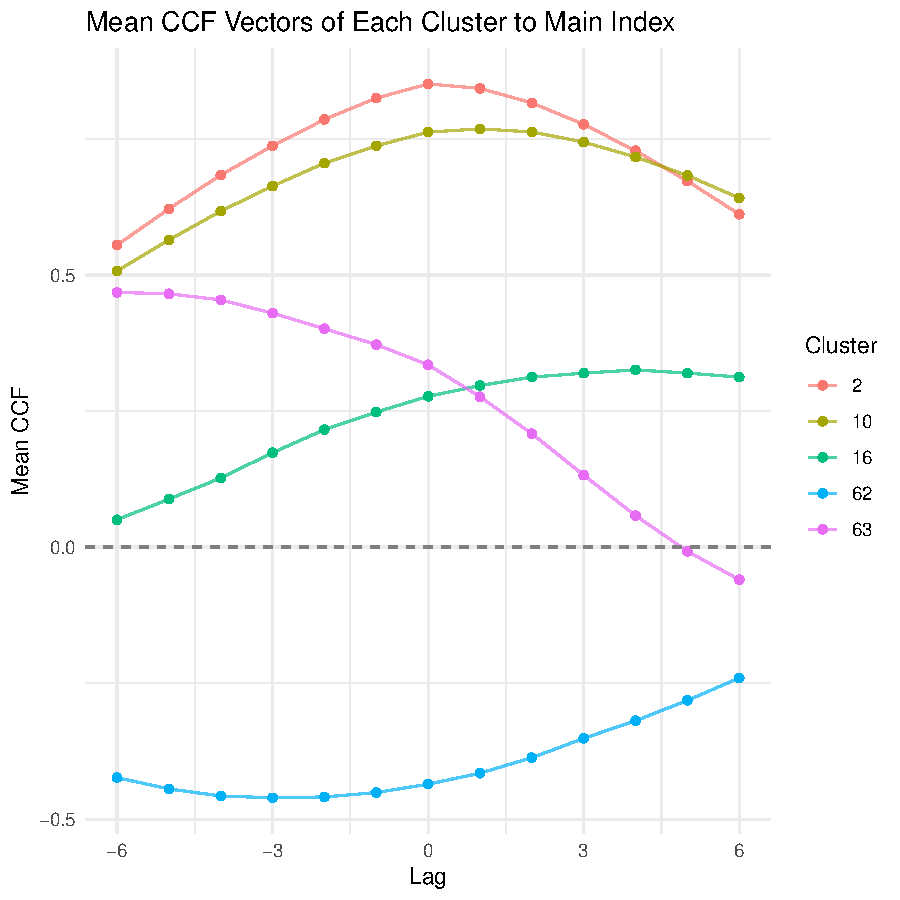
\includegraphics[width=\linewidth]{JakobPlots/ccfs_cluster_plot_1_6.pdf}
  \caption{Top 5 clusters.}
\end{subfigure}\hfill
\begin{subfigure}{0.48\textwidth}
  \centering
  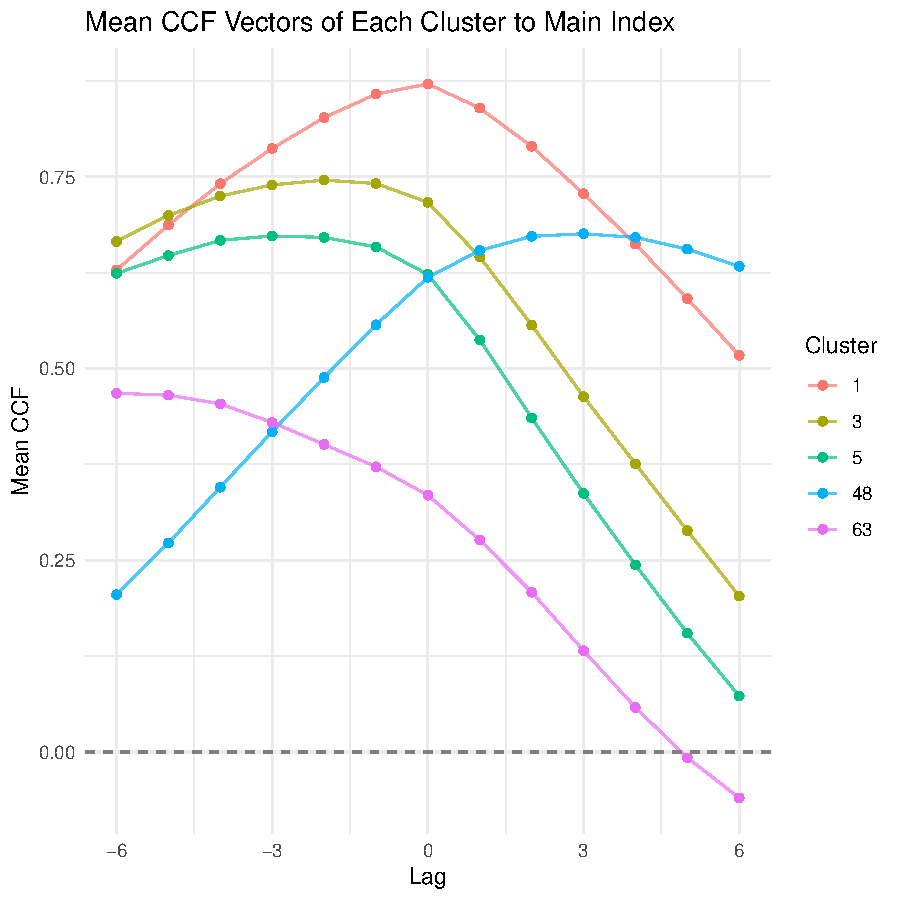
\includegraphics[width=\linewidth]{JakobPlots/ccfs_cluster_plot_4_6.pdf}
  \caption{Top 5 early-predictor clusters.}
\end{subfigure}
\caption{Mean CCFs of the top 5 cluster averages.}
\label{fig:cluster_ccf}
\end{figure}

\subsubsection{Exemplary Cluster}
Although most clusters are difficult to interpret, cluster 3 from the top 5 provides an illustrative example of a potentially meaningful grouping. As shown in Fig.~\ref{fig:cluster3}, the series in this cluster tend to lead the main index, while Table~\ref{tab:cluster3_components} details its constituent components. Its dominated by questions which compare the current situation to the previous month and many of the industries deal with intermediate components or capital goods.

\begin{figure}[H]
    \centering
    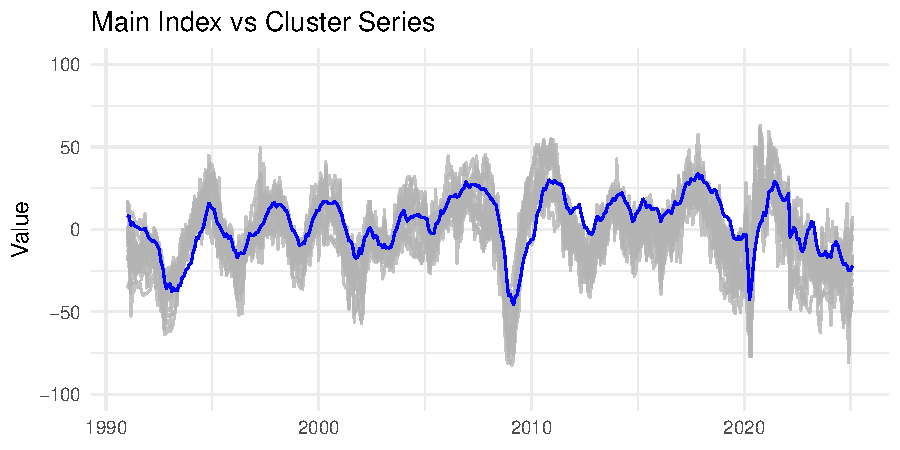
\includegraphics[width=0.8\linewidth]{JakobPlots/3main_plot.pdf}
    \caption{Main index (blue) vs individual series in cluster 3.}
    \label{fig:cluster3}
\end{figure}

\begin{table}[H]
\centering
\footnotesize
\begin{tabular}{ll}
\toprule
\textbf{Industry Title} & \textbf{Question Title} \\
\midrule
Manufacture of plastic products & Business situation expectations \\
Manufacture of plastic products & Order backlog compared to previous month \\
Manufacture of plastic products & Production compared to previous month \\
Manufacture of forged, pressed, drawn, and stamped parts & Order backlog compared to previous month \\
Manufacture of forged, pressed, drawn, and stamped parts & Production compared to previous month \\
Manufacture of forged, pressed, drawn, and stamped parts & Production plans \\
Manufacture of cutlery, tools, and locks & Business situation expectations \\
Manufacture of cutlery, tools, and locks & Demand compared to previous month \\
Manufacture of electric motors, generators, transformers, etc. & Demand compared to previous month \\
Manufacture of non-industry-specific machinery & Demand compared to previous month \\
Manufacture of machine tools & Business situation expectations \\
Paper, cardboard, and paperboard processing & Order backlog compared to previous month \\
\bottomrule
\end{tabular}
\caption{Individual series present in cluster 3.}
\label{tab:cluster3_components}
\end{table}
\newpage
%--------------------------------------------------------------------------------


%--------------------------------------------------------------------------------
\section{Turning Point Indication}
\label{ch:turning_point}
In this final section, we are gonna take a look at whether we can indicate not the main index itself, but rather its turning points. There are several different definitions of economic turning points, and no single standard exists for Germany. We apply the Bry–Boschan algorithm \citep{boschan1971programmed}, as implemented in the R package BCDating \citep{BCDating}, to identify the troughs and peaks of the main index, which serve as the groundtruth. The algorithm analyzes the data retrospectively and identifies turning points based on several criteria, such as minimum cycle or phase lengths. A trough corresponds to an expansion turning point, indicating that the economy is about to enter a growth phase, commonly referred to as a boom. Conversely, a peak signals the end of the previous expansion and the beginning of a contraction, typically known as a recession.
\begin{figure}[H]
\centering
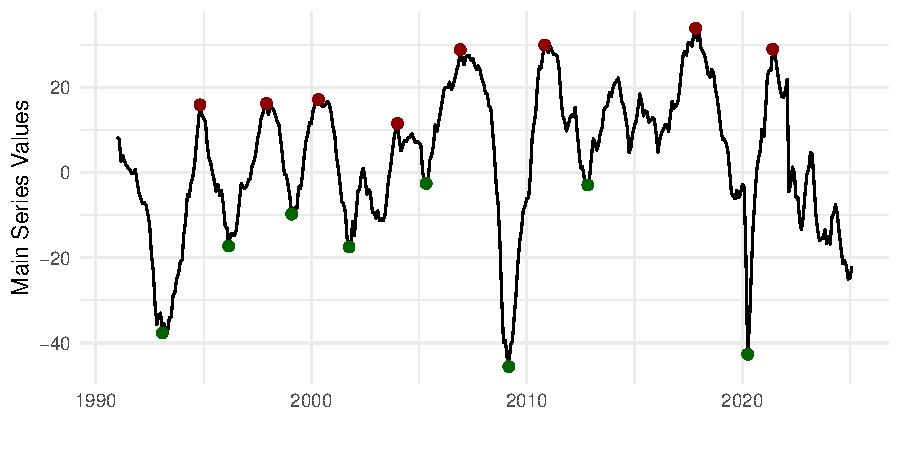
\includegraphics[width=0.5\linewidth]{JakobPlots/BB_main.pdf}
\caption{Bry-Boschan Turning Points of the main index.}
\end{figure}

\subsection{Markov-Regime-Switching}
To simulate a realistic real-time setting for potentially identifying subseries, the Bry-Boschan algorithm is not suitable, as it requires the full data range. Instead, we apply a two-regime Markov-switching model \citep{hamilton1989new}, which allows the system to switch between two regimes, $s_t$, each month and follow the implementation of the R package MSwM \citep{MSwM} for the model. The probability of switching is governed by a latent Markov chain, and each regime is characterized by a different intercept:
\[
y_t = \mu_{s_t} + \epsilon_t , \quad \epsilon_t \sim \mathcal{N}(0,\sigma^2),
\]

Each month, the model provides the probability of switching to the upper regime with a higher intercept in the following month. Following \citet{sauer2023handbook}, we apply a decision rule to classify turning points: if the probability of the upper regime exceeds 0.66 for the first time, it is considered an expansion turning point and if it falls below 0.33 for the first time, it indicates a contraction turning point. Probabilities between 0.33 and 0.66 are treated as uncertain and do not form a strong enough signal for a turning point yet.
\\
The above model can either be run with smoothed probabilities, meaning that the whole data range is used to fit the model, or filtered probabilities, where only data up to the current month $t$ is used. The later one simulates a real-time forecasting scenario and is thus suitable for our evaluation. Note that we did not perform any train-test split to evaluate forecasting models, this is rather a descriptive setting based on the past 30 years. 

\subsection{Classification Task}
Fitting the above to all individual level 1 series gives us turning points for all of these series. To evaluate whether these individual turning points, predicted in real-time, can indicate the groundtruth turning points of the main index, we see it as a classification task. A hit occurs if an actual main turning point follows within a fixed time window after a predicted one. Table~\ref{tab:tp_classification} shows the typical classification metrics we used. However, it also shows how no individual series did bring up any meaningful results, even when tolerating a three months delay for the predicted turning points, compared to the actual ones. 
\begin{table}[H]
\footnotesize
\centering
\begin{subtable}{\linewidth}
    \centering
    \makebox[\textwidth]{%
    \begin{tabular}{lllllllll}
    \toprule
    \textbf{Industry} & \textbf{Question} & \textbf{Hits} & \textbf{Total Pred} & \textbf{Total Actual} & \textbf{Precision} & \textbf{Recall} & \textbf{F1} & \textbf{Lead Time (sd)} \\
    \midrule
    C1900000 & PVS & 7 & 47 & 16 & 0.151 & 0.438 & 0.224 & 2.96 (2.76) \\
    C2000000 & LUS & 4 & 20 & 16 & 0.202 & 0.250 & 0.223 & 5.00 (1.41) \\
    C1300000 & PWS & 4 & 20 & 16 & 0.200 & 0.250 & 0.222 & 4.00 (2.00) \\
    \bottomrule
    \end{tabular}%
    }
    \caption{0 - 6 Months Lead time}
    \label{tab:tp_classification}
\end{subtable}

\vspace{0.5em}
\begin{subtable}{\linewidth}
    \centering
    \makebox[\textwidth]{%
    \begin{tabular}{lllllllll}
    \toprule
    \textbf{Industry} & \textbf{Question} & \textbf{Hits} & \textbf{Total Pred} & \textbf{Total Actual} & \textbf{Precision} & \textbf{Recall} & \textbf{F1} & \textbf{Lead Time (sd)} \\
    \midrule
    C2000000 & QES & 5 & 21 & 16 & 0.312 & 0.312 & 0.312 & -0.60 (2.88) \\
    C1900000 & PVS & 9 & 47 & 16 & 0.196 & 0.562 & 0.291 & 2.17 (3.05) \\
    C1900000 & PWS & 6 & 27 & 16 & 0.225 & 0.375 & 0.280 & 2.00 (3.34) \\
    \bottomrule
    \end{tabular}%
    }
    \caption{-3 - 6 Months Lead time}
\end{subtable}
\end{table}
Since individual series did not appear to provide meaningful signals, we explored grouping multiple series to see if a combined signal could yield a reliable indication. We tested several approaches for aggregating turning points across series: collecting turning points within a rolling window and signaling if a certain threshold was exceeded; averaging their binary states based on the most recent turning point; and averaging the Markov-switching probabilities across series, followed by applying the 0.33/0.66 decision rule. \\
We also used several different approaches to form the groups, such as simply aligning series by their lag value with peak correlation or switching to level 2 and using the groups obtained from CCF-based clustering. However, none of these approaches produced meaningful or interpretable signals.
\subsubsection{Grouped Series - Flipped}
However, a small effect was observed when noting that, for some groups, the approximate number of turning points roughly matched the number of ground-truth turning points. For instance, considering all series with peak CCFs at lags -1, 0, and 1, so series with roughly synchronous characteristics. Their turning points were lagging quite far behind the Bry-Boschan turning points of the main index, potentially also simply due to the nature of using a Markov switching model with differing intercepts. But flipping the prediction goal and predicting opposite turning points, predicting contraction points as expansions and vice versa, the subseries do seem to roughly indicate main turning points. Whether this has any actual value is open, but a potential interpretation might be that once even these groups have reached the current regime according to their Markov switching probability, it might soon be over and a turning point could occur in the next twelve months. Fig.~\ref{fig:flipped_turningpoints} shows the turning points of the above group compared to the main ones and table~\ref{tab:flipped_turningpoints} the scores when evaluating according to this flipped scenario. 

\begin{figure}[H]
    \centering
    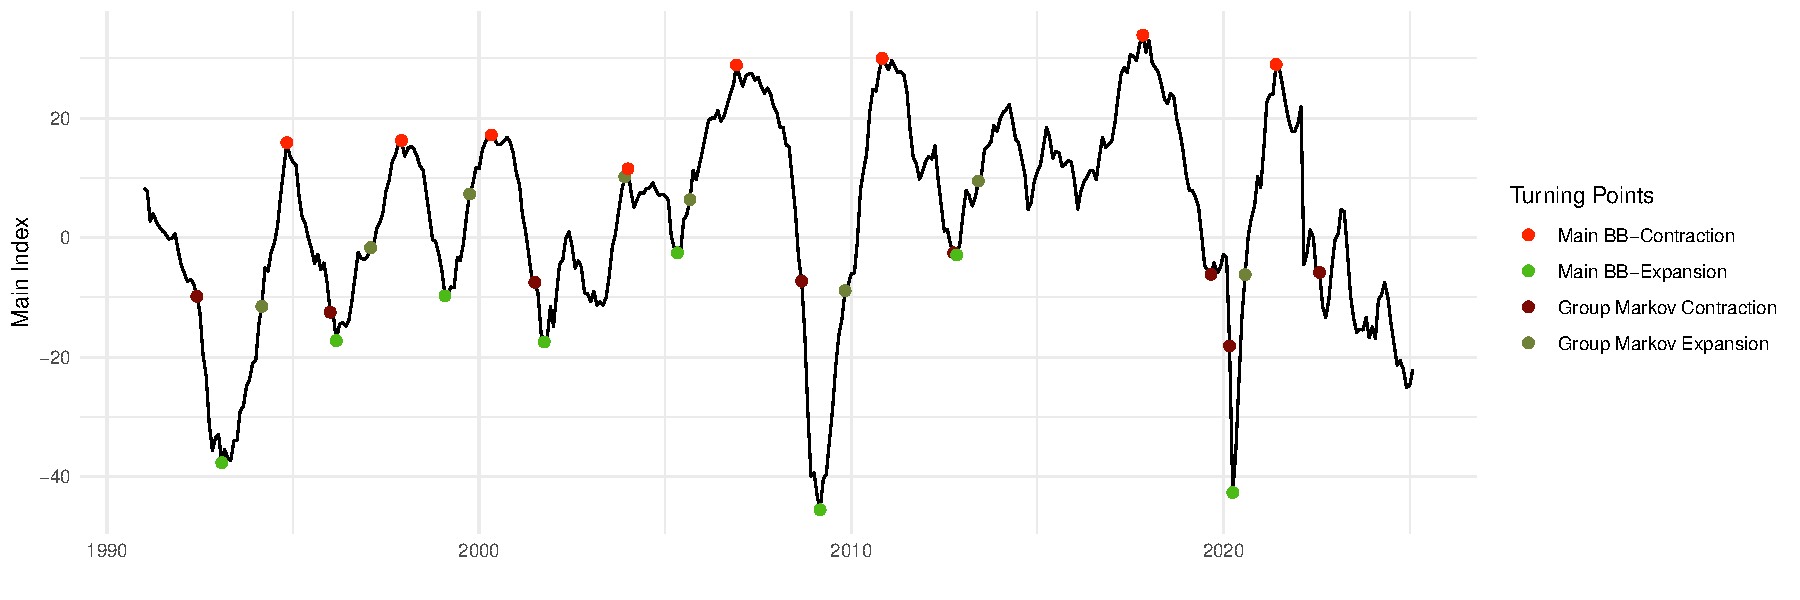
\includegraphics[width=\linewidth]{JakobPlots/Lag1_3_cluster_turningpoints_main.pdf}
    \caption{Turning points of group of all level 1 series with roughly composite moving characteristics according to their peak CCF lag value.}
    \label{fig:flipped_turningpoints}
\end{figure}

\begin{table}[H]
\centering
\footnotesize
\makebox[\textwidth]{%
\begin{tabular}{lllllllll}
\toprule
\textbf{Main Type} & \textbf{Hits} & \textbf{Total Pred} & \textbf{Total Actual} & \textbf{Precision} & \textbf{Recall} & \textbf{F1} & \textbf{Lead Time (sd)}\\
\midrule
Expansion & 6 & 7 & 8 & 0.857 & 0.75 & 0.8 & 5.67 (3.78) \\
Contraction & 6 & 8 & 8 & 0.75 & 0.75 & 0.75 & 3.17 (3.37) \\
\bottomrule
\end{tabular}
}
\caption{Evaluation of the flipped indication setting.}
\label{tab:flipped_turningpoints}
\end{table}

\newpage
%--------------------------------------------------------------------------------

%--------------------------------------------------------------------------------
\section{Conclusion}
\label{ch:conclusion}
This consulting project examined the internal structures of the ifo Business Survey (1991–2025) with the aim of detecting systematic relationships between the main index and the underlying time series. Rather than building a full forecasting model, the focus was on identifying small \emph{predictive subsets} of industries which stick out as especially important for the overall index. We find strong correlations with clear lead–lag structures within $\pm6$ months that compress during crises, pointing to their role as early stress signals. While most industries are Granger causal, their individual contribution is negligible, which emphasizes the importance of subsets and clusters. The time series showing up across the various grouping and clustering approaches of our analysis often contained industries which are rather early in the supply chain or investment related. 

\paragraph{Correlation Analysis}
The analysis reveals strong dependencies between industry indicators and the main manufacturing index, concentrated within a $\pm6$ month window. Despite sectoral imbalance and non-stationarity, the correlation structure remains coherent and economically meaningful. Consensus results further show that correlations compress during crises, suggesting that shifts in industry alignment may provide early signals of systemic stress and warrant deeper investigation.

\paragraph{Granger Causality}
Almost all manufacturing industries are Granger causal (simple and instantaneous) to the aggregate main-index. The contribution of any single industry is minimal in terms of information gain measured by adjusted $R^2$. Additionally an implicit requirement for Granger causality is stationarity which is violated in some survey questions and industries (see \ref{stationarity}). Thus, we find this method to be rather unsuitable for further analysis and insights. 

\paragraph{Elastic Net vs.\ Scoring Model.}
Both methods improve on the benchmark of lagged main-index values. Compared to 500 random five-industry subsets, they perform better in the early prediction set, likely because overfitting is harder there, while the general prediction set leaves more scope for spurious fit. Although the exact industry codes differ, both approaches consistently select sectors linked to inputs, packaging, and investment goods. From an economic perspective, these sectors are upstream in the value chain and therefore tend to adjust production earlier, making them natural candidates for anticipating aggregate manufacturing dynamics.

\paragraph{CCF clustering.}
We also clustered individual survey questions (level 2) by their cross-correlation with the main index. To compare the clusters, we fitted linear models with lagged values of cluster average cluster and lagged values of the main index itself to the main index. We combined it with visually assessing the cross-correlation function to identify potentially leading and interesting clusters. 
Especially the early prediction setting brought out some leading clusters. While many clusters are hard to interpret, clearer examples feature intermediate goods and investment-related activities. 

\paragraph{Turning points.}
Trying to explicitly indicate turning points and not just the main index itself was evaluated separately. We used the Bry-Boschan algorithm to identify turning points of the main index and Markov Switching models for potentially indicating turning points of the subseries. Neither individual nor grouped series were able to reliably indicate the Bry-Boschan turning points of the main index, when modeling their levels with Markov Switching. Further smoothing the series and applying Markov switching models to model the first differences or other more sophisticated approaches could be examined in further analysis. 

\paragraph{Outlook.}
Taken together, the results show that the underlying time series of the ifo Business climate are able to provide meaningful information beyond the main index alone. Future work could explore the data in greater depth, as many of our results suggested points to further elaborate on. Also, our analysis was restricted to the monthly questions of the manufacturing industry. Taking all of the 40.000 time series of the survey into account, could lead to many more insights. 



\newpage
%--------------------------------------------------------------------------------
%--------------------------------------------------------------------------------
\section{Contributions}
\label{ch:contributions}

Jakob Freytag wrote the Introduction, the Turning Point Indication chapters, the CCF based clustering and the respective code. He also coded the data pre-processing.
Dominik Pitz wrote the chapters on Correlation Analysis and Indicative Subsets with the respective Code.
Daniel Gloukhman wrote the chapter on Granger Causality and the respective code. He also wrote the code to import and combine the ifo-dataset.\\
%Coding and especially commenting the code was aided by ChatGPT and Gemini.
We used generative AI-tools like ChatGPT and Gemini for refining grammar, text style and improving readability of this report. Further, these tools also aided us in coding and especially in commenting the code. 
\newpage
%--------------------------------------------------------------------------------

%--------------------------------------------------------------------------------
\section{Appendix}
\label{ch:appendix}
\input{chapters/appendix}
\newpage
%--------------------------------------------------------------------------------


%--------------------------------------------------------------------------------
\pagenumbering{Roman}
\setcounter{page}{4} % CHANGE


\clearpage

\bibliographystyle{dcu}
\bibliography{bibliography}

\clearpage

\section{Electronic Supplement}
The source-code for this report and the statistical analysis can be found on Github at \href{https://github.com/dgloukhman/ifo-lmu-consulting}{https://github.com/dgloukhman/ifo-lmu-consulting}. The survey data is not public and can be obtained from the ifo Institute. 


\end{document}